\subsection{Дифференциальные уравнения}
	
	\subsubsection{Аннотация}

		Курс <<Дифференциальные уравнения>>, в целом, получил положительные отзывы. Острых проблем с курсом не было выявлено.

	\subsubsection{Общий отзыв студентов о курсе}

		\begin{figure}[H]
			\centering
			\begin{subfigure}[b]{0.45\textwidth}
				\centering
				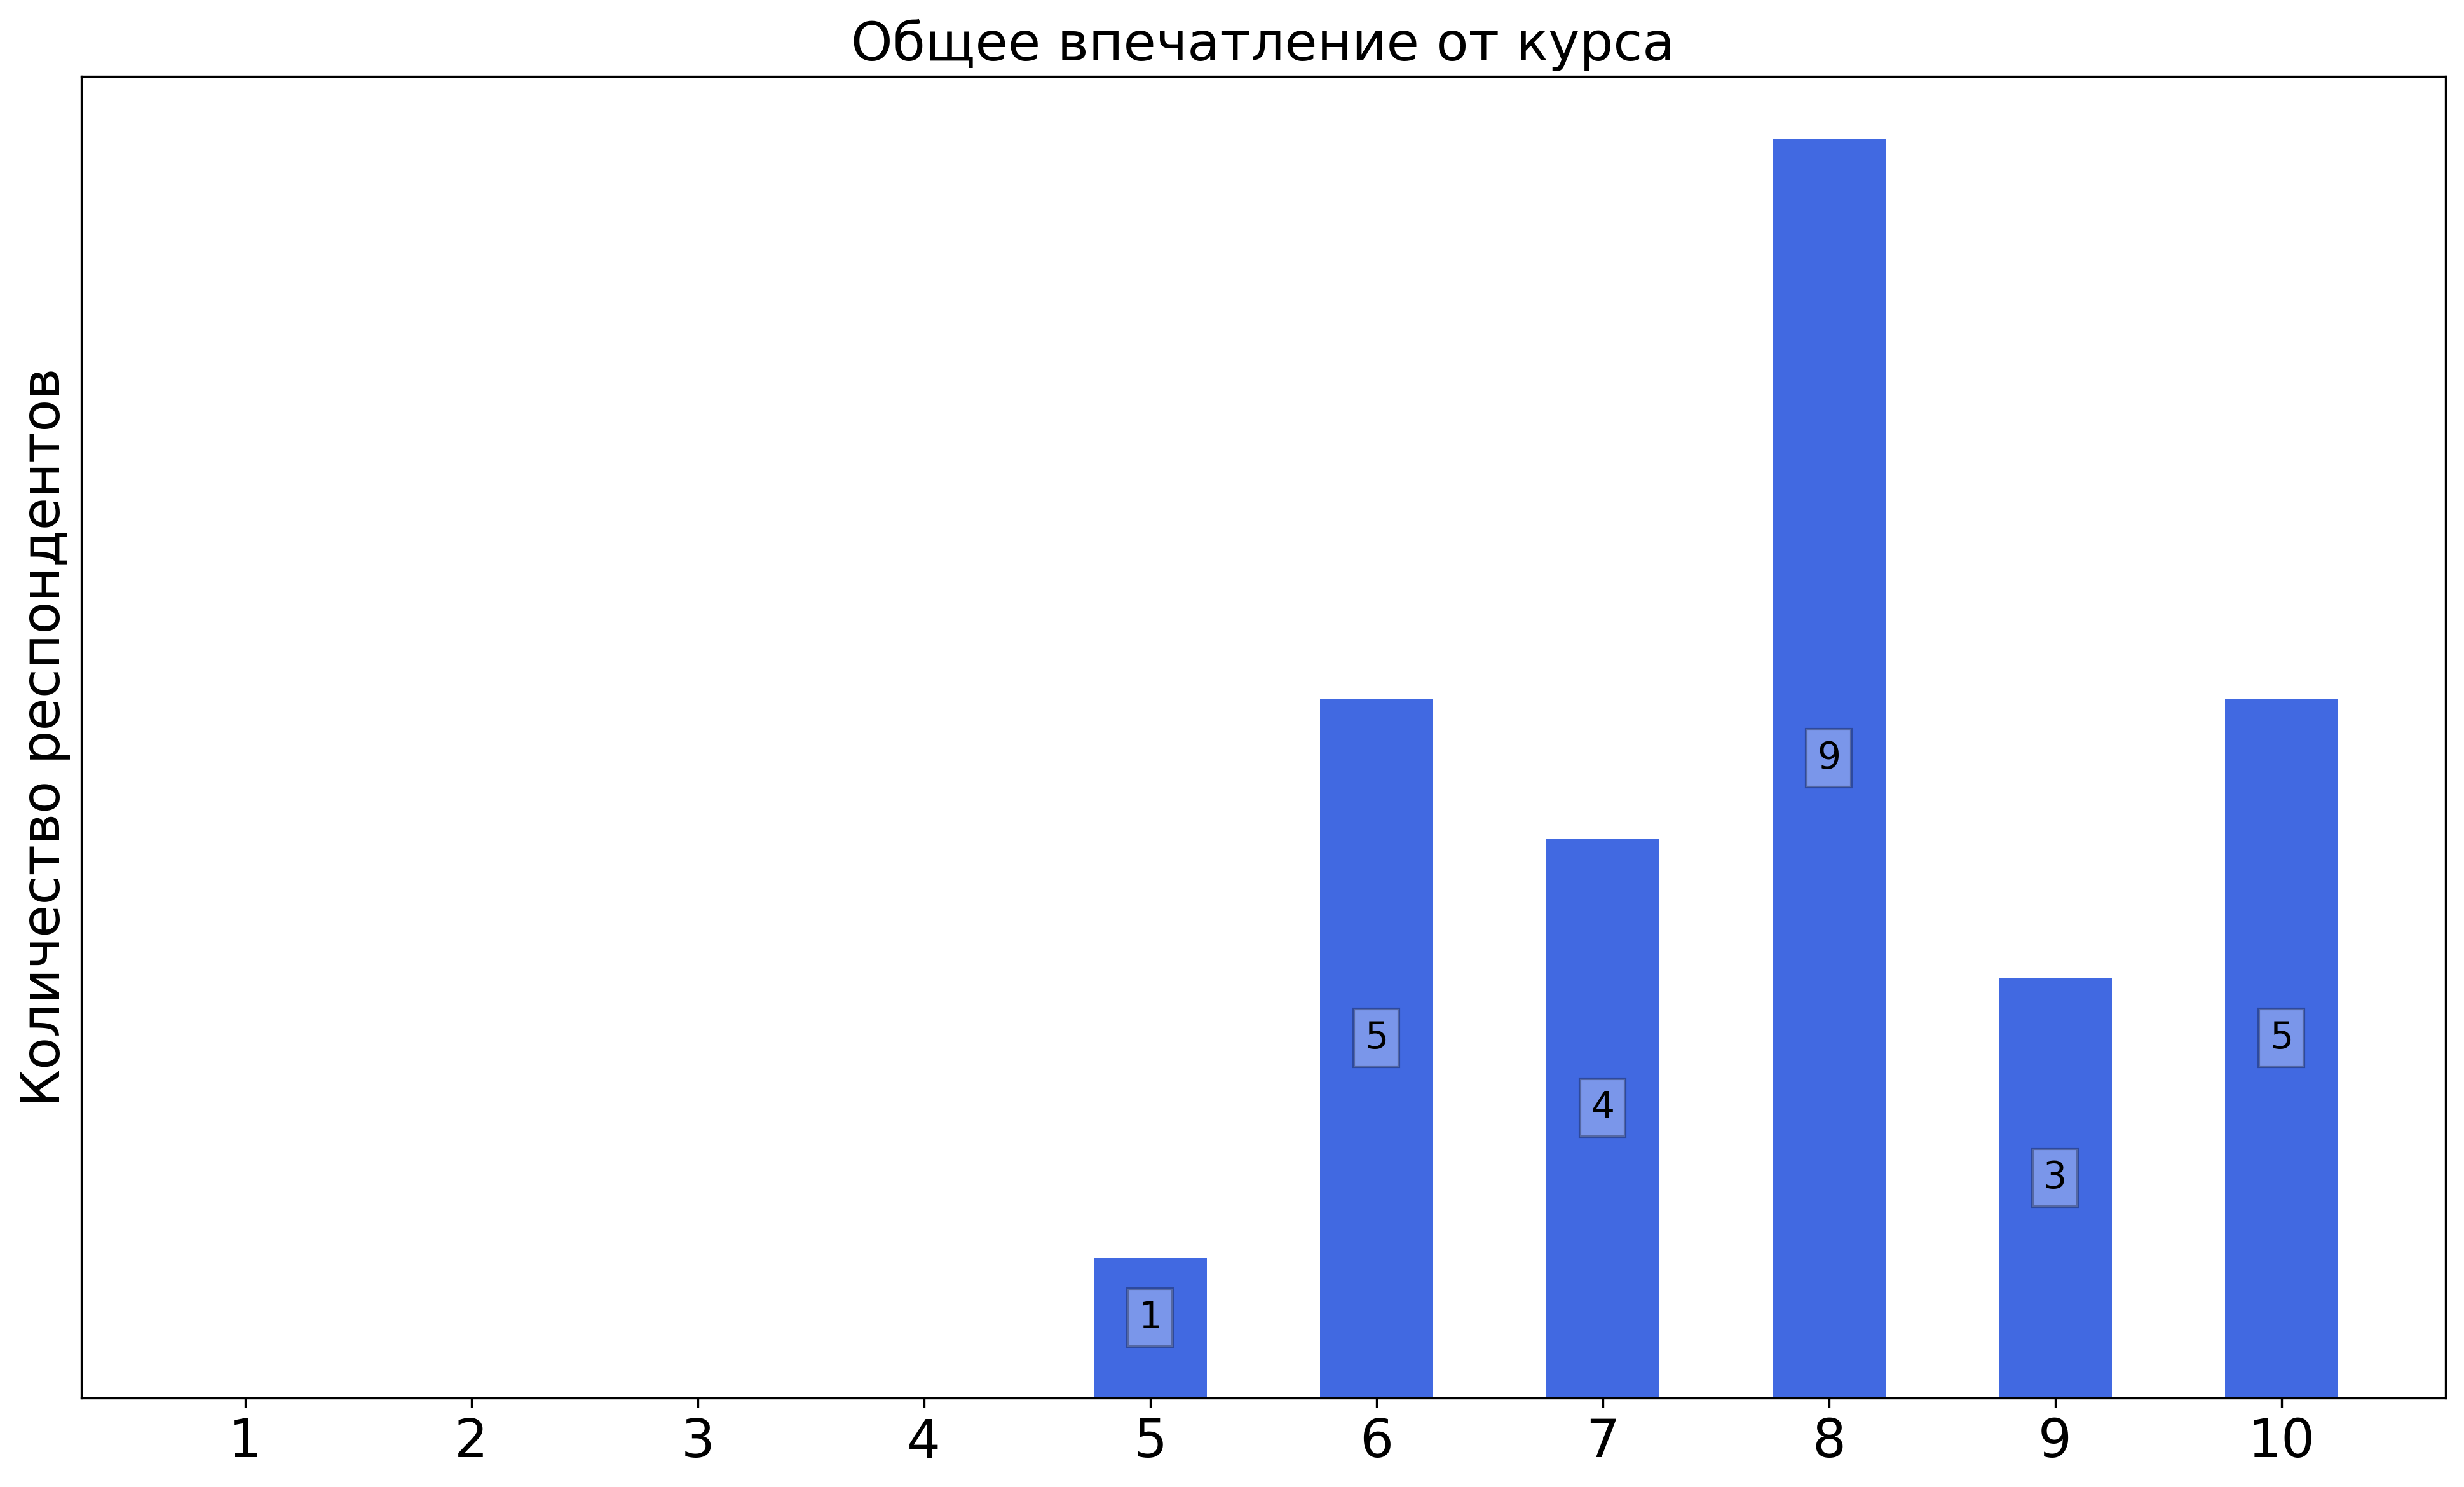
\includegraphics[width=\textwidth]{images/2 course/Дифференциальные уравнения/general-0.png}
			\end{subfigure}
		\end{figure}

	\subsubsection{Материалы, использумые респондентами при изучении курса}

		\begin{figure}[H]
			\centering
			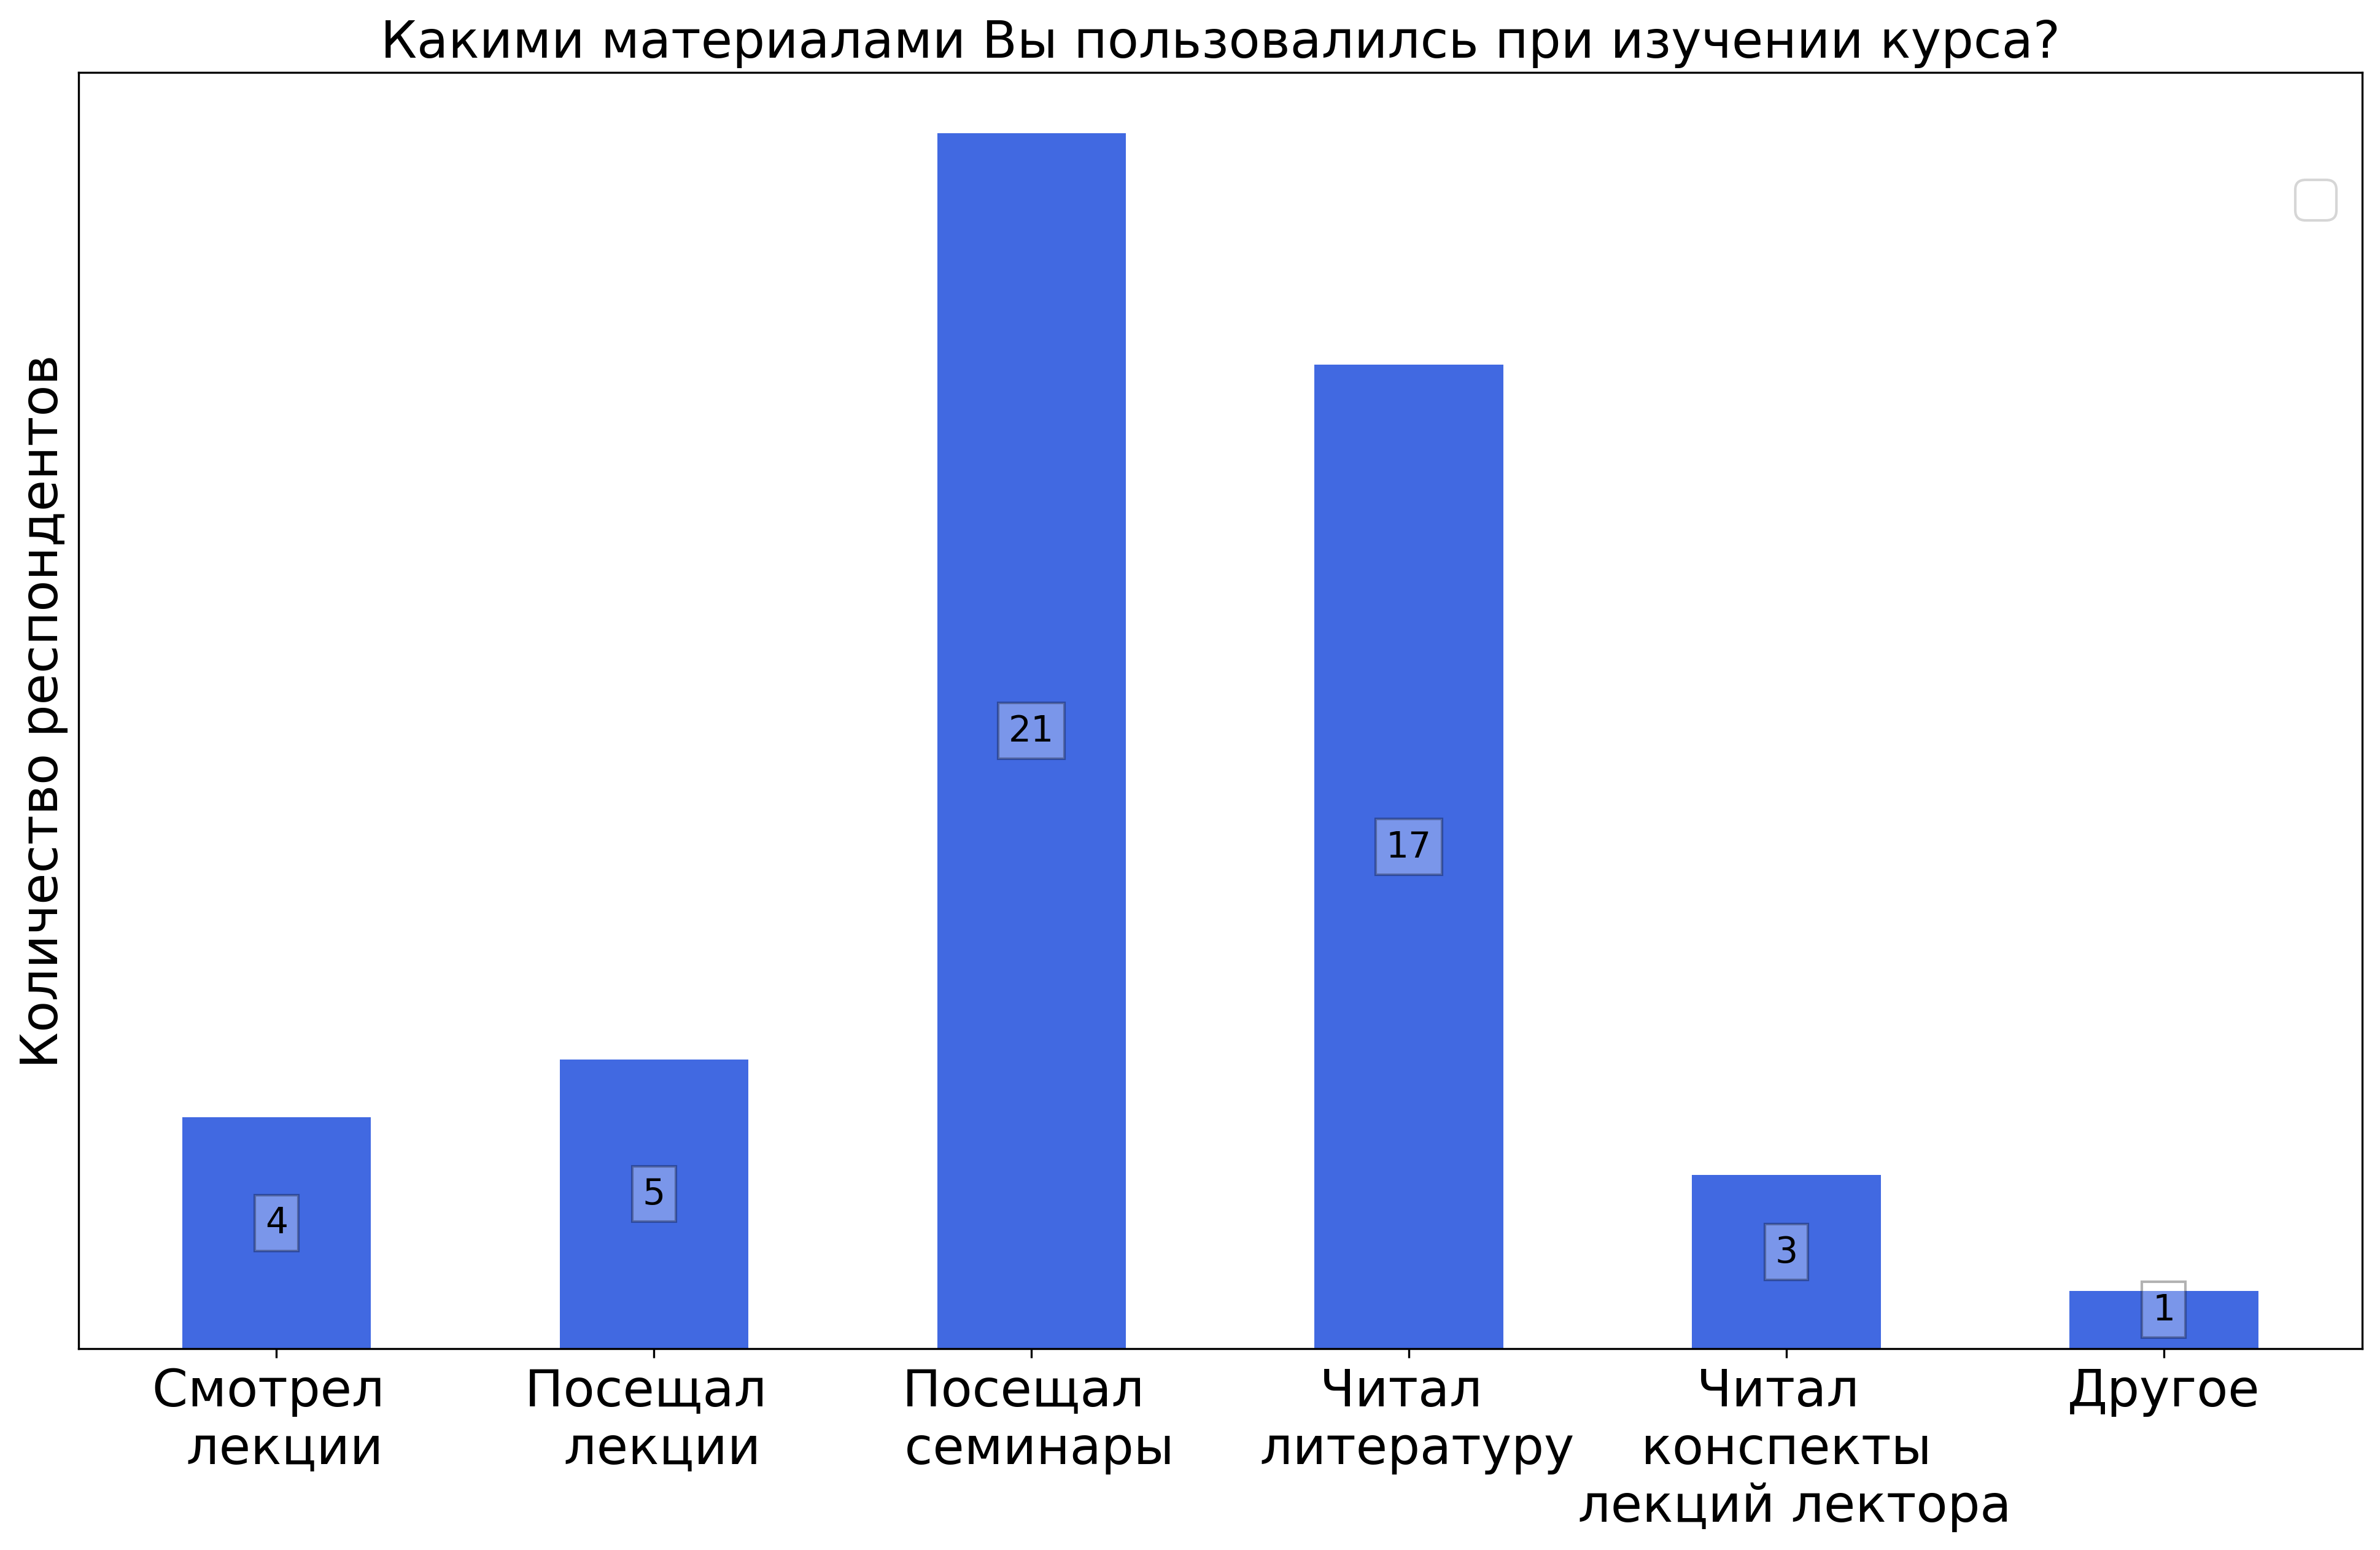
\includegraphics[width = 0.45\textwidth]{images/2 course/Дифференциальные уравнения/materials.png}
		\end{figure}

		\textit{В качестве других источников информации студенты указали:} 
		\begin{itemize}
            \item записи семинаров других преподавателей.
		\end{itemize}

	\subsubsection{Отзыв студентов о лекциях. Лектор: Бишаев А.М.}

		\begin{figure}[H]
			\centering
            \begin{subfigure}[b]{0.45\textwidth}
				\centering
				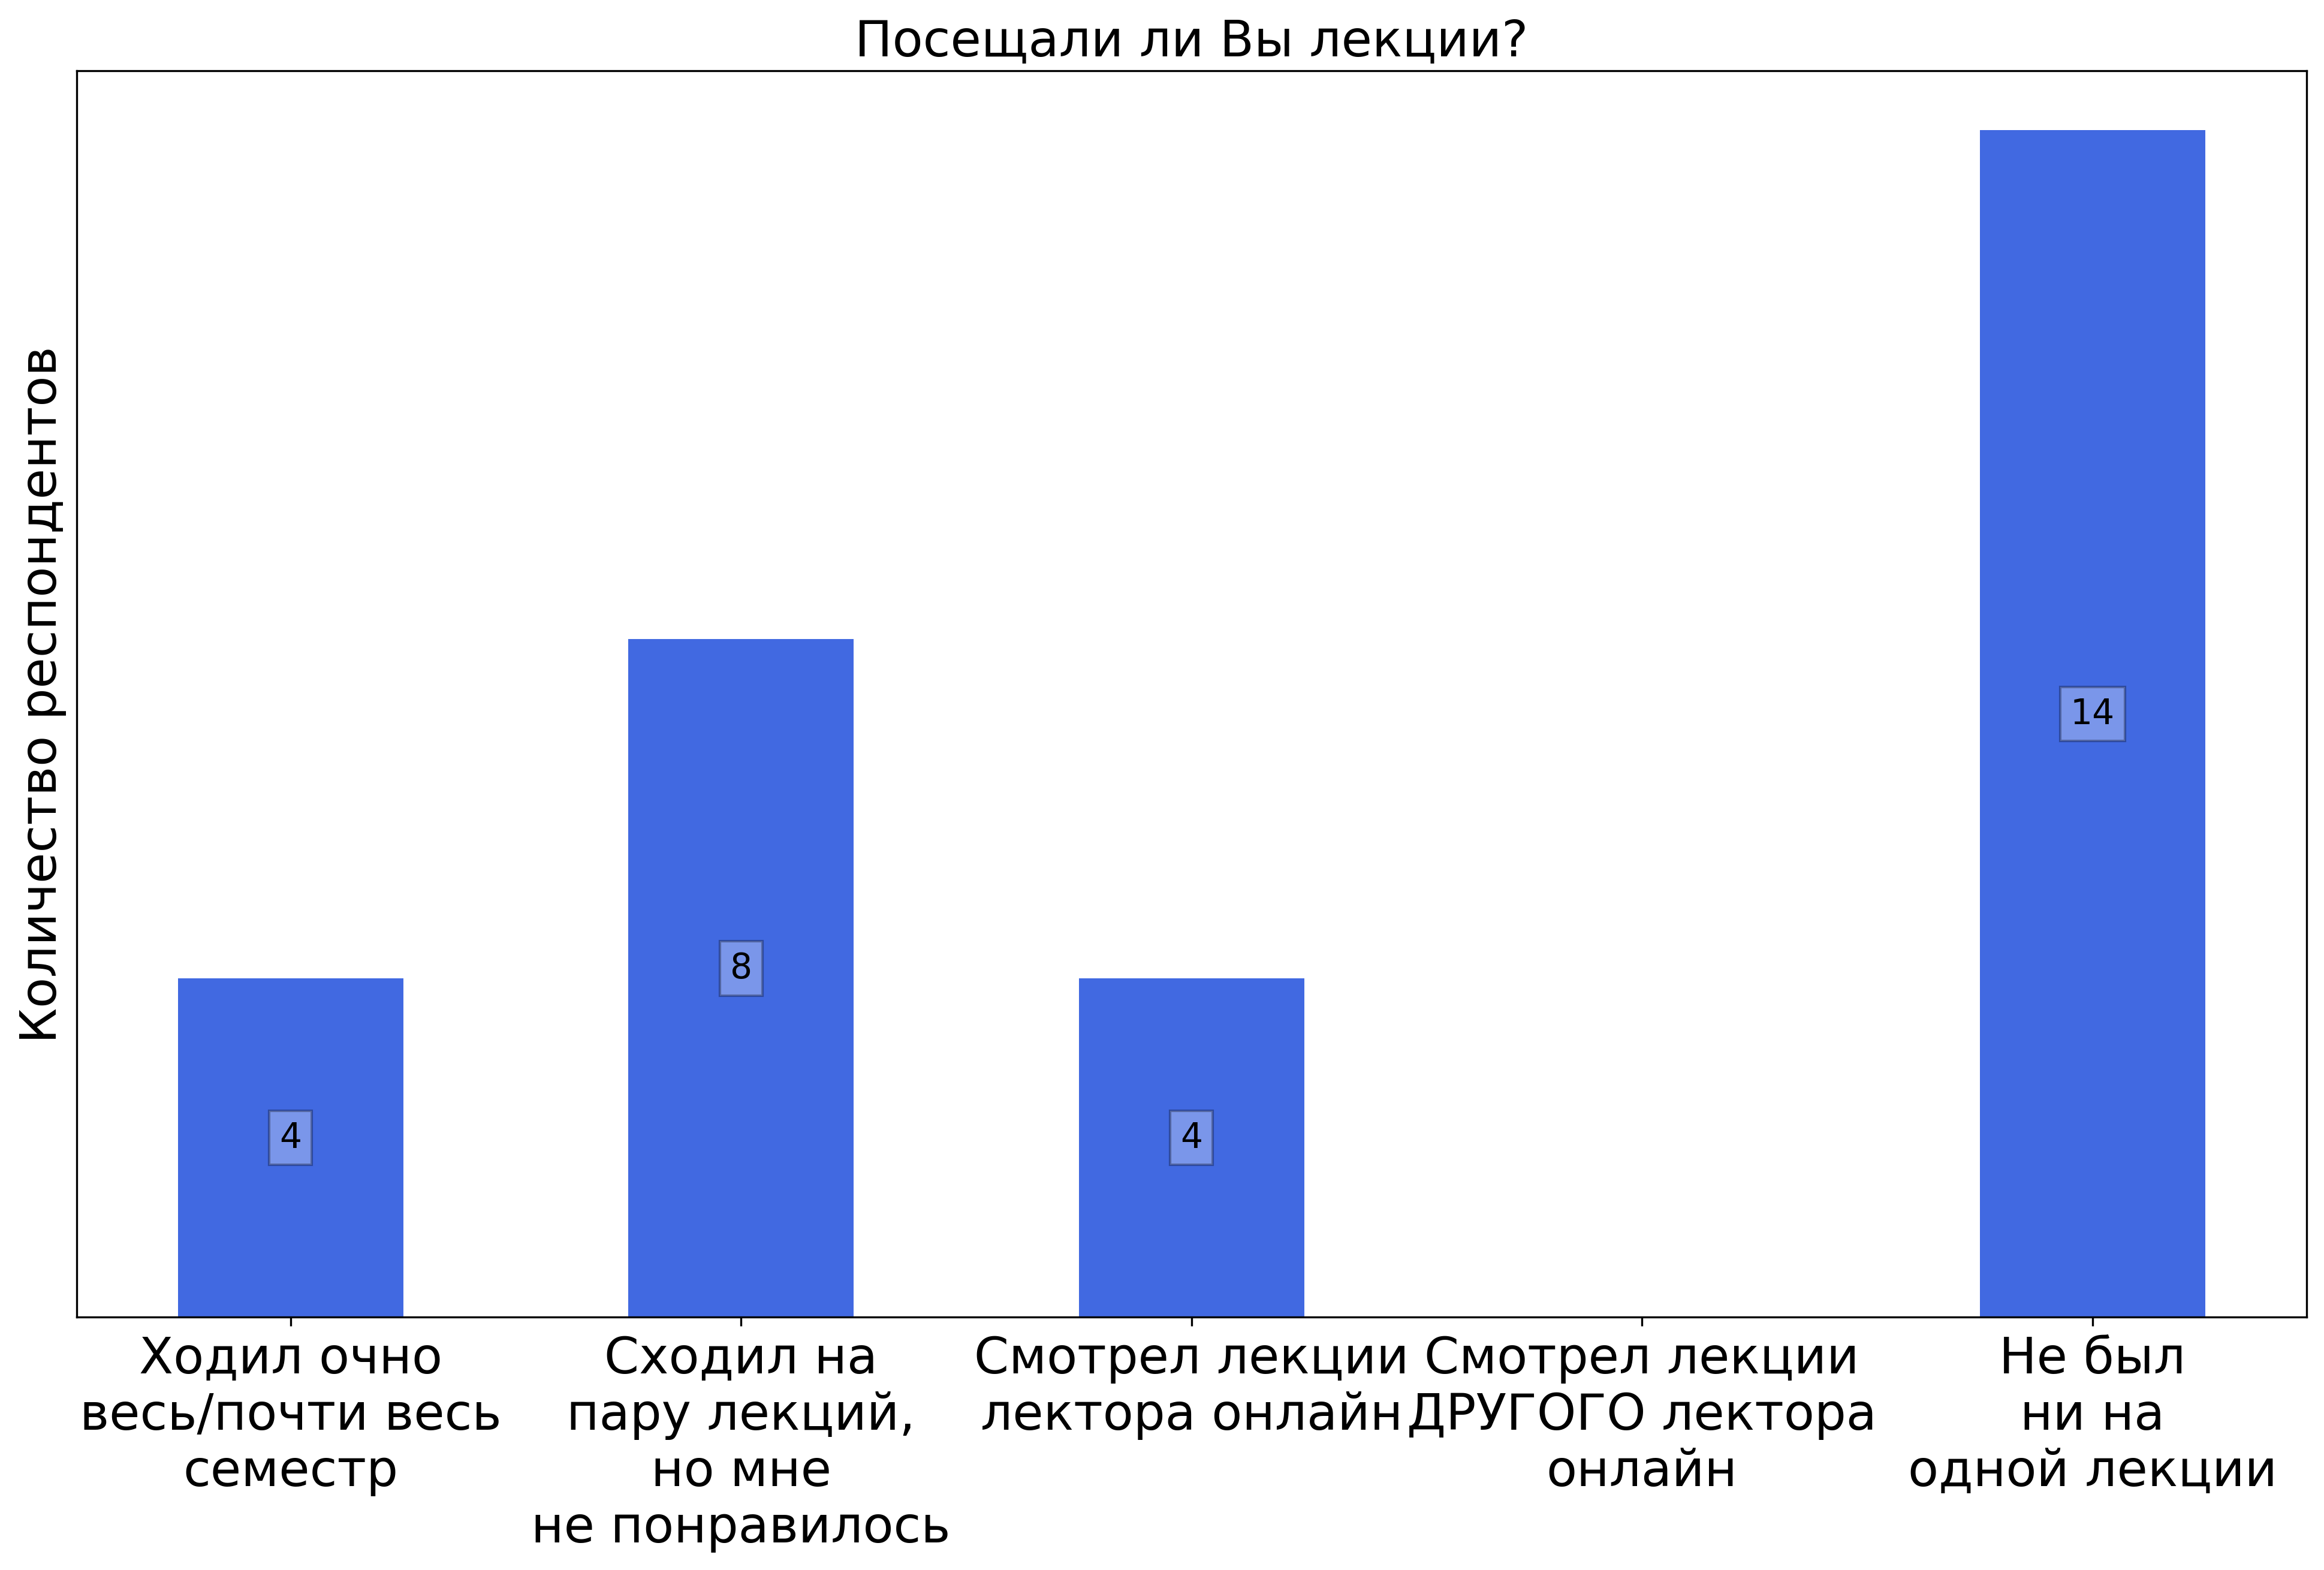
\includegraphics[width=\textwidth]{images/2 course/Дифференциальные уравнения/lecturer-questions-Бишаев А.М.-0.png}
			\end{subfigure}
			\begin{subfigure}[b]{0.45\textwidth}
				\centering
				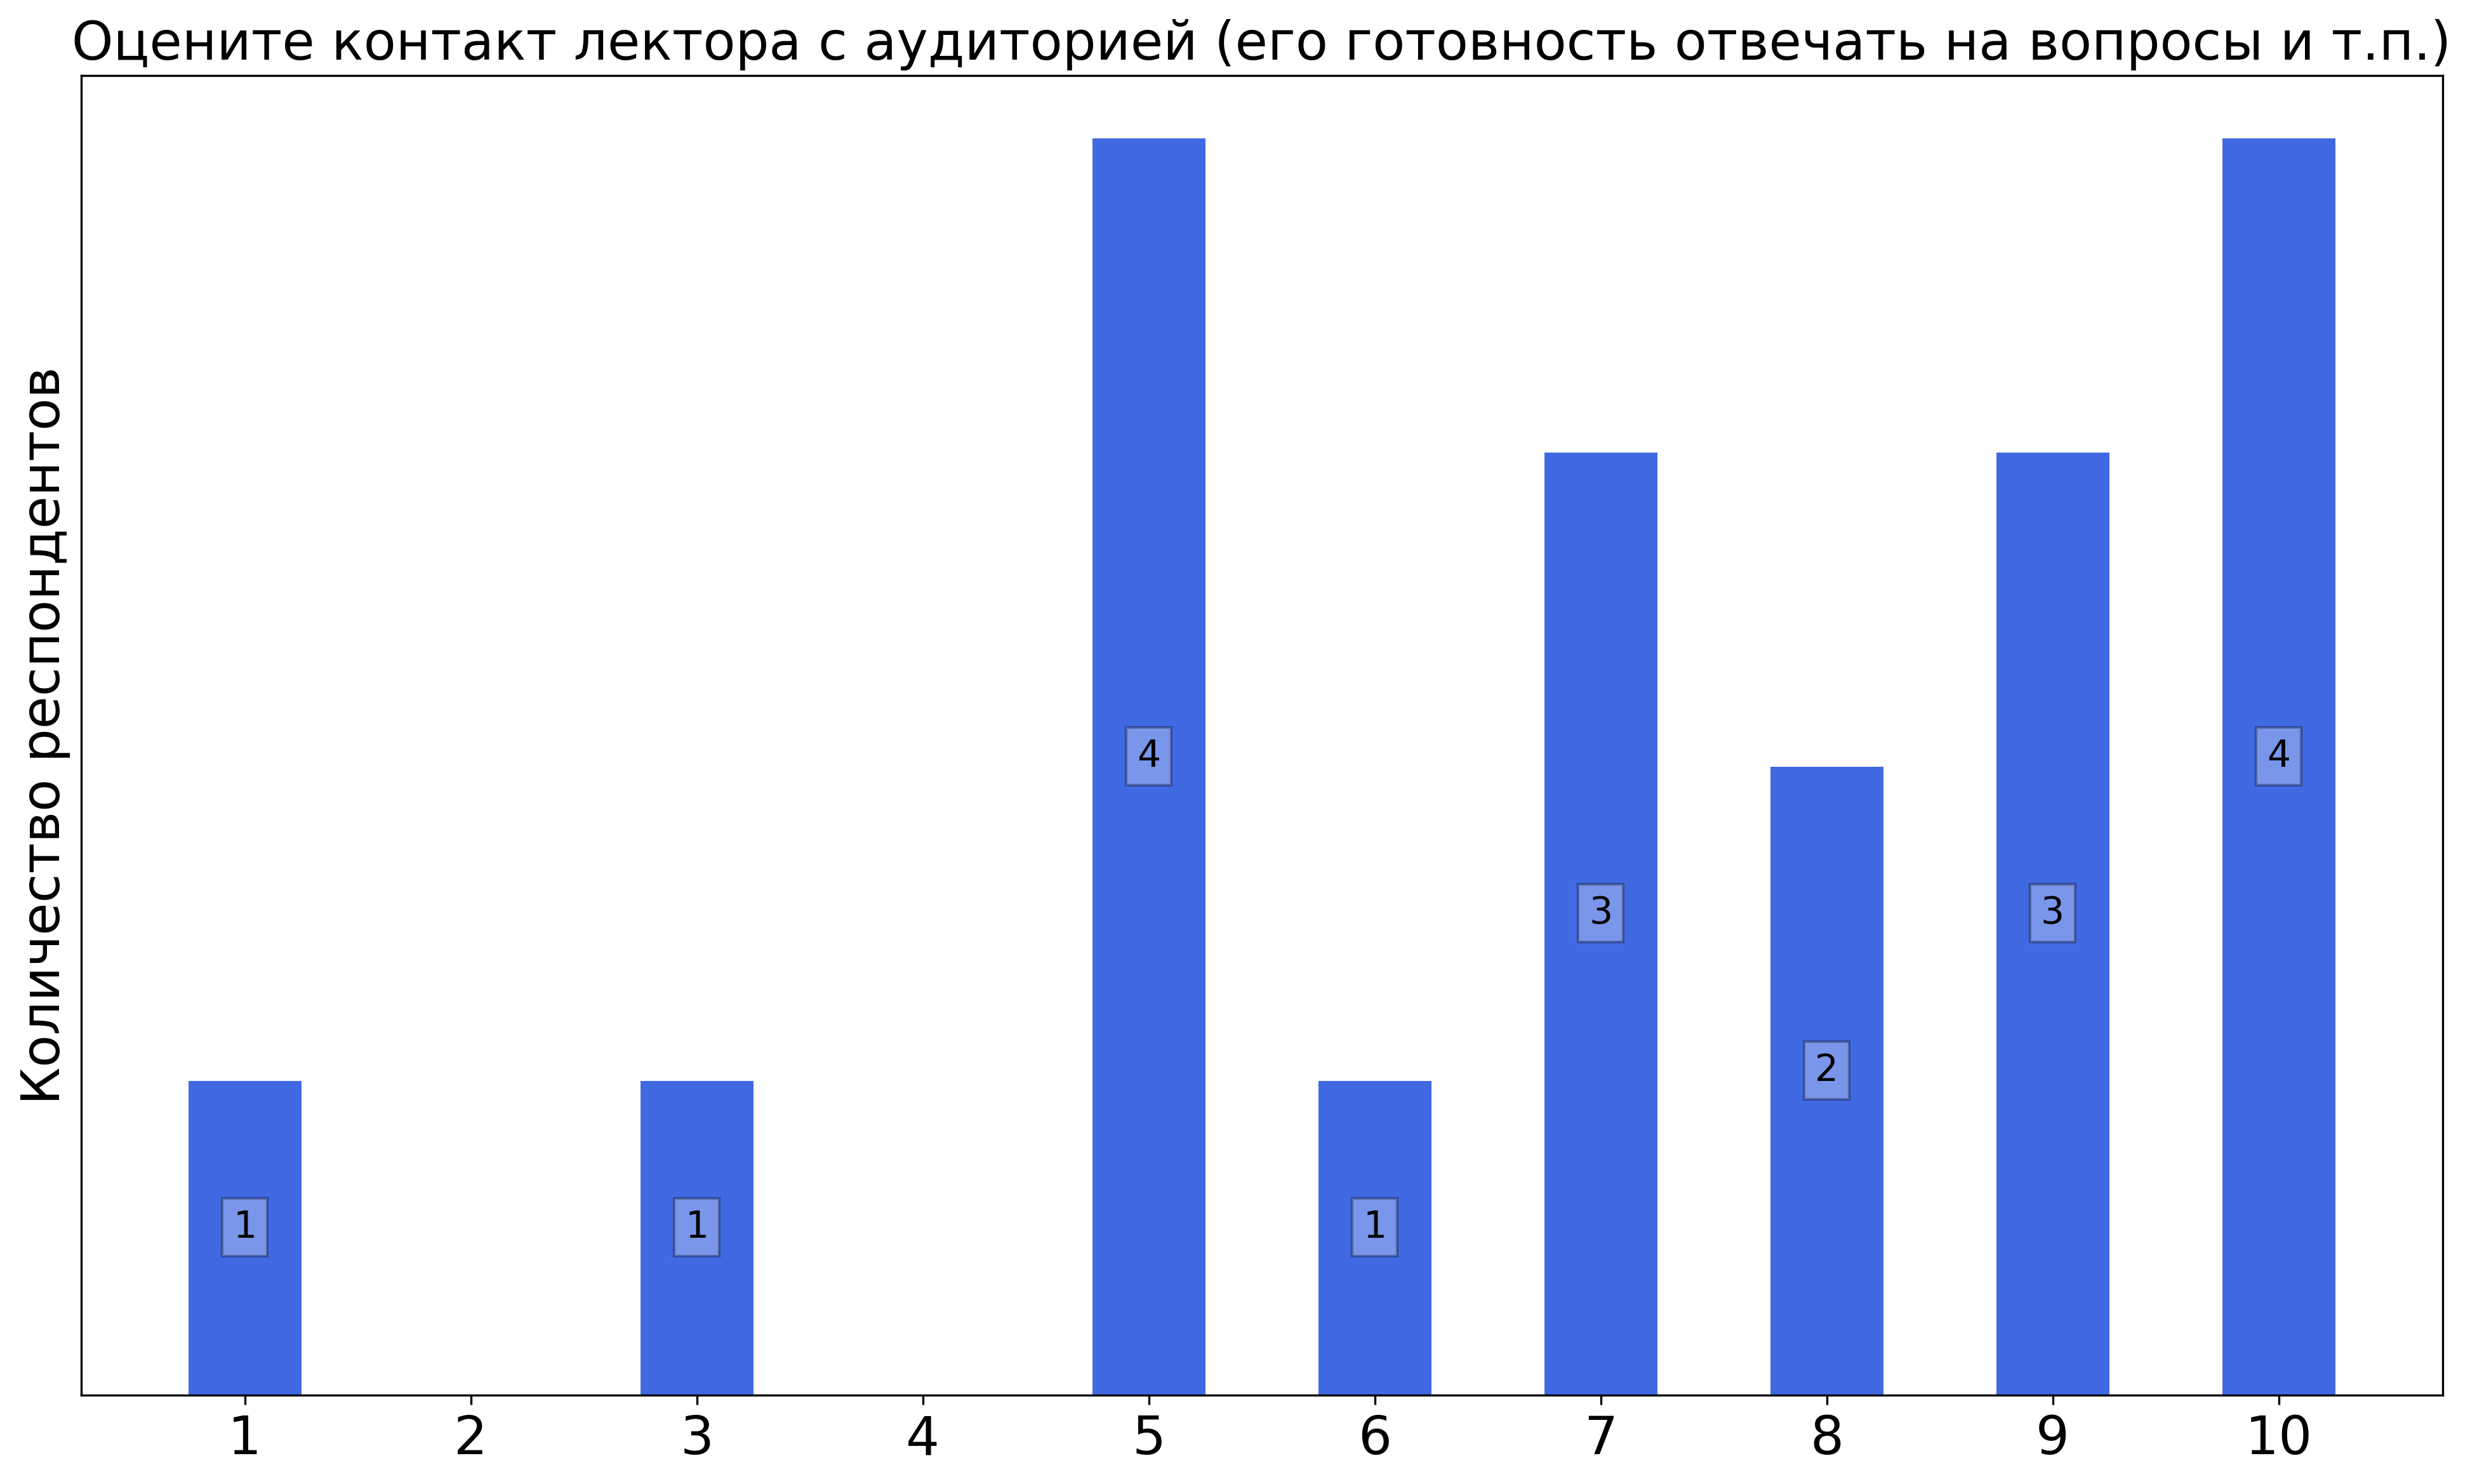
\includegraphics[width=\textwidth]{images/2 course/Дифференциальные уравнения/lecturer-marks-Бишаев А.М.-0.png}
			\end{subfigure}
			\begin{subfigure}[b]{0.45\textwidth}
				\centering
				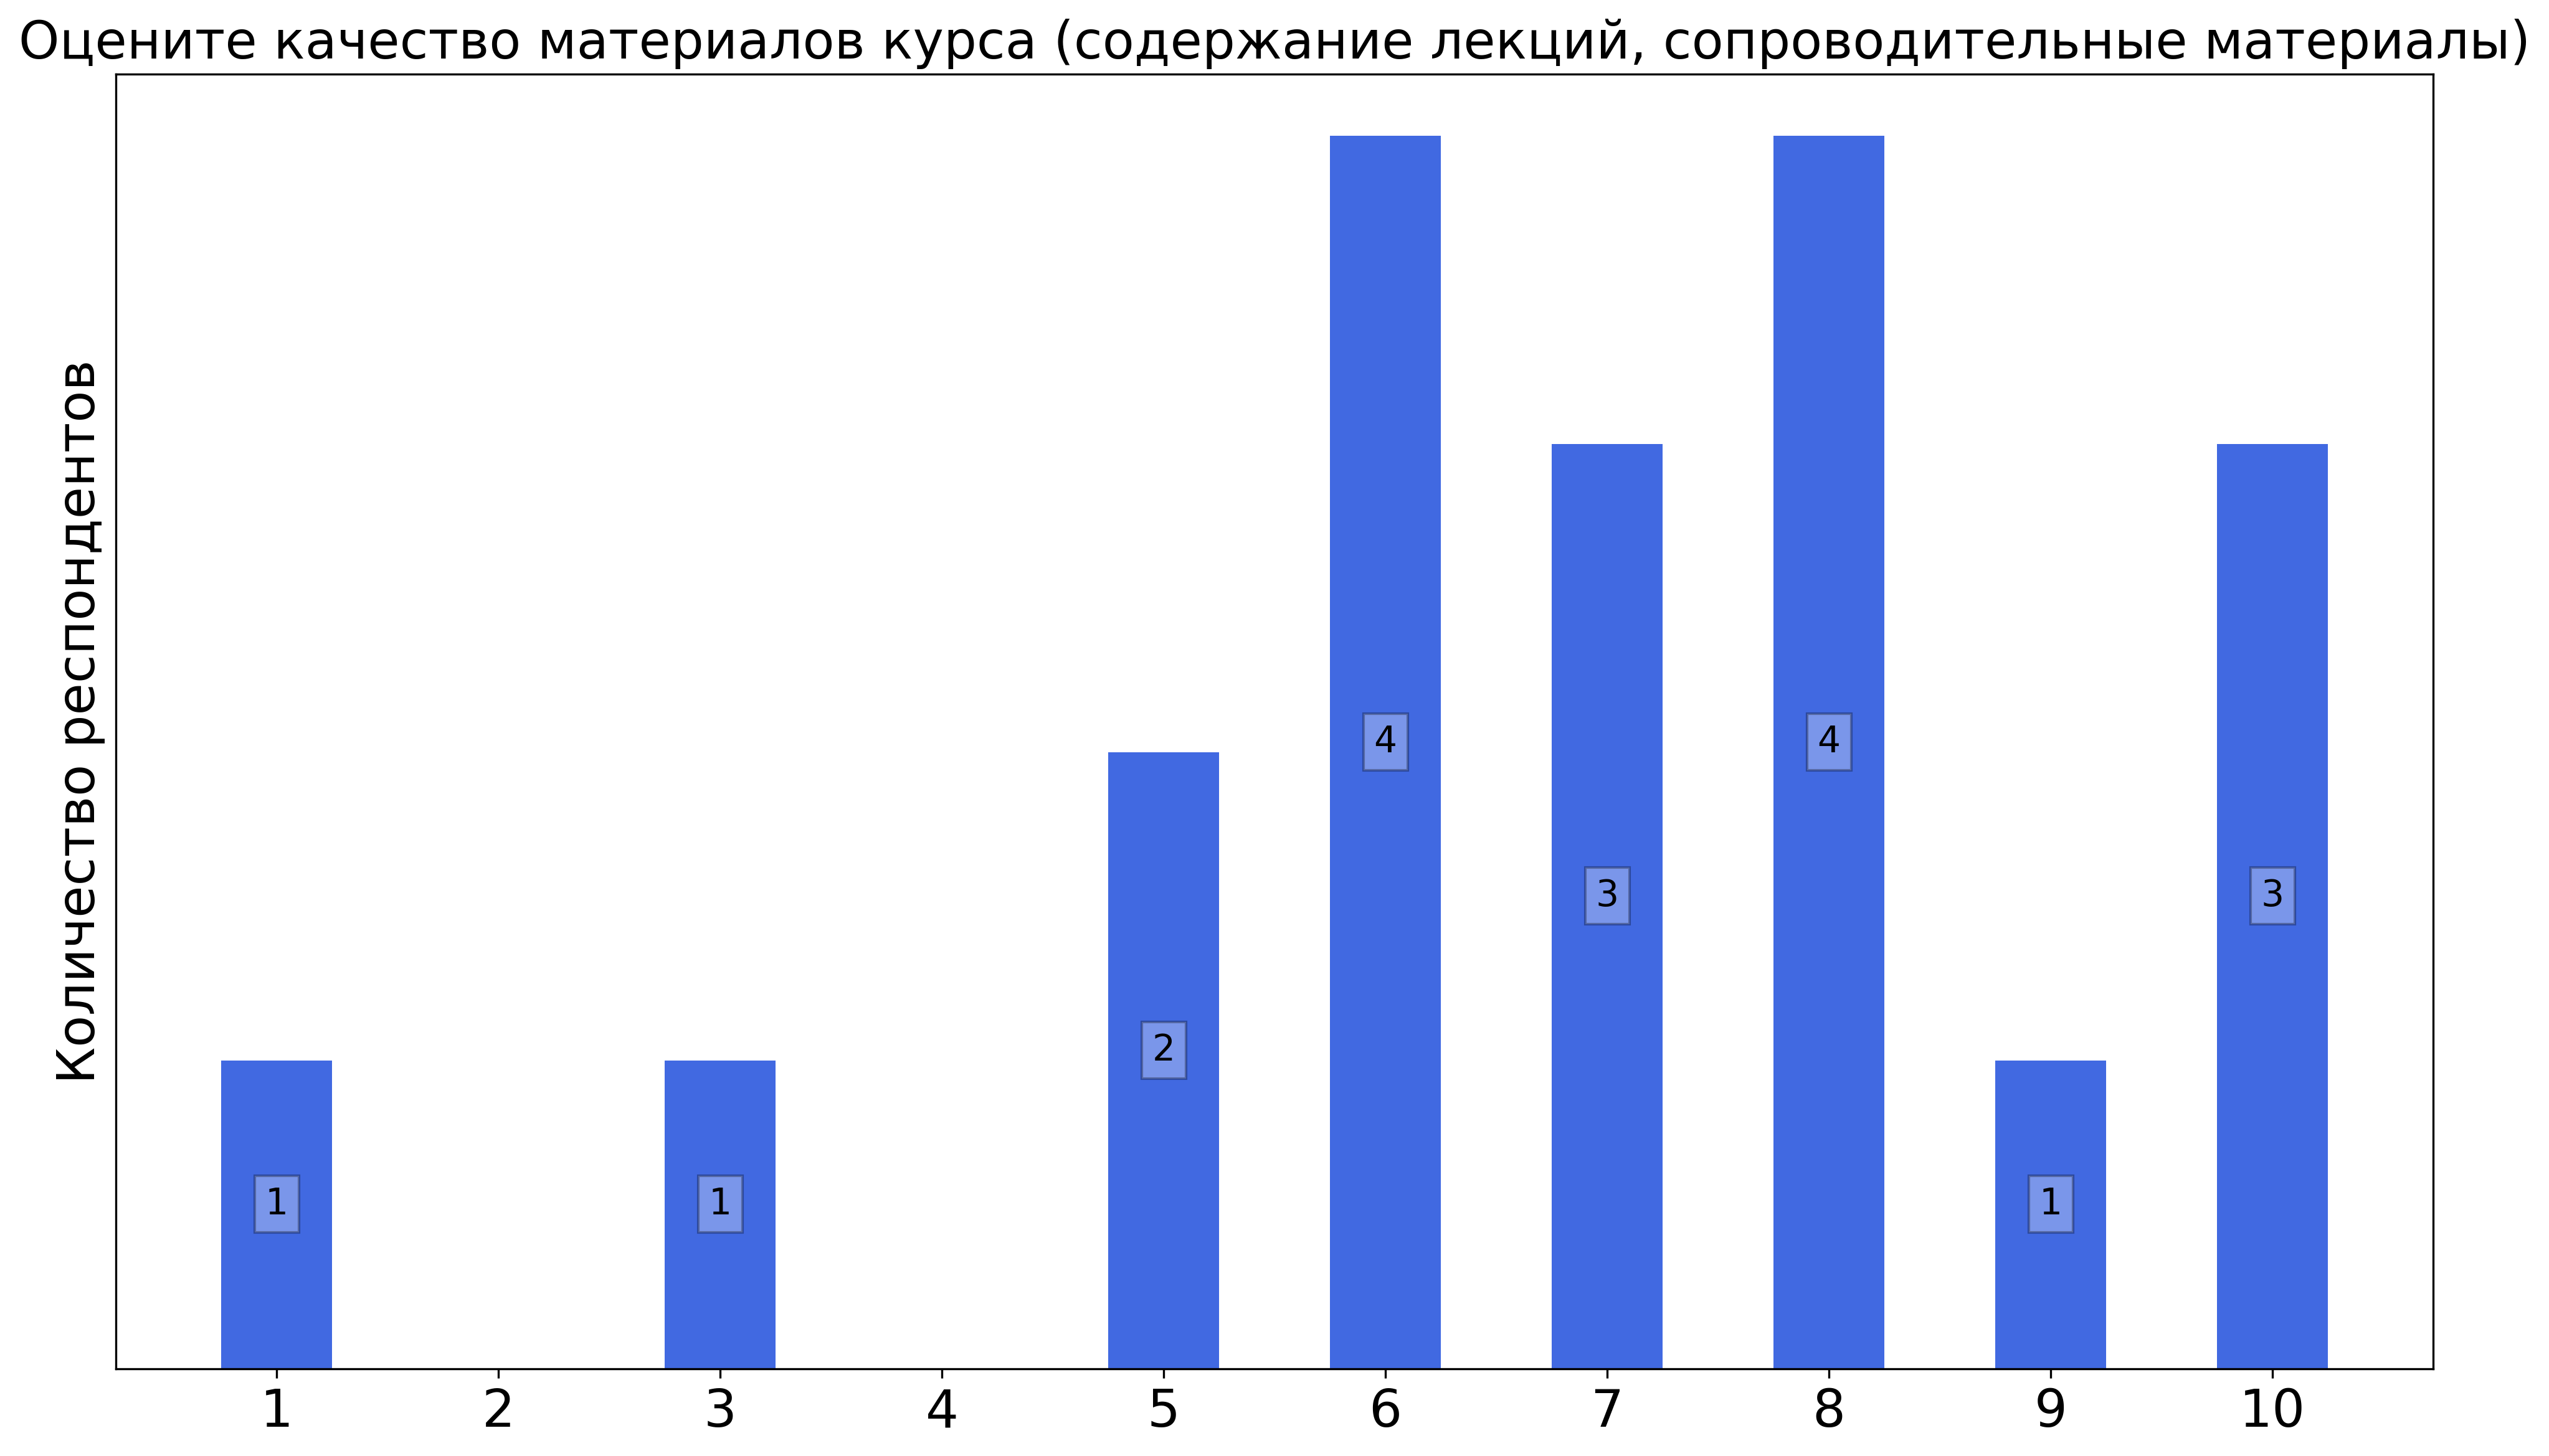
\includegraphics[width=\textwidth]{images/2 course/Дифференциальные уравнения/lecturer-marks-Бишаев А.М.-1.png}
			\end{subfigure}
			\begin{subfigure}[b]{0.45\textwidth}
				\centering
				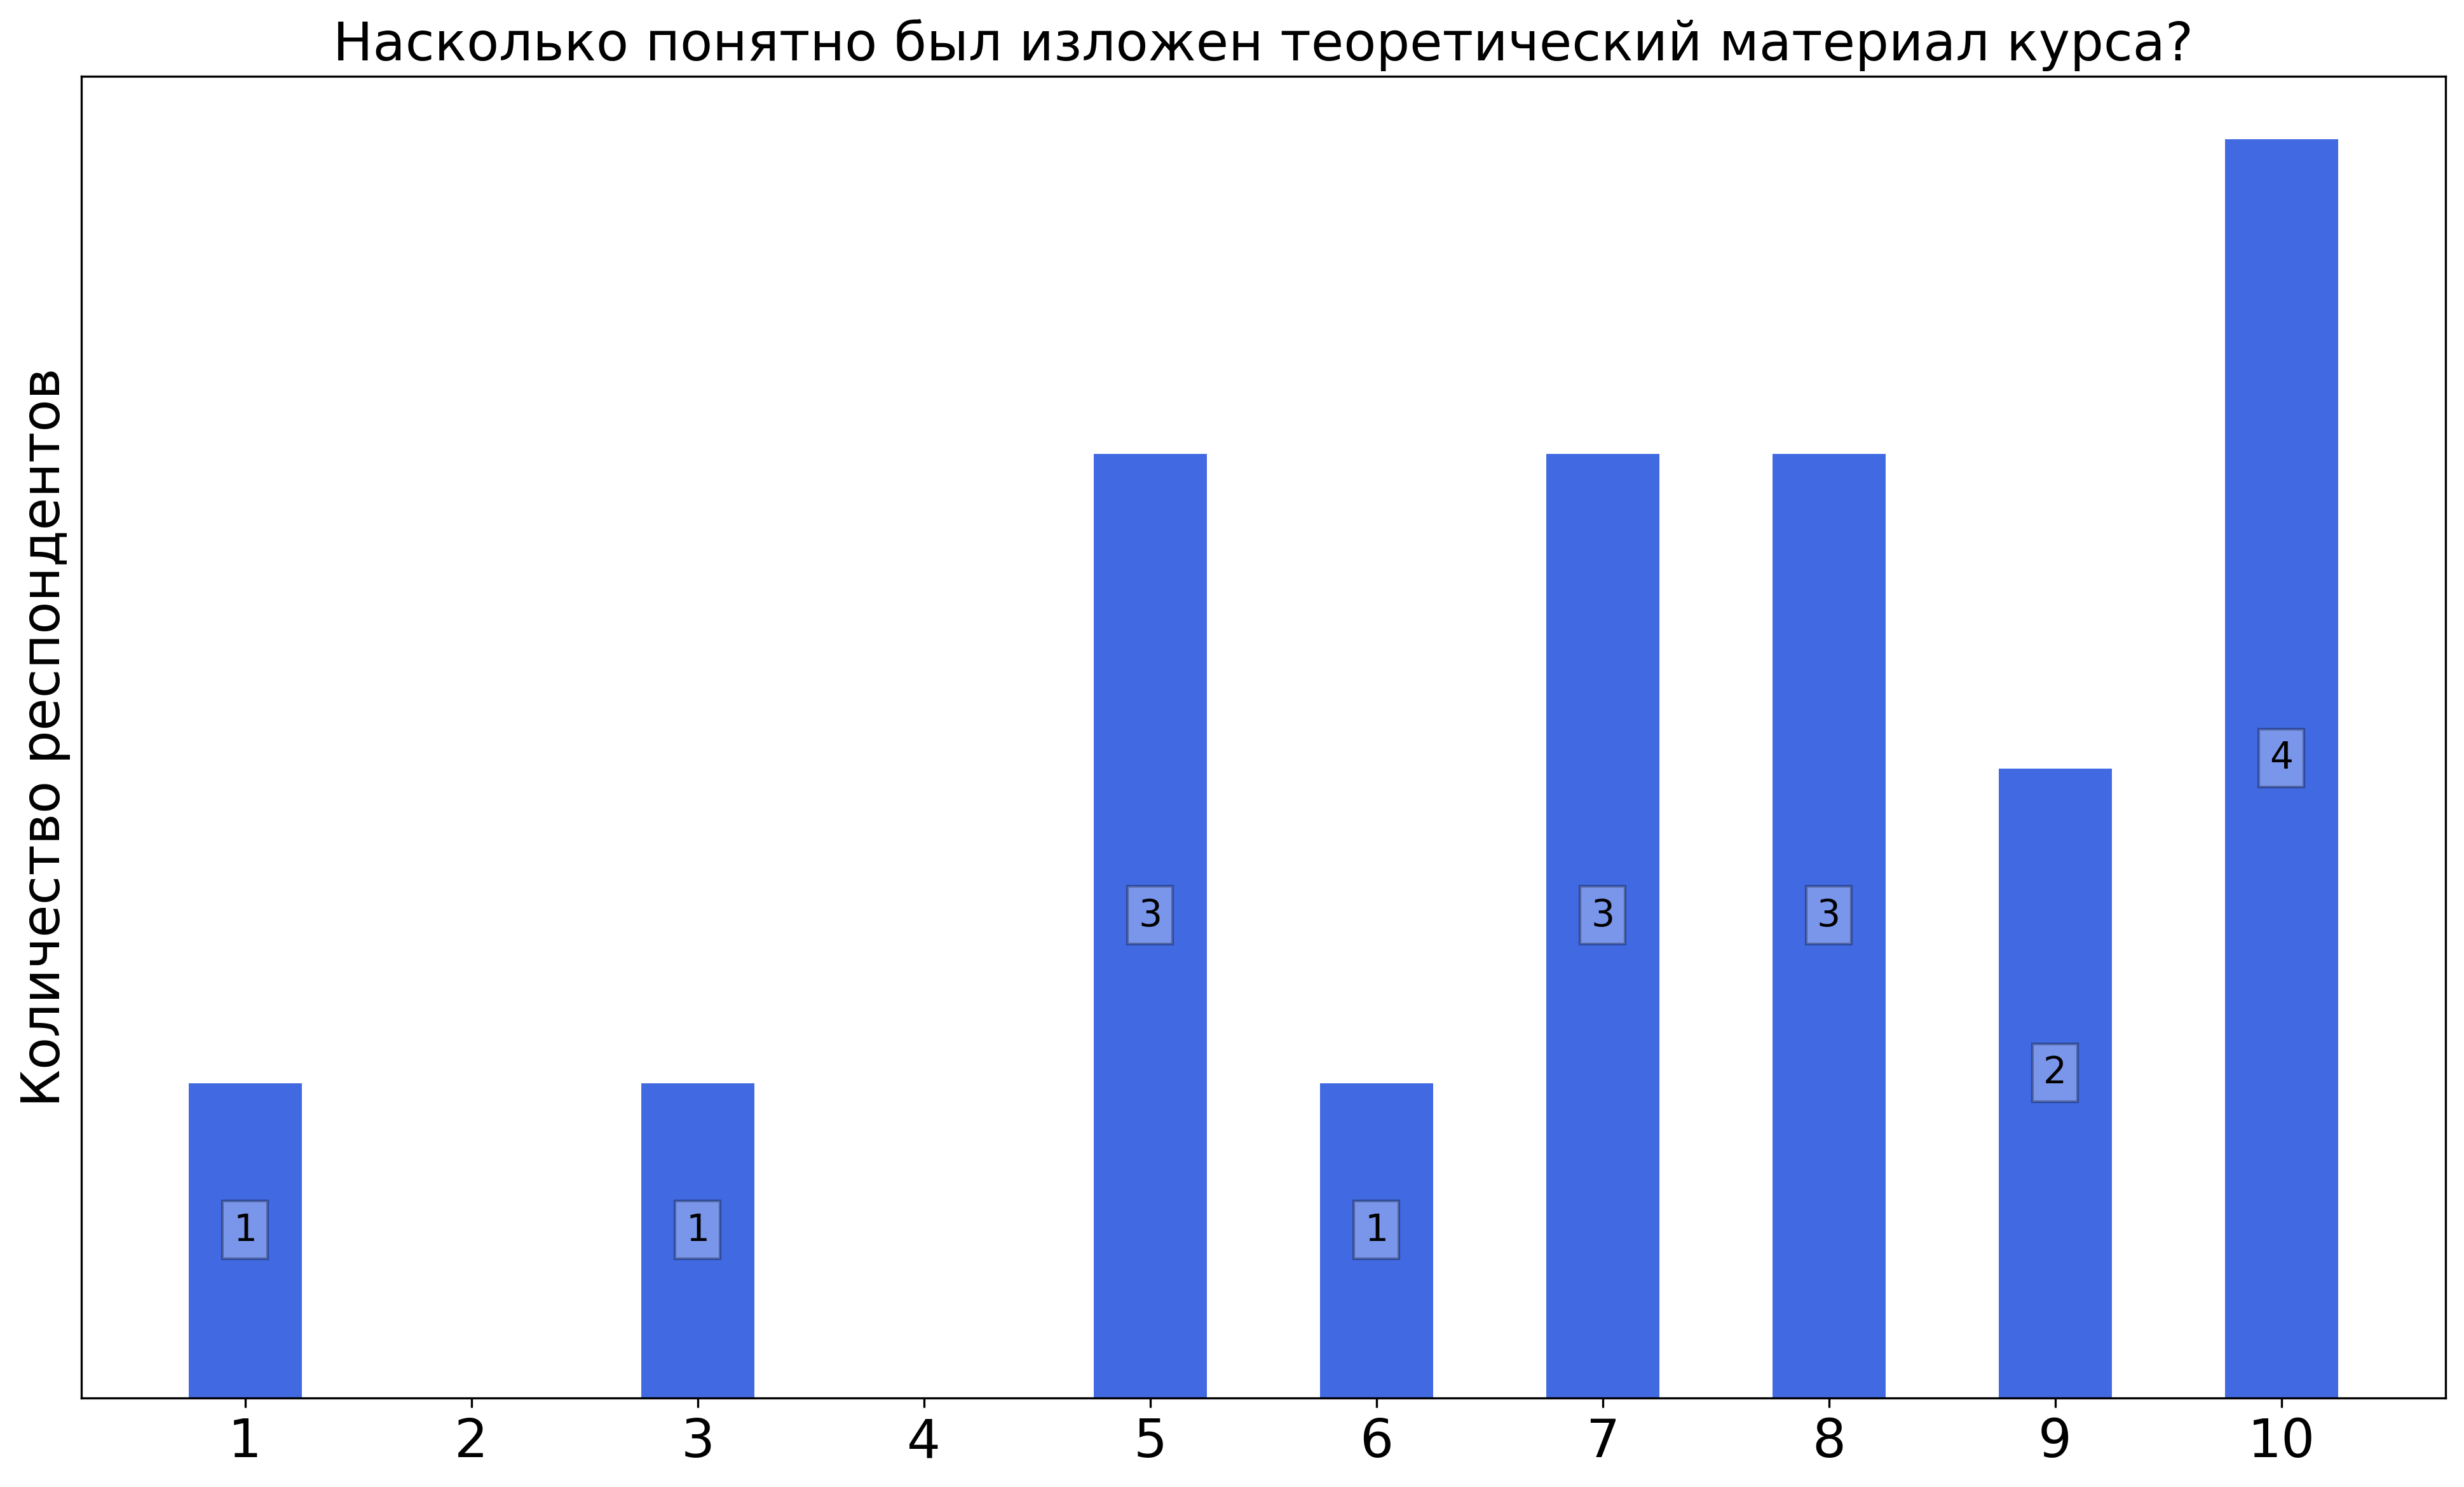
\includegraphics[width=\textwidth]{images/2 course/Дифференциальные уравнения/lecturer-marks-Бишаев А.М.-2.png}
			\end{subfigure}	
			\begin{subfigure}[b]{0.45\textwidth}
				\centering
				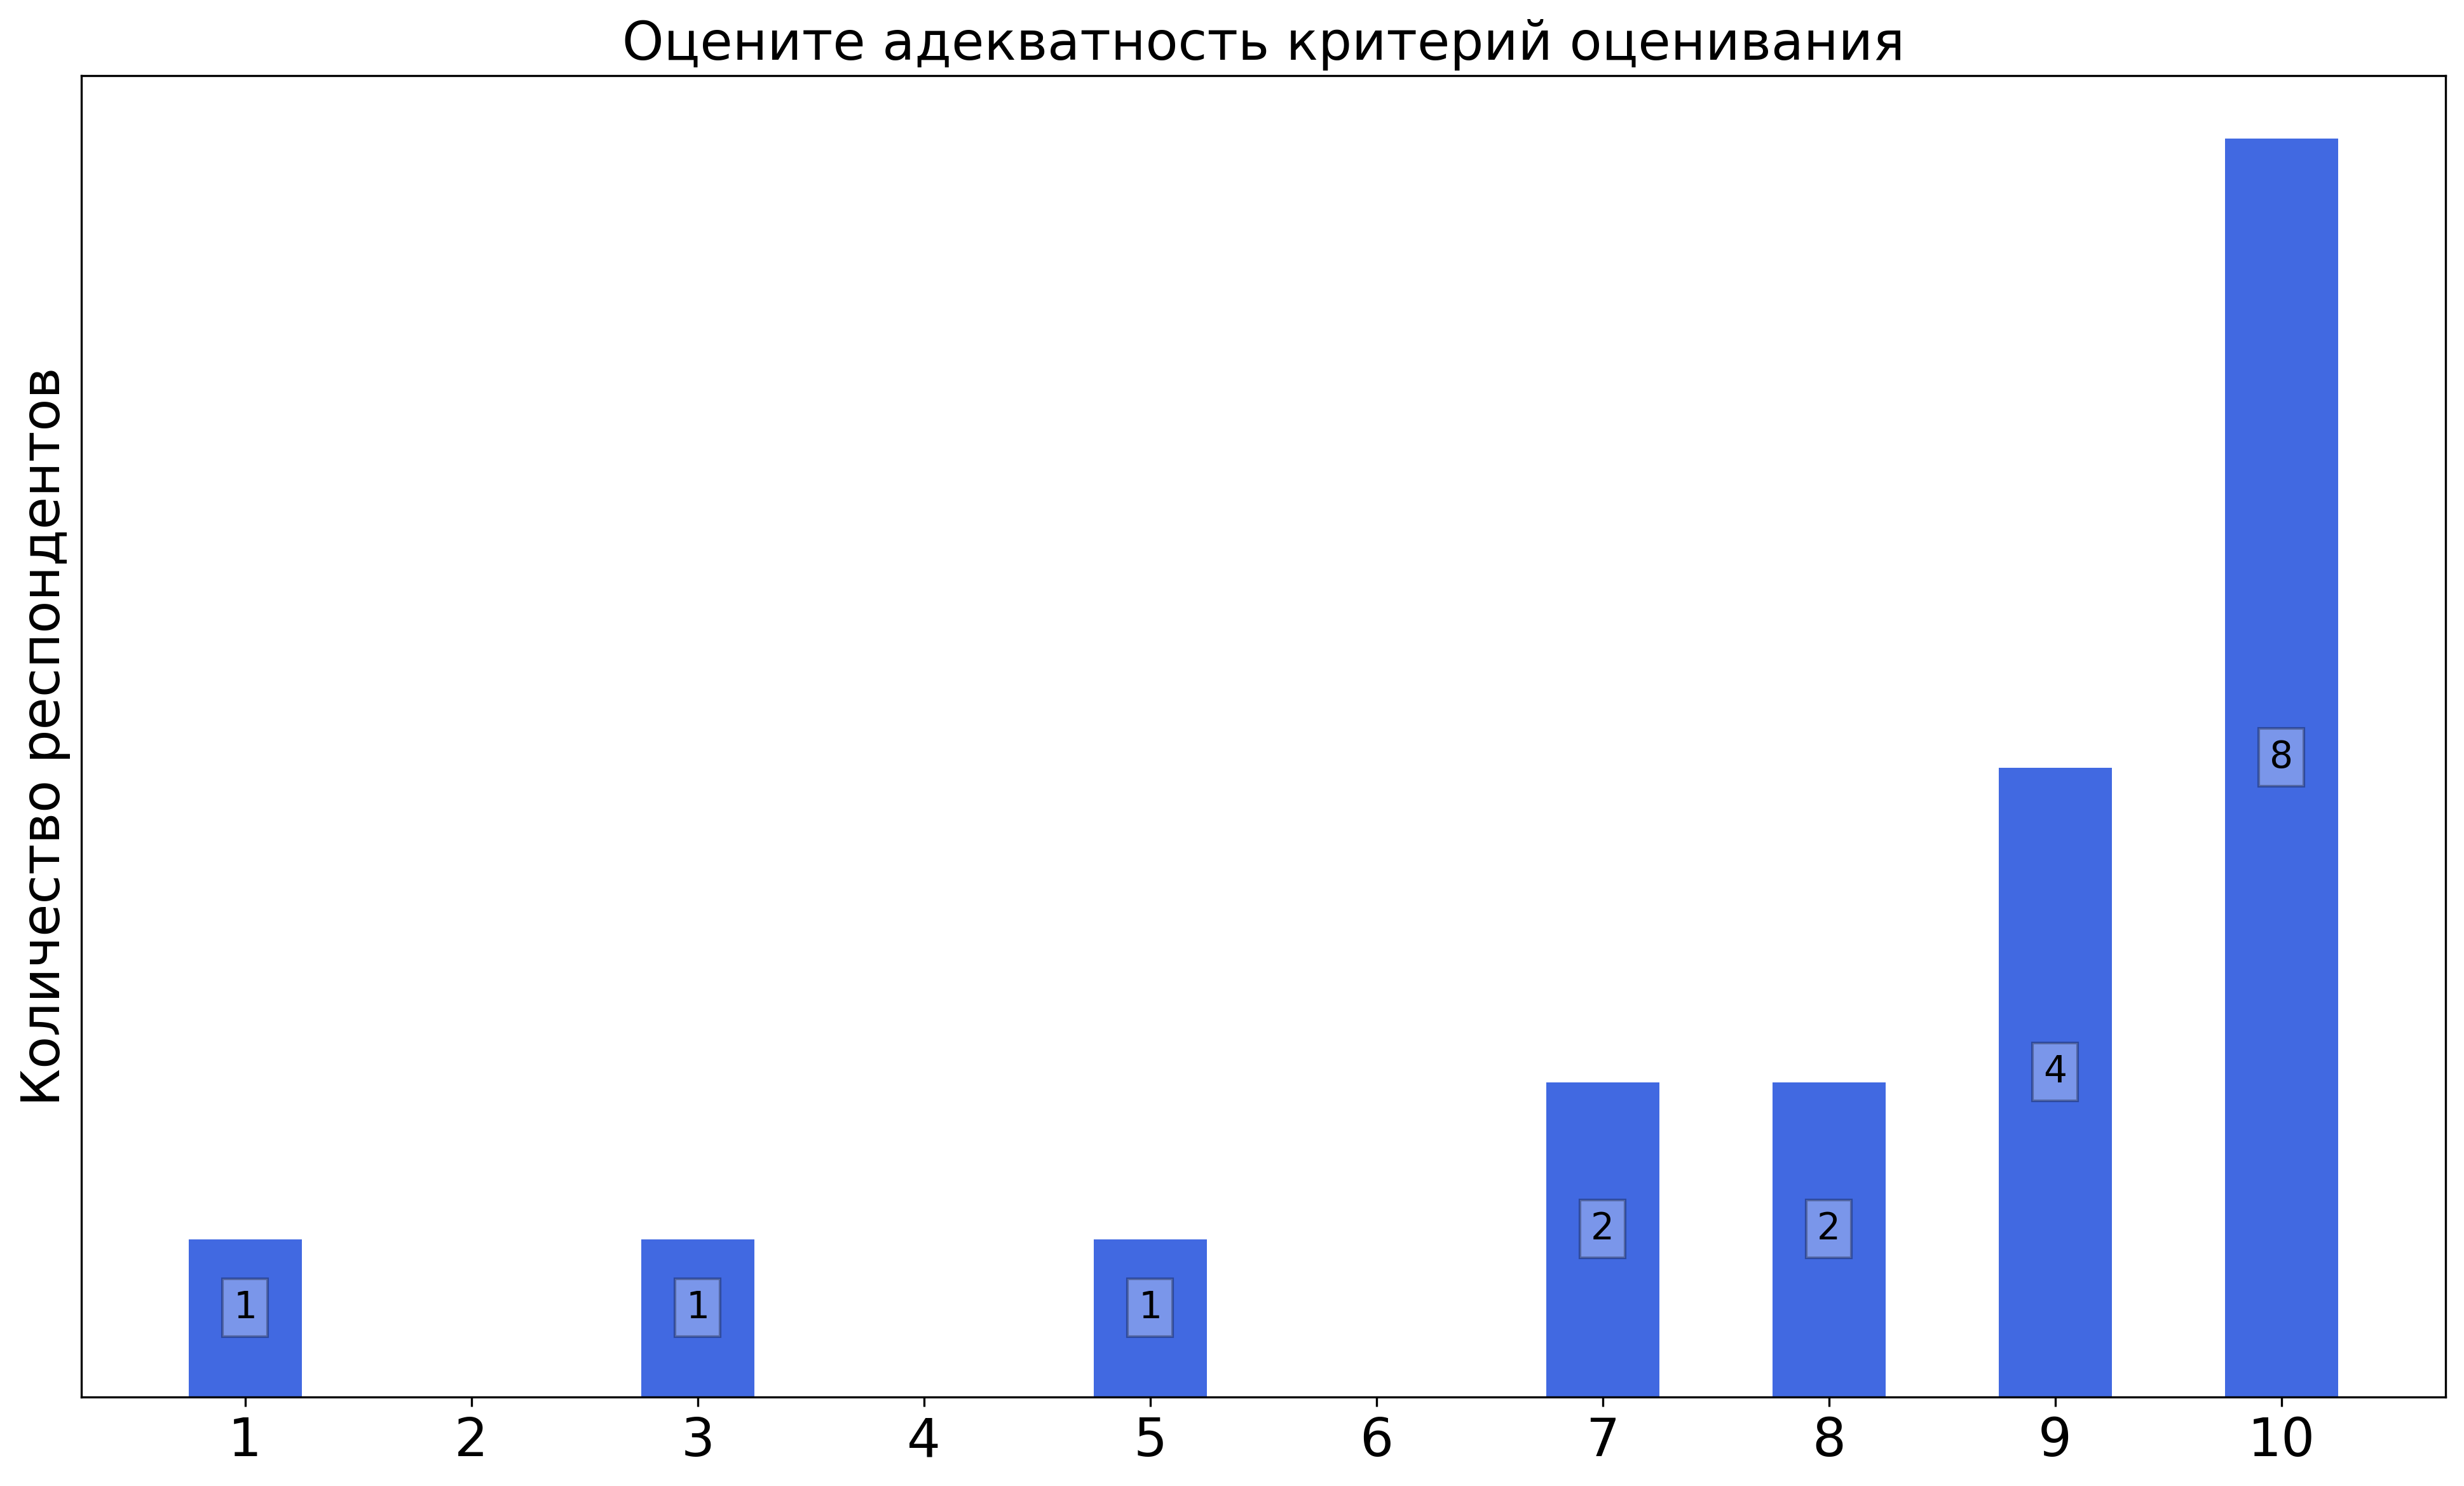
\includegraphics[width=\textwidth]{images/2 course/Дифференциальные уравнения/lecturer-marks-Бишаев А.М.-3.png}
			\end{subfigure}
			\caption{Оценки респондентов о качестве преподавания лекций по курсу <<Дифференциальные уравнения>>}
		\end{figure}

		\textbf{Комментарии студентов о лекциях\protect\footnote{сохранены оригинальные орфография и пунктуация}}
            \begin{commentbox} 
                Бишаев А.М. неплохой преподаватель, но предполагаю, что в силу возраста его лекции не совсем понятны
                Он читает медленно и допускает немалое количество ошибок 
            \end{commentbox} 
    
    
    \subsubsection{Отзыв студентов о семинарах. Семинарист: Барабанщиков А.В.}
		\begin{figure}[H]
			\centering
			\begin{subfigure}[b]{0.45\textwidth}
				\centering
				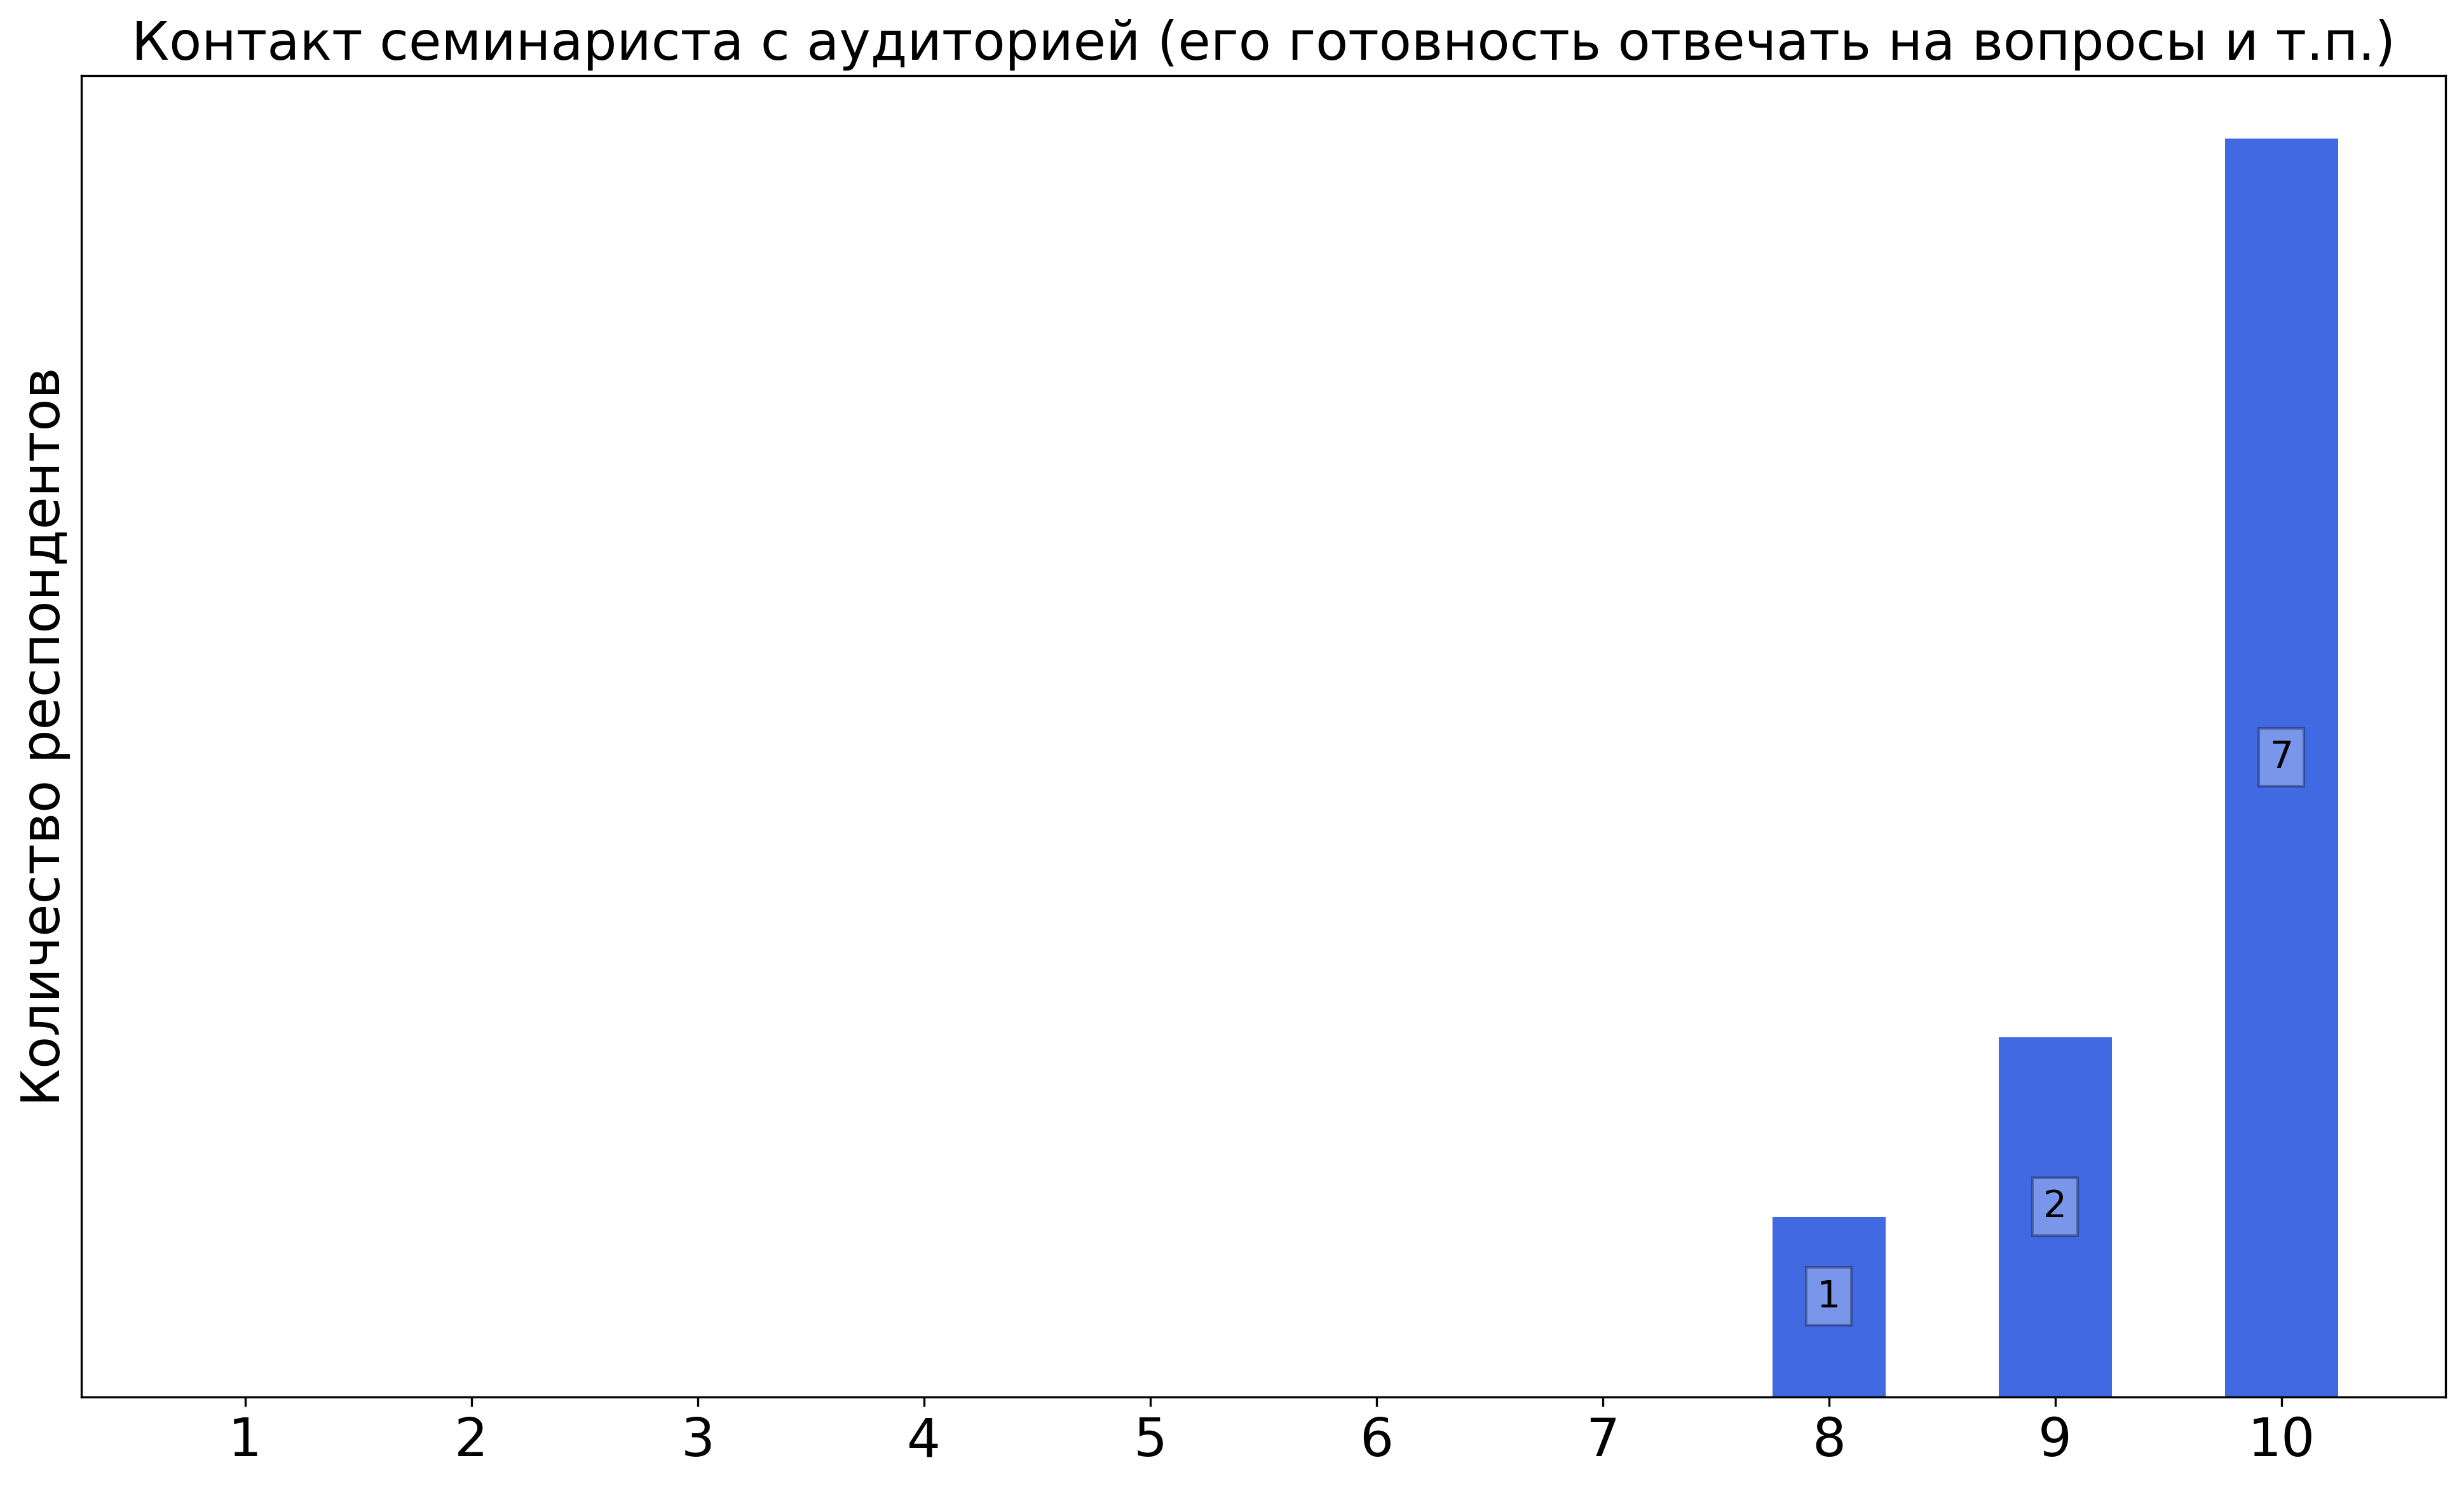
\includegraphics[width=\textwidth]{images/2 course/Дифференциальные уравнения/seminarists-marks-Барабанщиков А.В.-0.png}
			\end{subfigure}
			\begin{subfigure}[b]{0.45\textwidth}
				\centering
				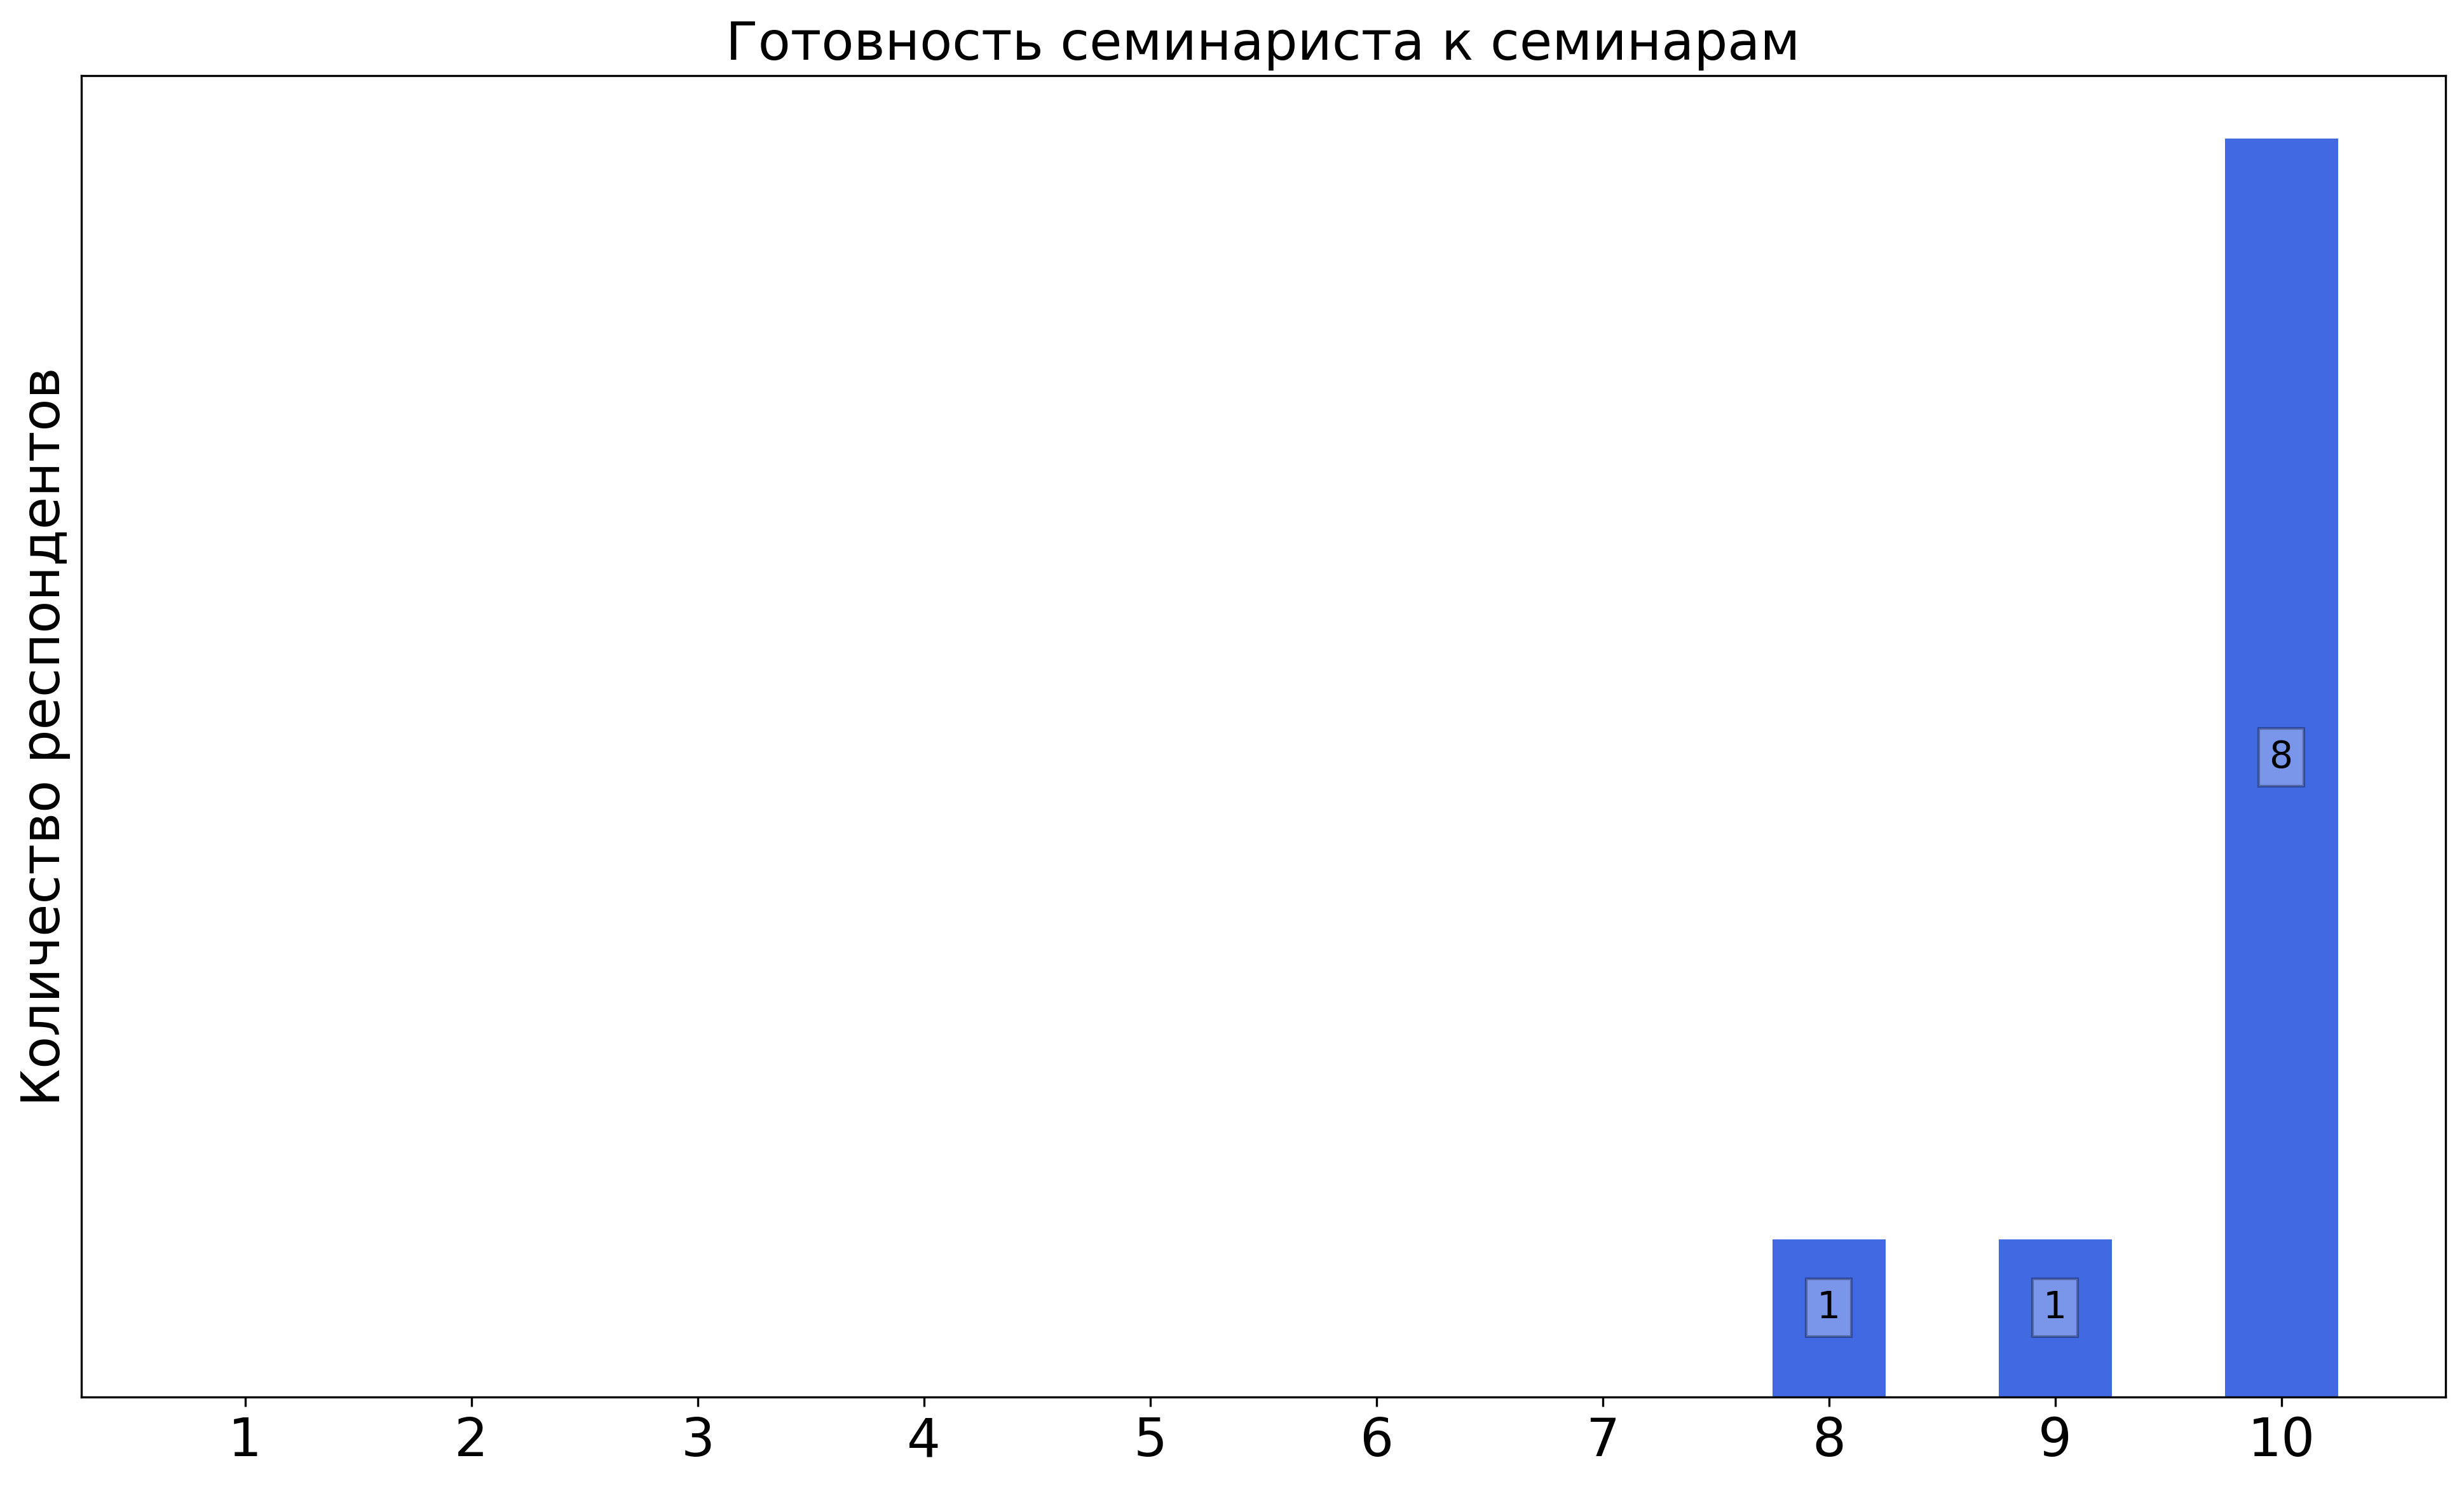
\includegraphics[width=\textwidth]{images/2 course/Дифференциальные уравнения/seminarists-marks-Барабанщиков А.В.-1.png}
			\end{subfigure}
			\begin{subfigure}[b]{0.45\textwidth}
				\centering
				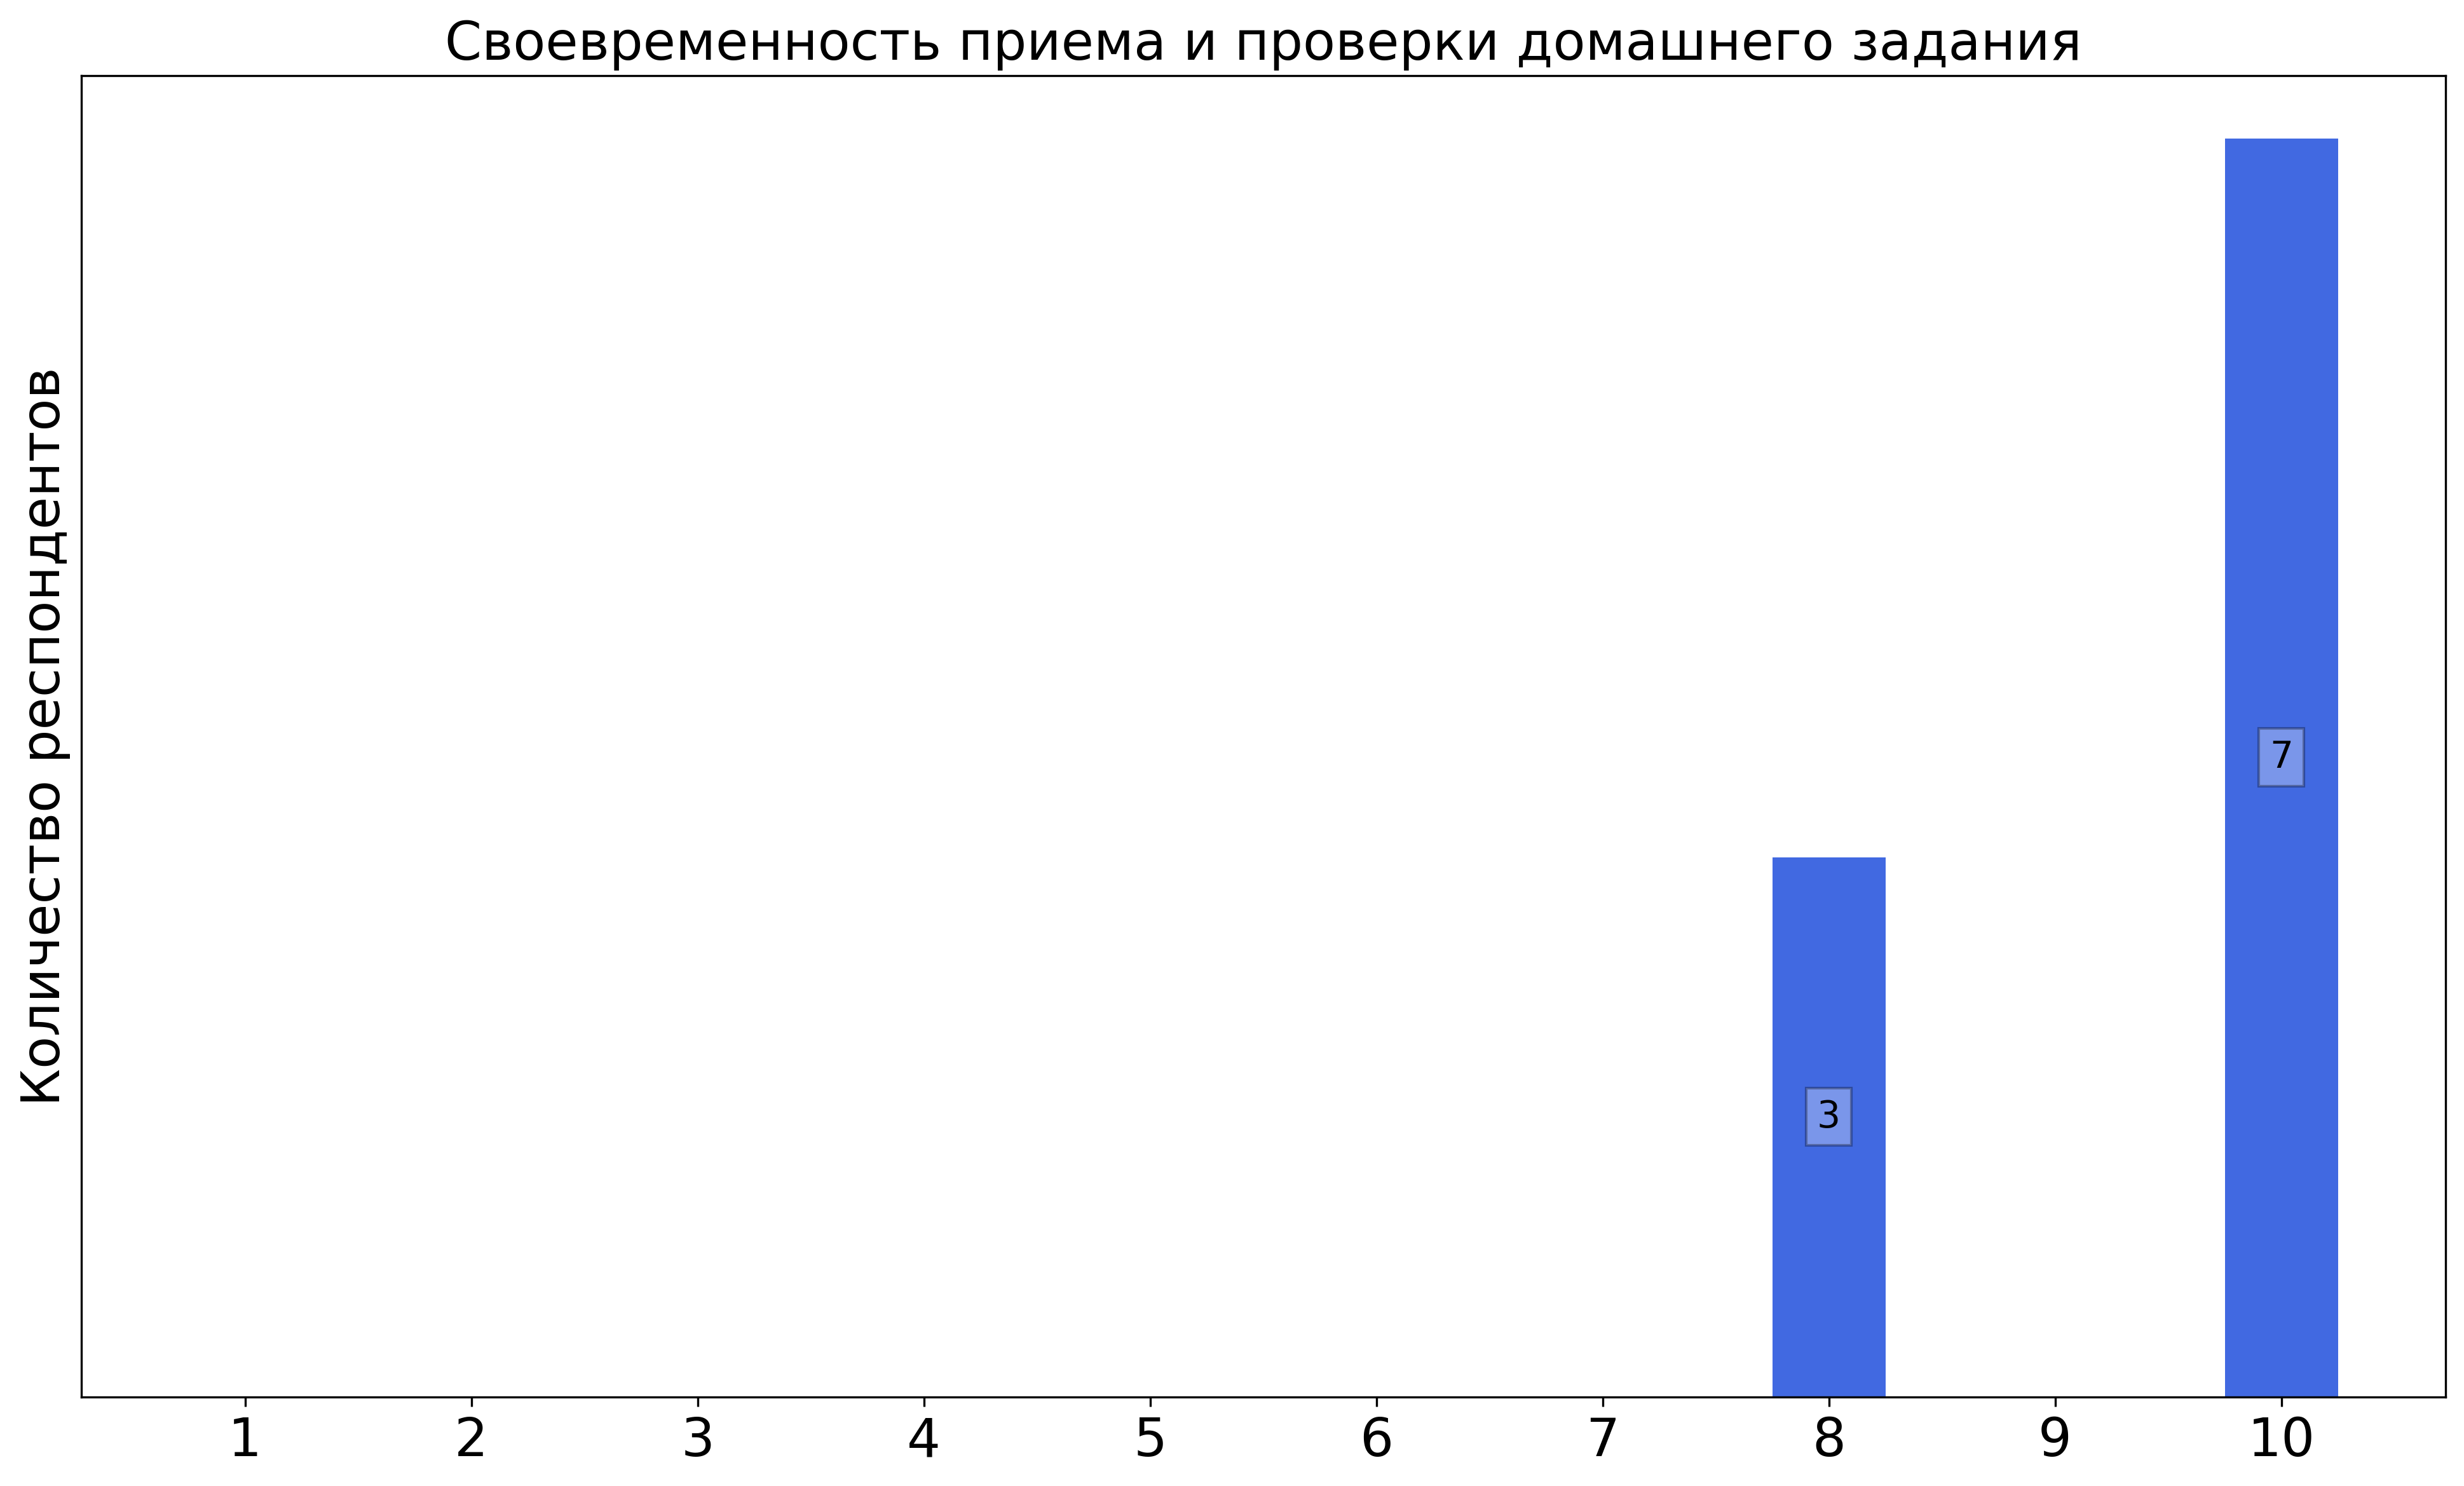
\includegraphics[width=\textwidth]{images/2 course/Дифференциальные уравнения/seminarists-marks-Барабанщиков А.В.-2.png}
			\end{subfigure}
			\begin{subfigure}[b]{0.45\textwidth}
				\centering
				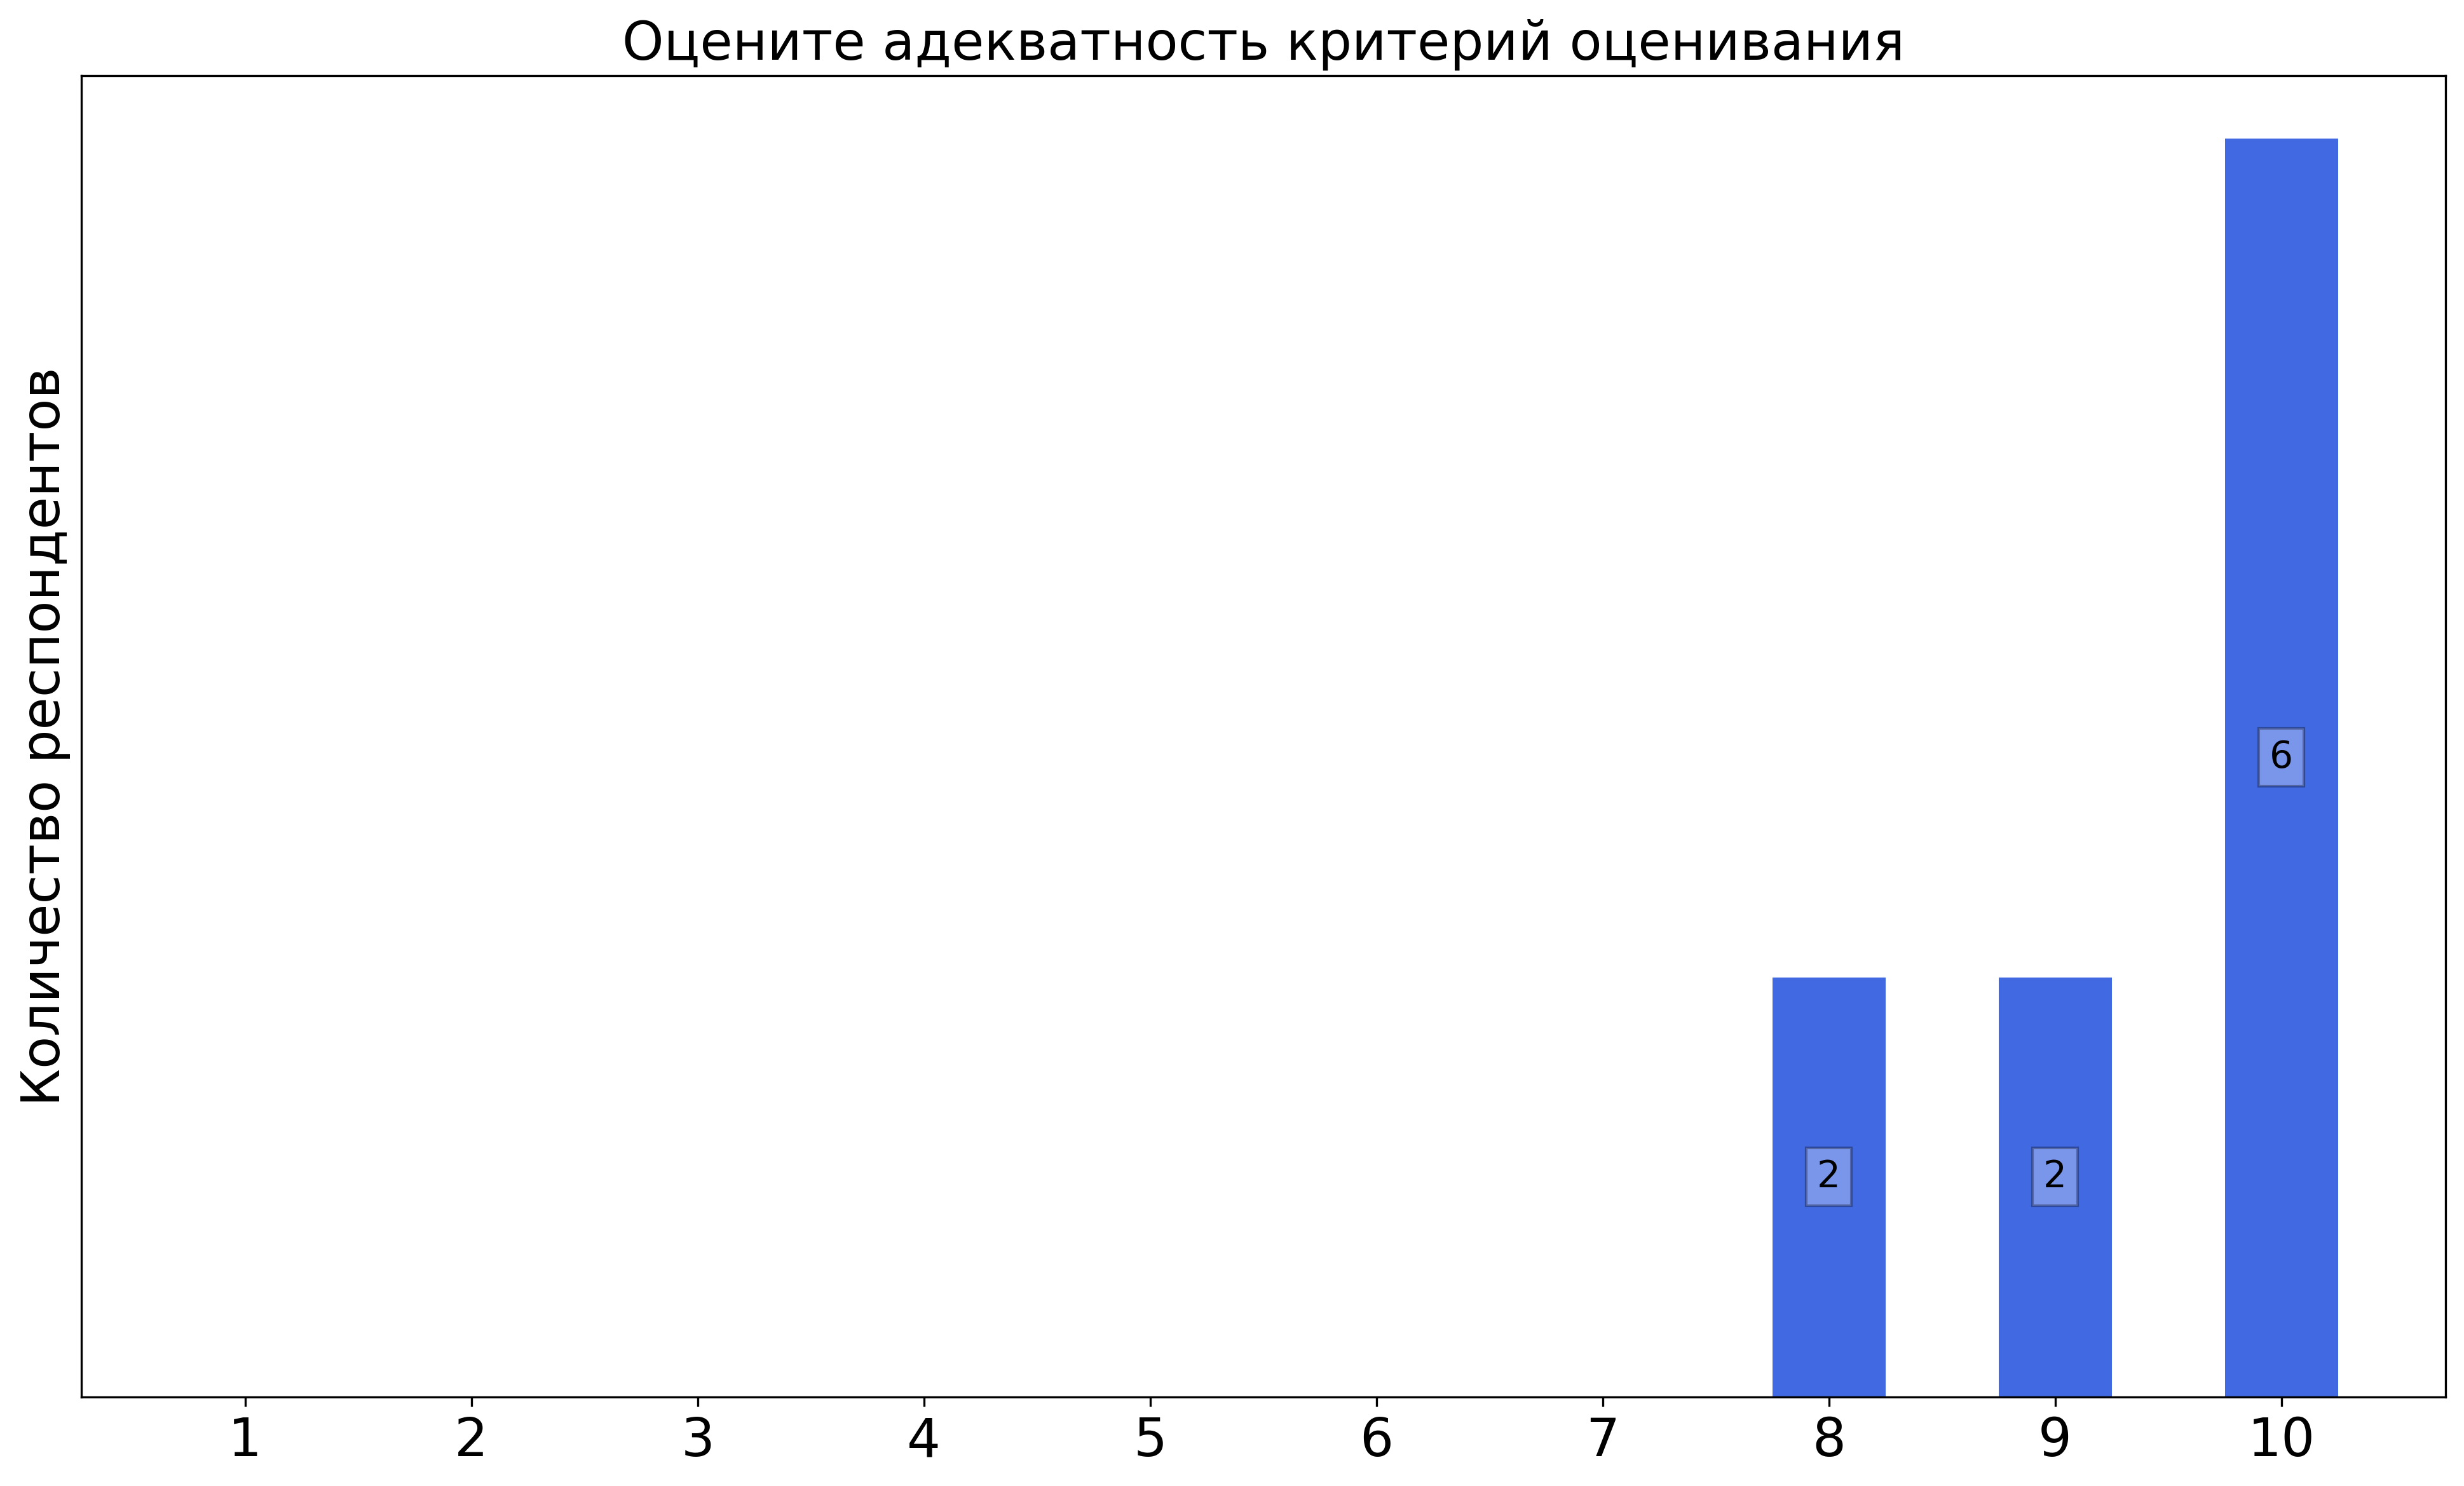
\includegraphics[width=\textwidth]{images/2 course/Дифференциальные уравнения/seminarists-marks-Барабанщиков А.В.-3.png}
			\end{subfigure}	
			\caption{Оценки респондентов о качестве преподавания семинаров}
		\end{figure}

		\textbf{Комментарии студентов о семинаристе\protect\footnote{сохранены оригинальные орфография и пунктуация}}
            \begin{commentbox} 
                Было полезно посещать занятия, но некоторые темы требовали больше времени для индивидуального освоения 
            \end{commentbox} 
        
        
    \subsubsection{Отзыв студентов о семинарах. Семинарист: Бишаев А.М.}
		\begin{figure}[H]
			\centering
			\begin{subfigure}[b]{0.45\textwidth}
				\centering
				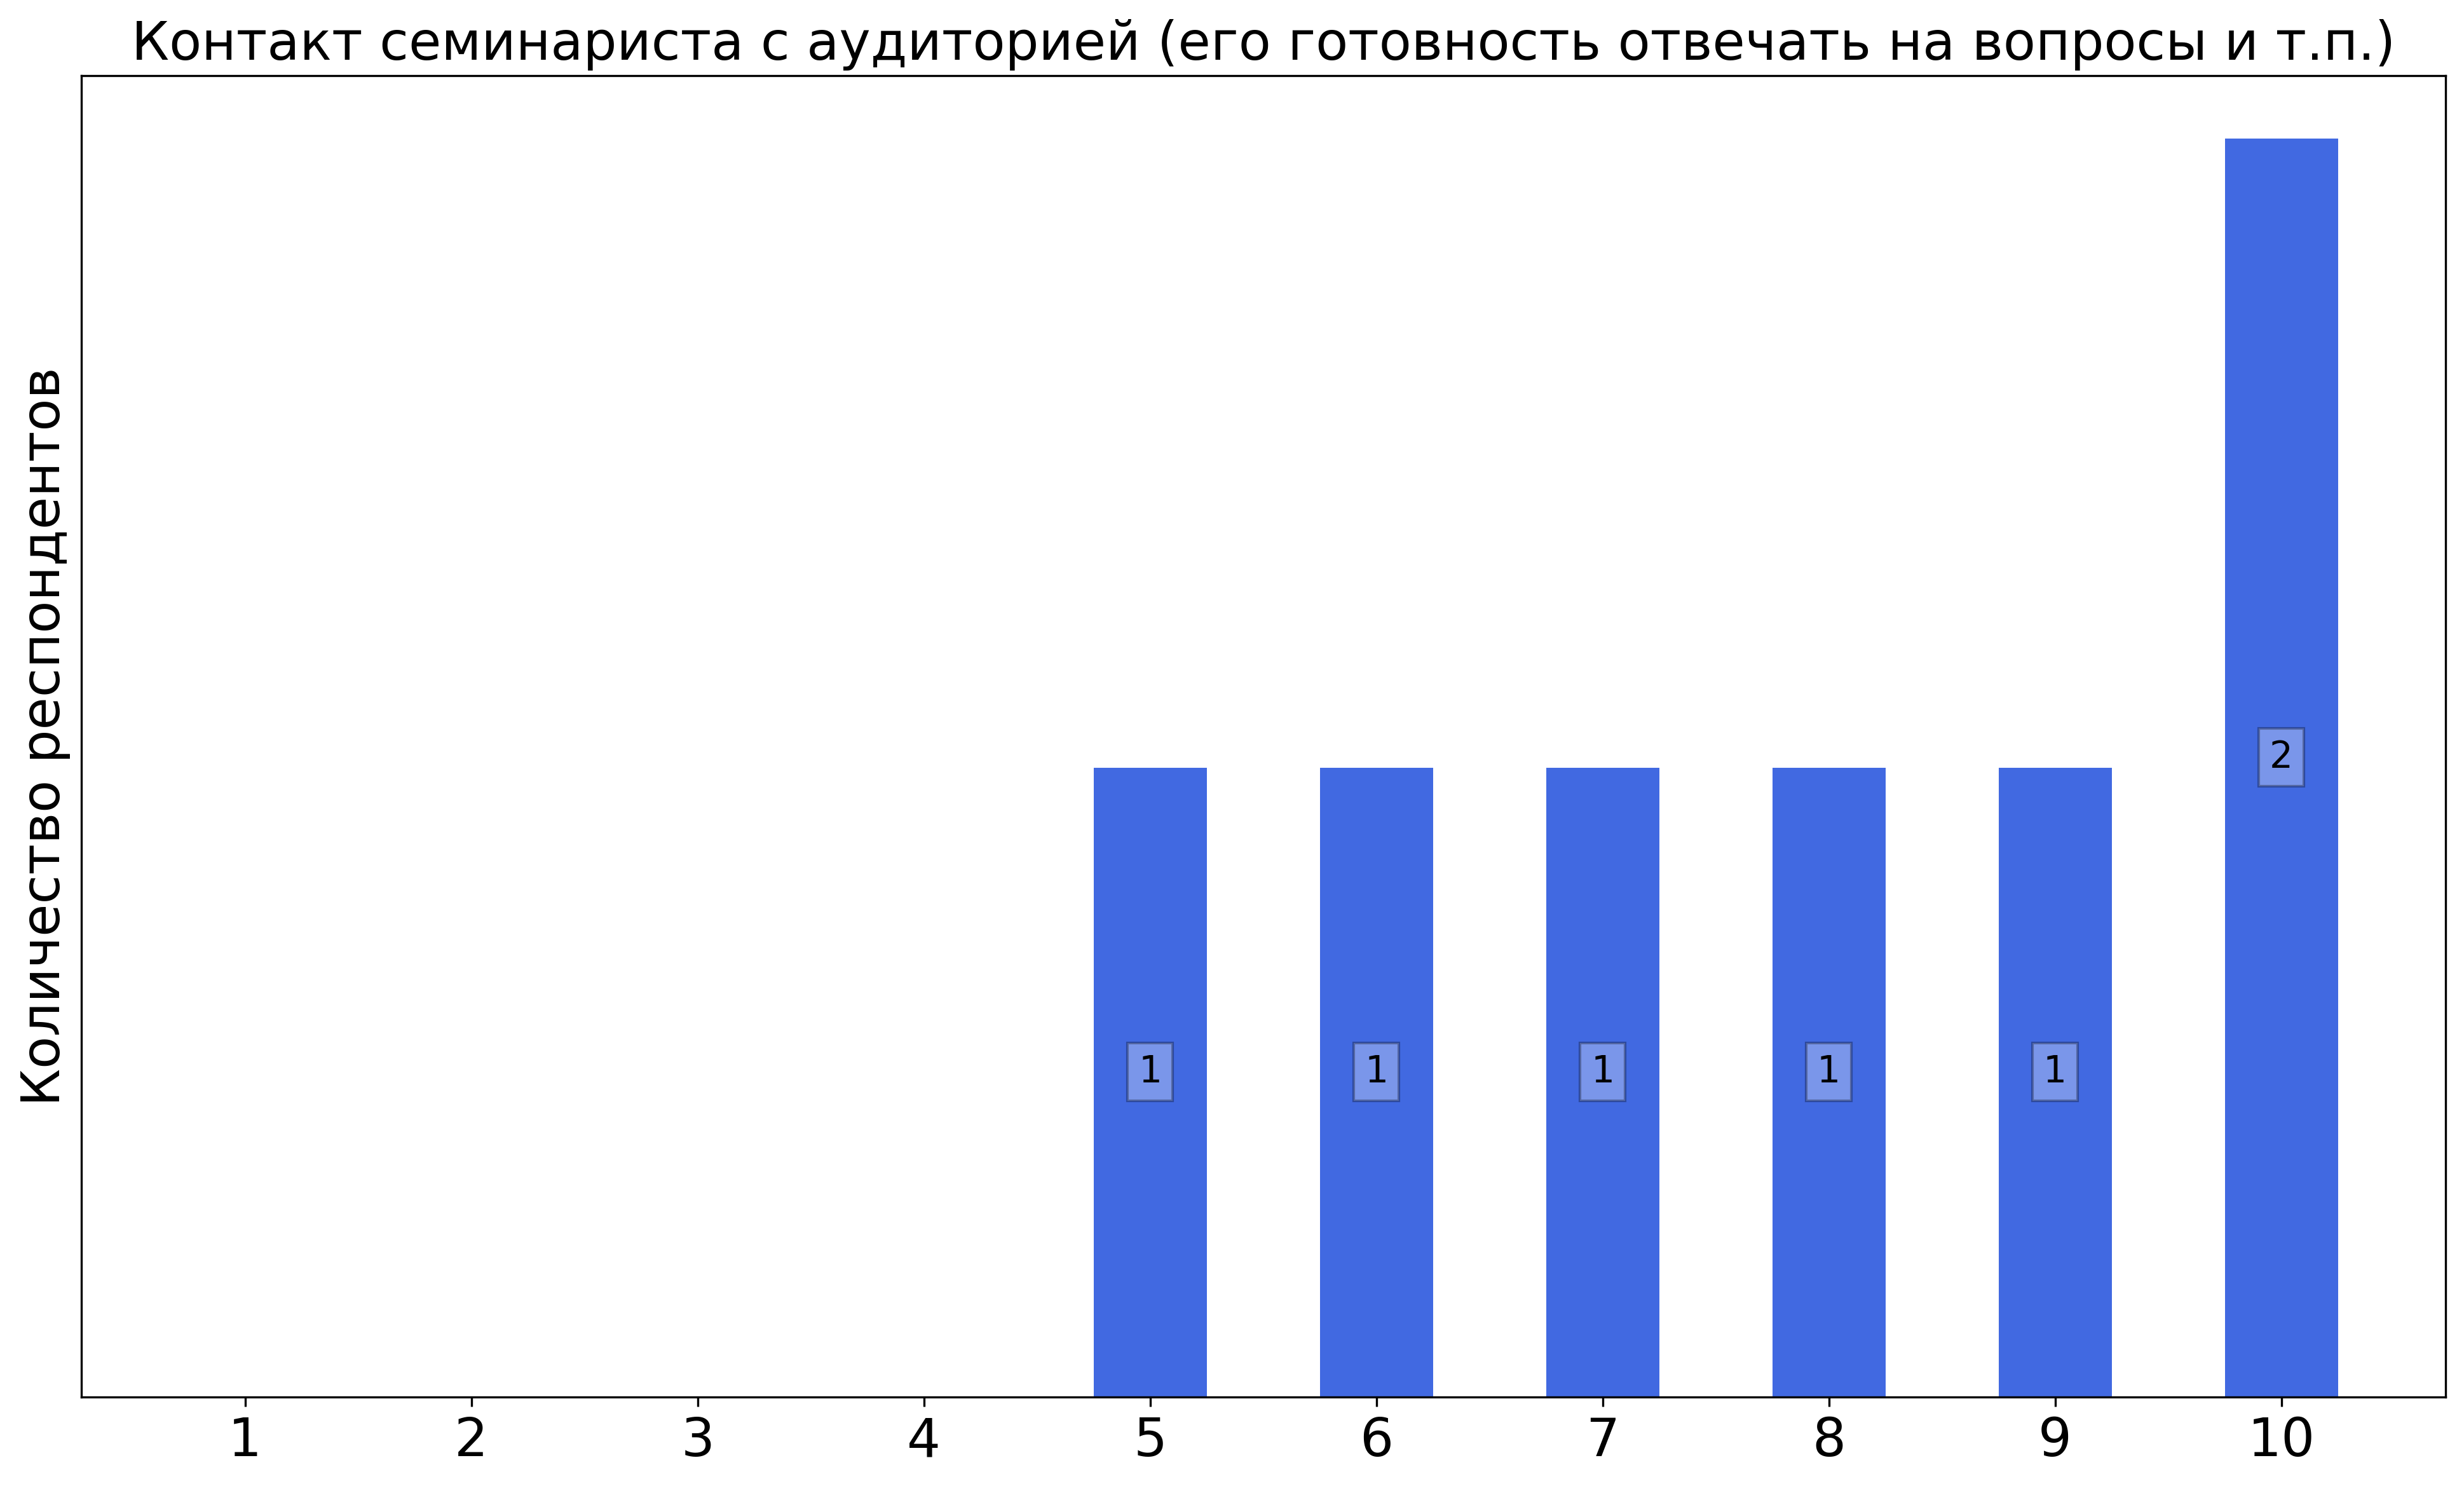
\includegraphics[width=\textwidth]{images/2 course/Дифференциальные уравнения/seminarists-marks-Бишаев А.М.-0.png}
			\end{subfigure}
			\begin{subfigure}[b]{0.45\textwidth}
				\centering
				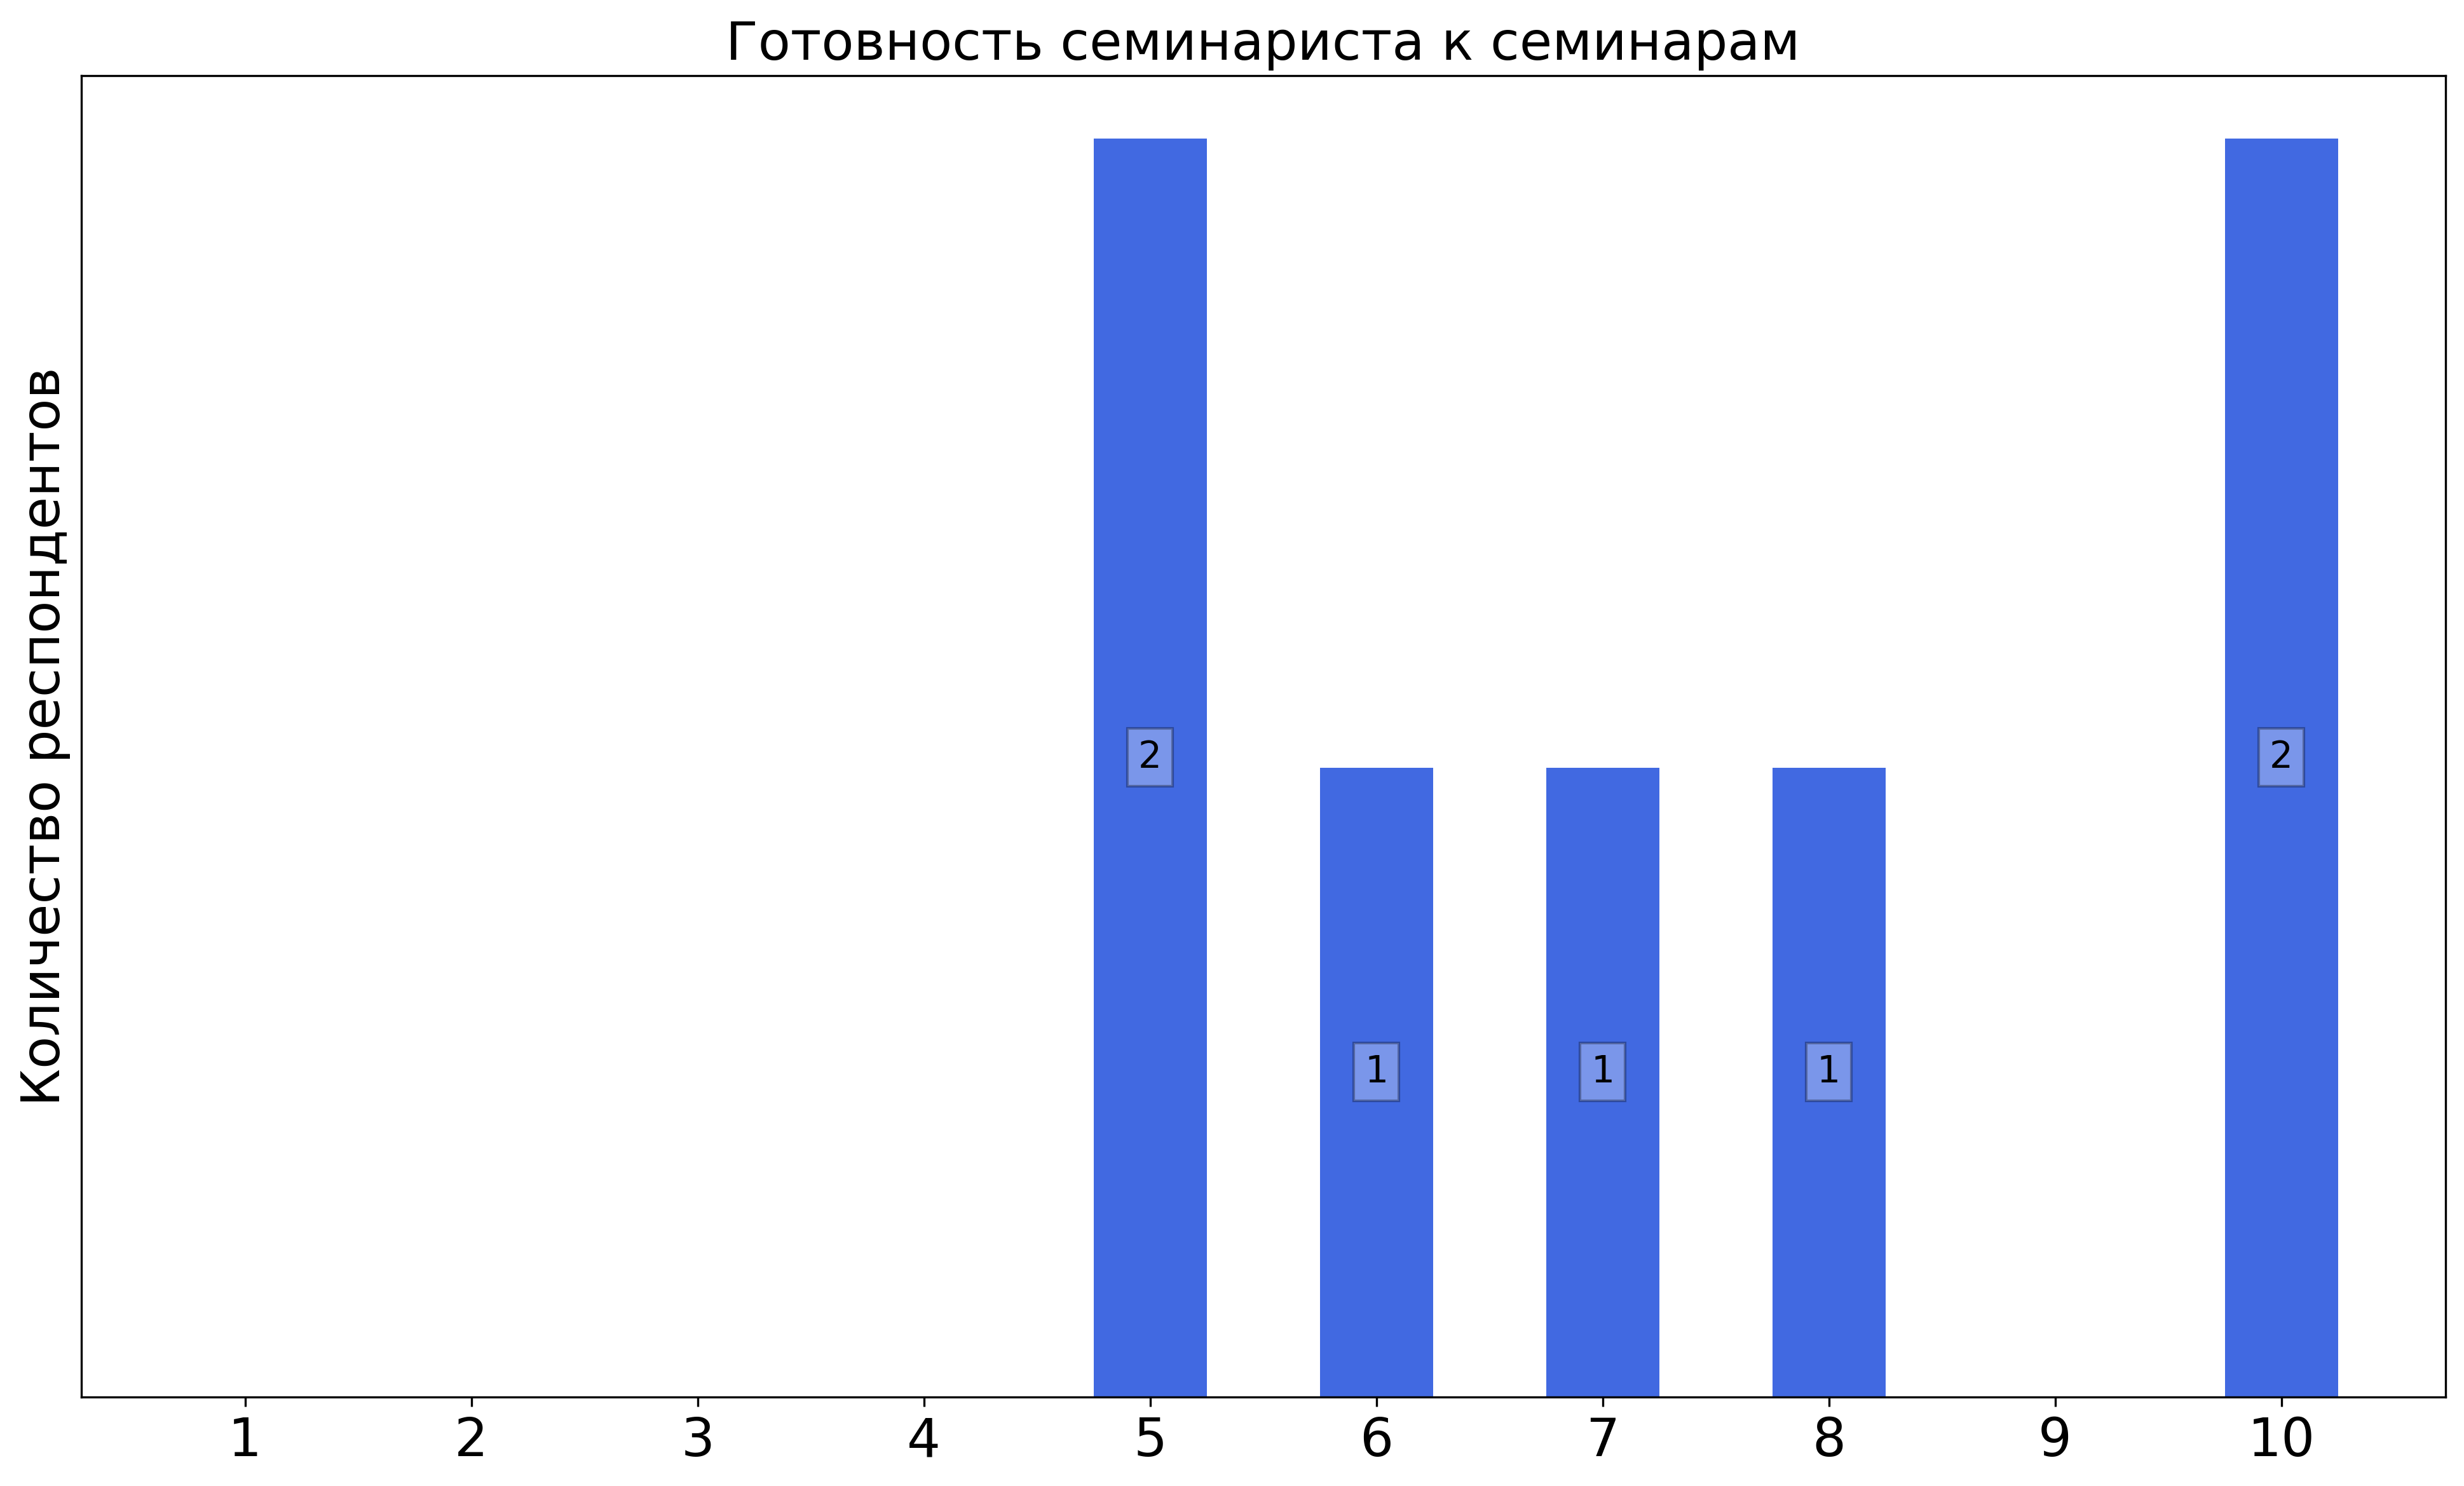
\includegraphics[width=\textwidth]{images/2 course/Дифференциальные уравнения/seminarists-marks-Бишаев А.М.-1.png}
			\end{subfigure}
			\begin{subfigure}[b]{0.45\textwidth}
				\centering
				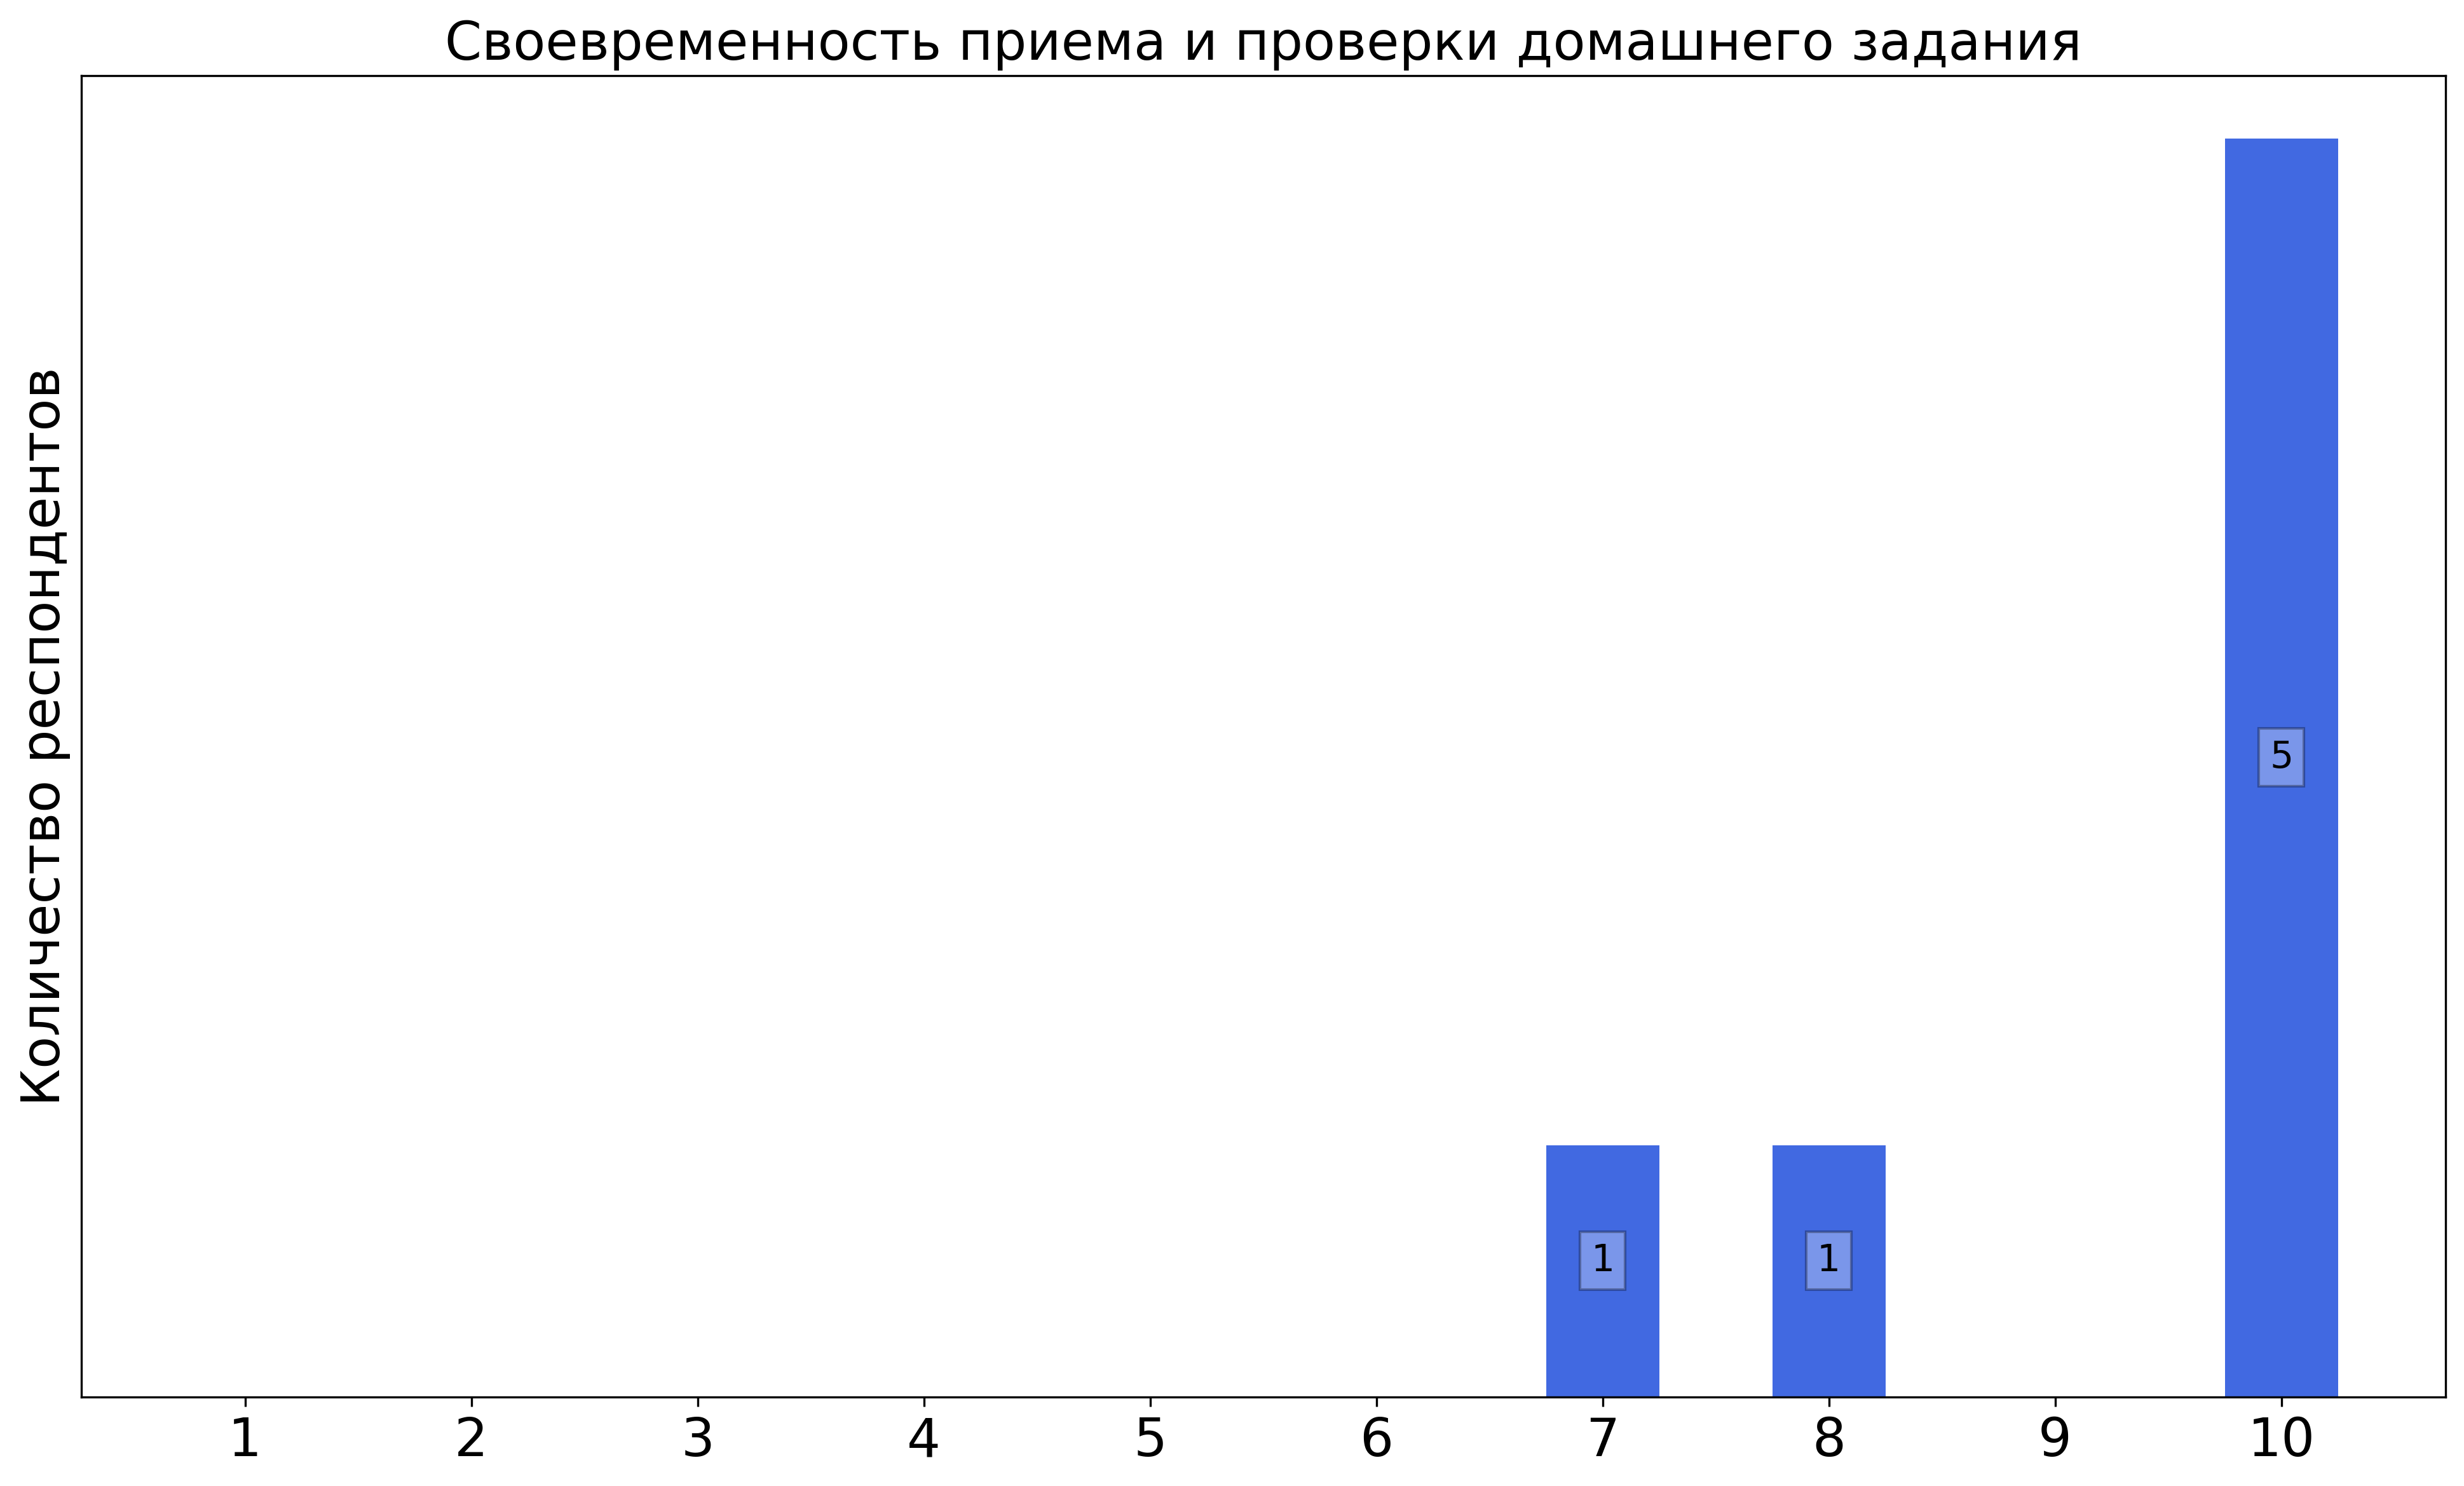
\includegraphics[width=\textwidth]{images/2 course/Дифференциальные уравнения/seminarists-marks-Бишаев А.М.-2.png}
			\end{subfigure}
			\begin{subfigure}[b]{0.45\textwidth}
				\centering
				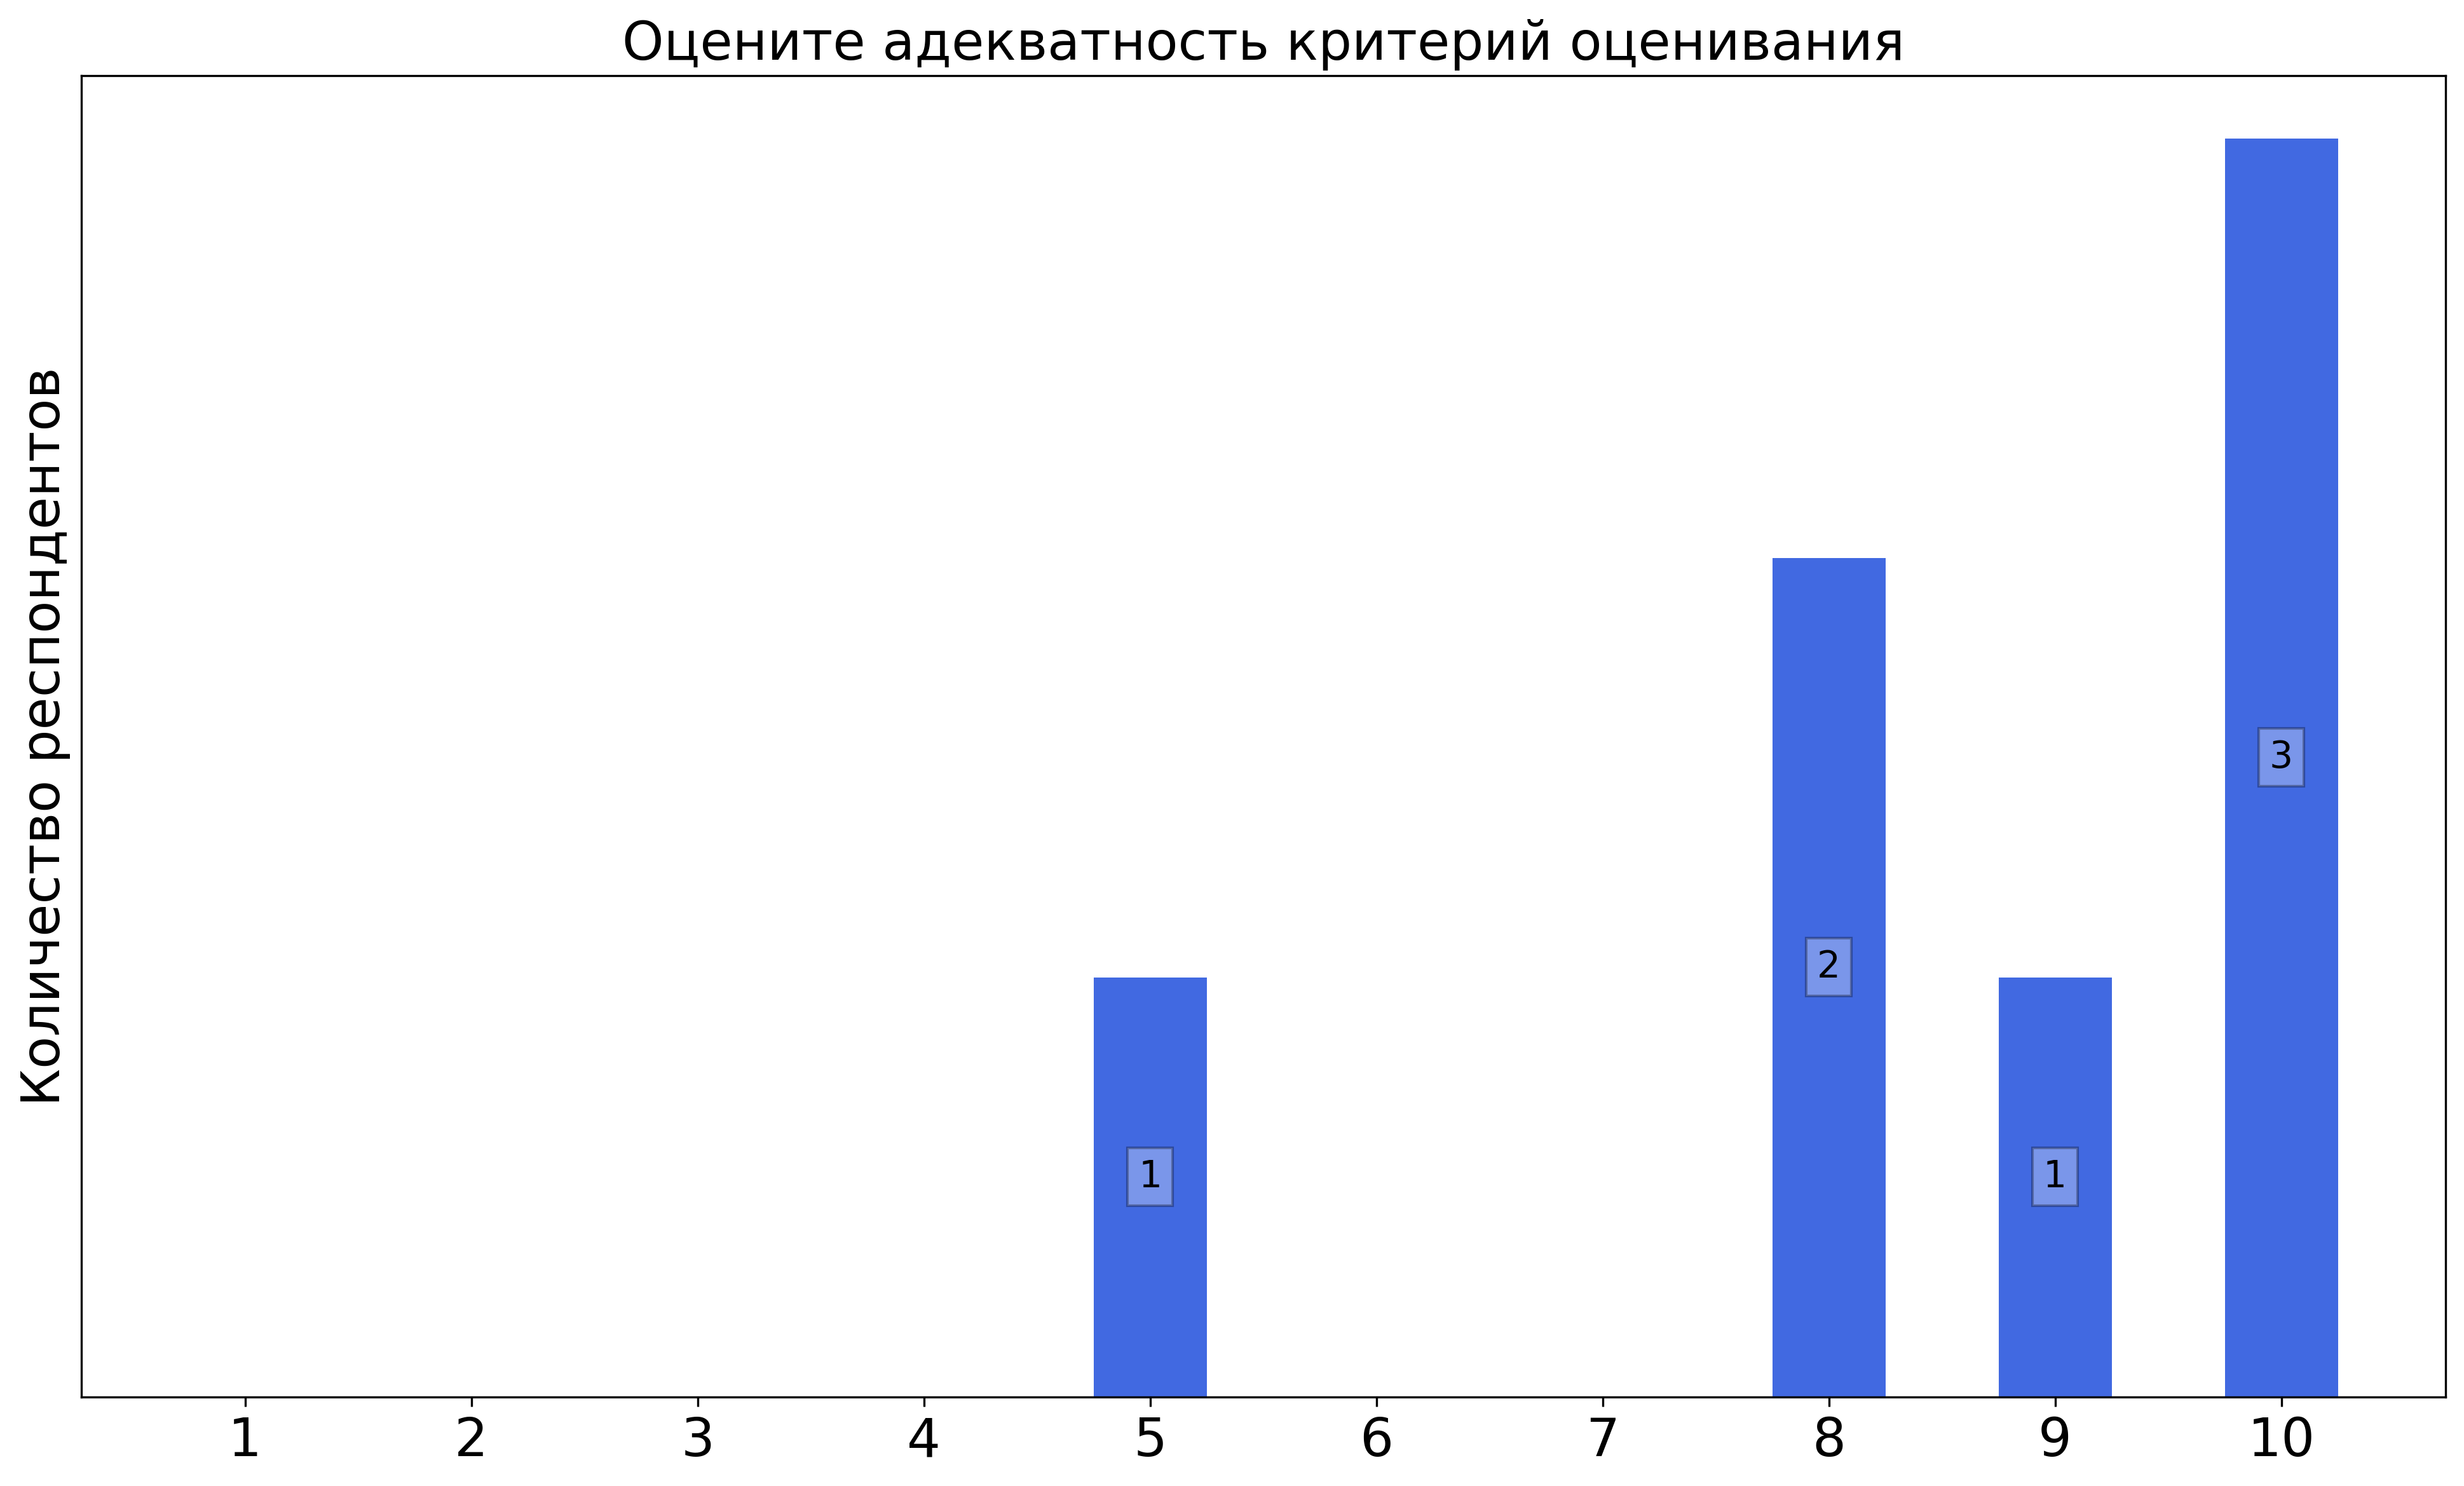
\includegraphics[width=\textwidth]{images/2 course/Дифференциальные уравнения/seminarists-marks-Бишаев А.М.-3.png}
			\end{subfigure}	
			\caption{Оценки респондентов о качестве преподавания семинаров}
		\end{figure}

		\textbf{Комментарии студентов о семинаристе\protect\footnote{сохранены оригинальные орфография и пунктуация}}
            \begin{commentbox} 
                Как семинарист Бишаев А.М. очень хороший
                Да, порой он тратит всю пару на решение одного уравнения, но скорее всего перед этим расскажет теорию и покажет несколько методов решения
                Контрольные и домашки проверяет во время и ставит оценки справедливо
                К итоговой оценке вопросов не имею 
            \end{commentbox} 
        
            \begin{commentbox} 
                Александр Михайлович достаточно специфично ведёт материал. Его часто приходится поправлять на ошибки, что не уменьшает количество проходимого материала  
            \end{commentbox}


    \subsubsection{Отзыв студентов о семинарах. Семинарист: Глухова Е.В.}
		\begin{figure}[H]
			\centering
			\begin{subfigure}[b]{0.45\textwidth}
				\centering
				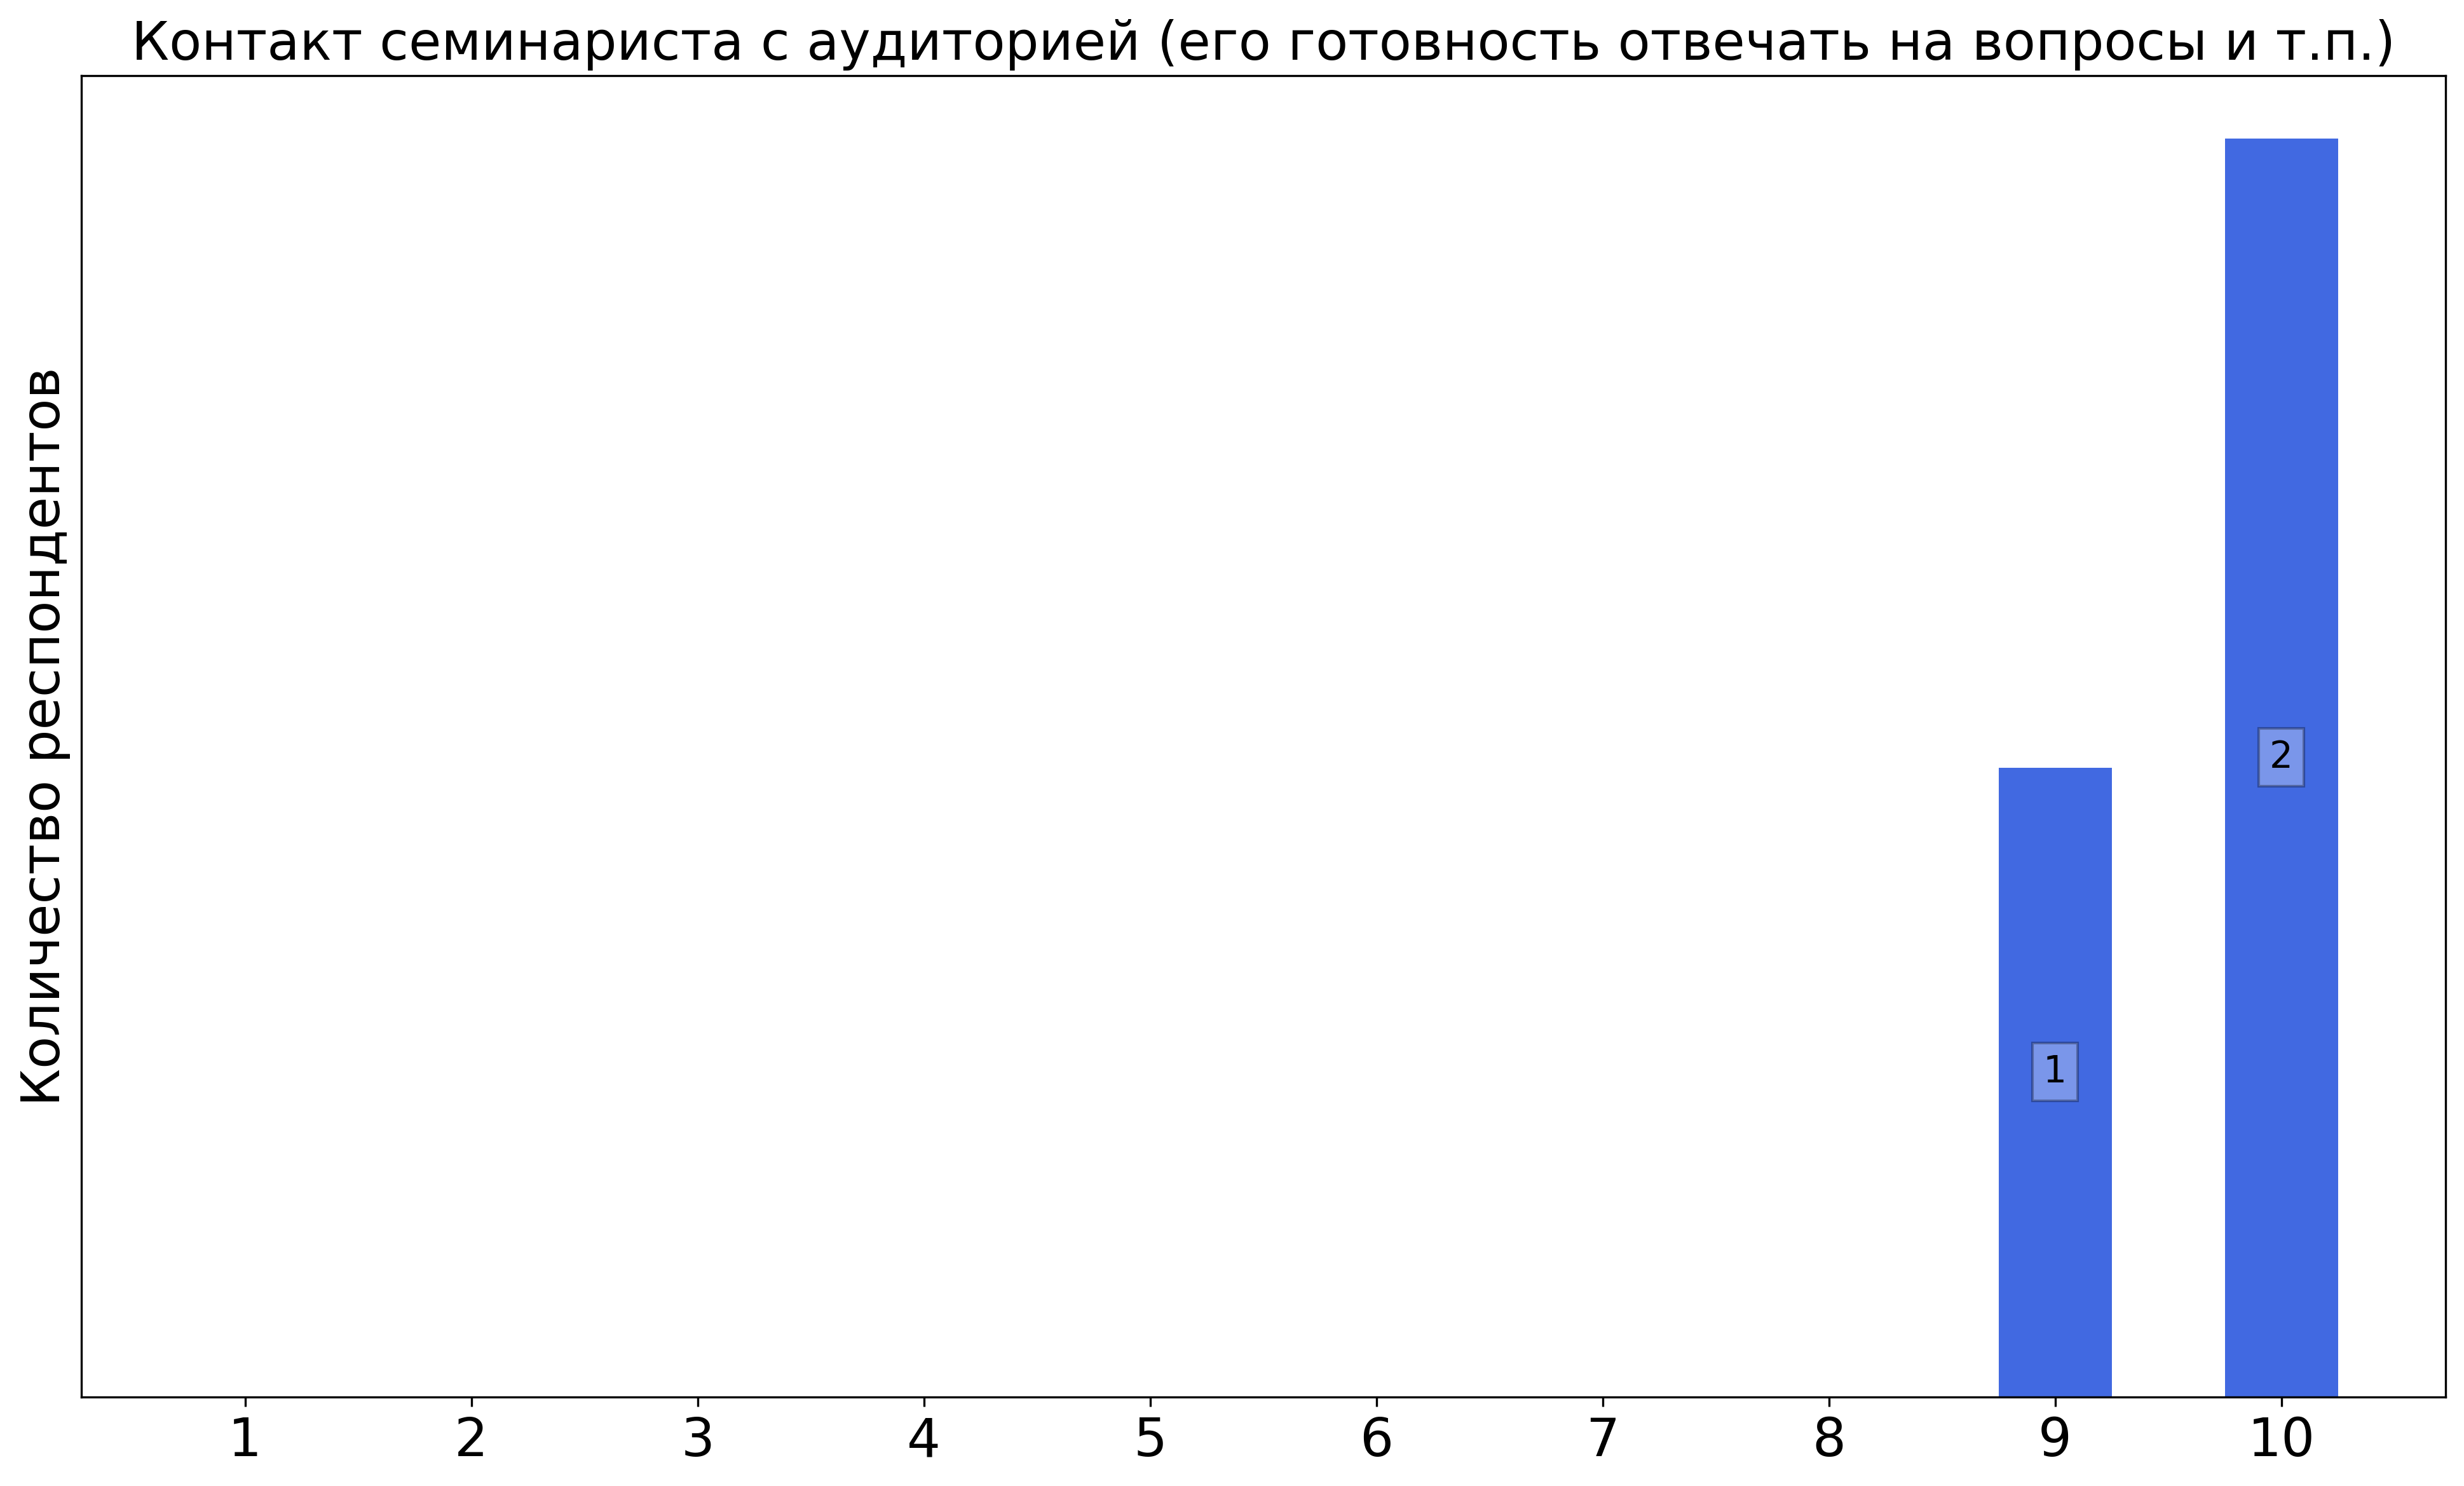
\includegraphics[width=\textwidth]{images/2 course/Дифференциальные уравнения/seminarists-marks-Глухова Е.В.-0.png}
			\end{subfigure}
			\begin{subfigure}[b]{0.45\textwidth}
				\centering
				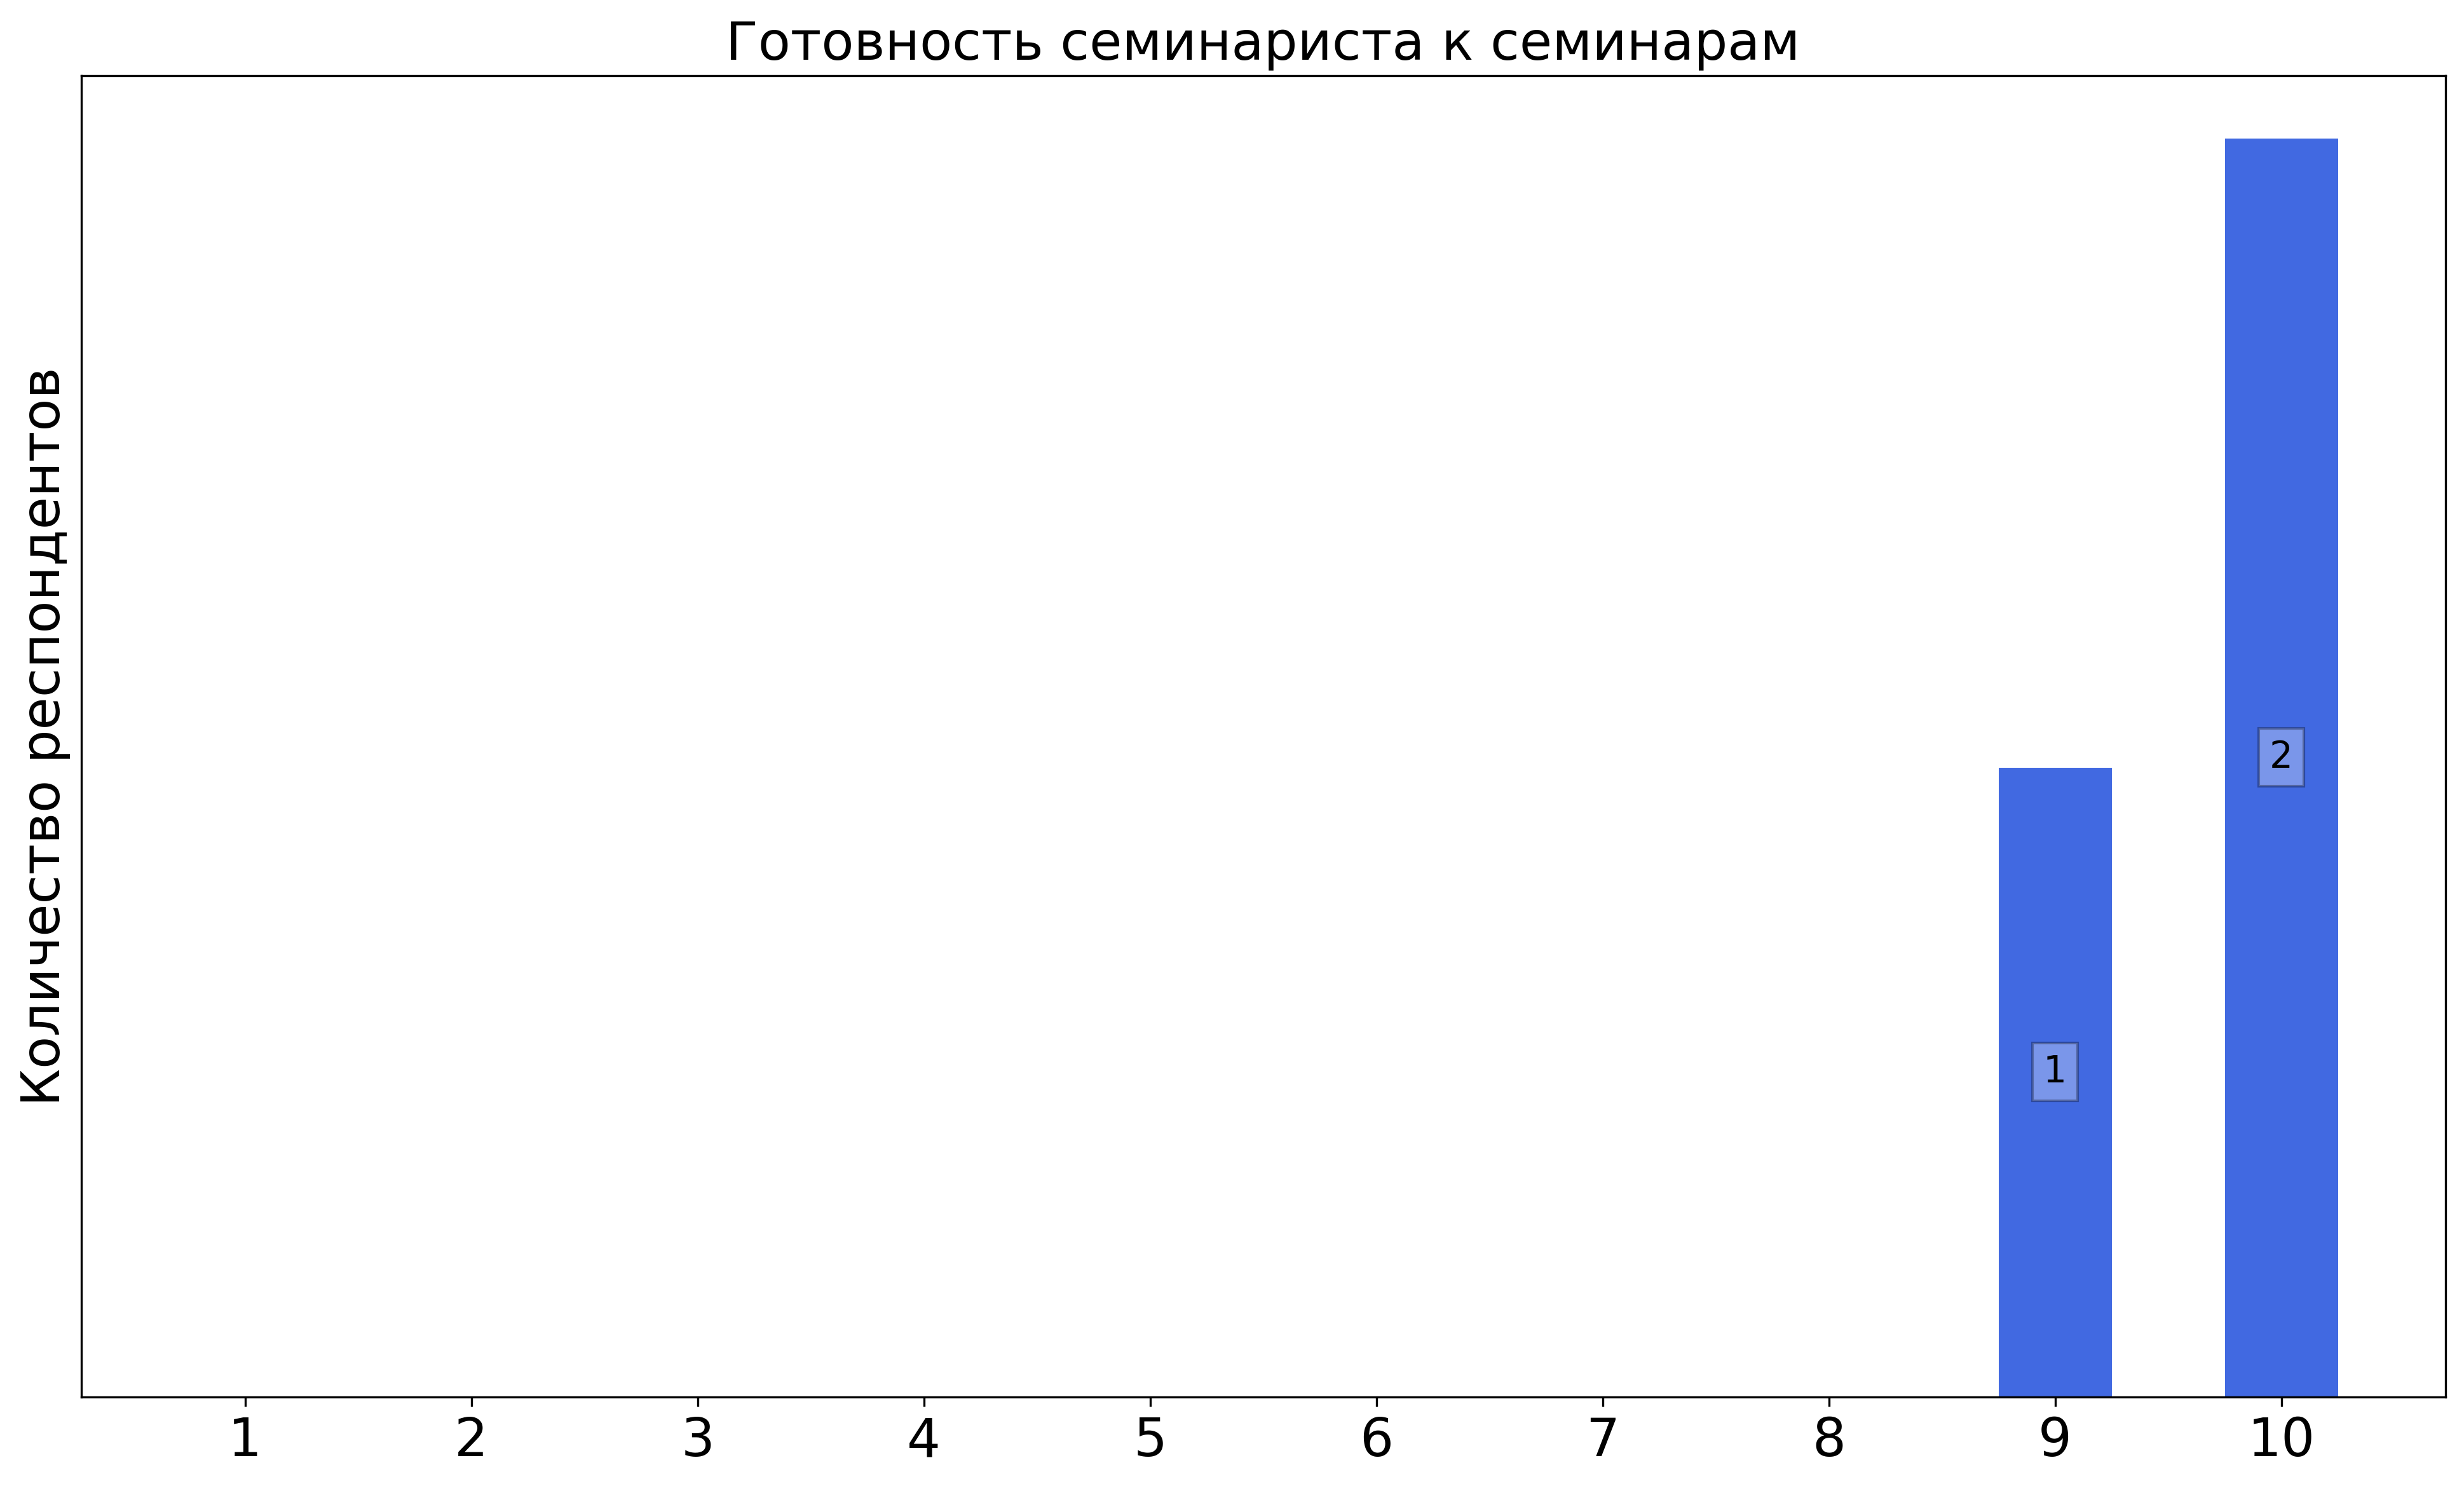
\includegraphics[width=\textwidth]{images/2 course/Дифференциальные уравнения/seminarists-marks-Глухова Е.В.-1.png}
			\end{subfigure}
			\begin{subfigure}[b]{0.45\textwidth}
				\centering
				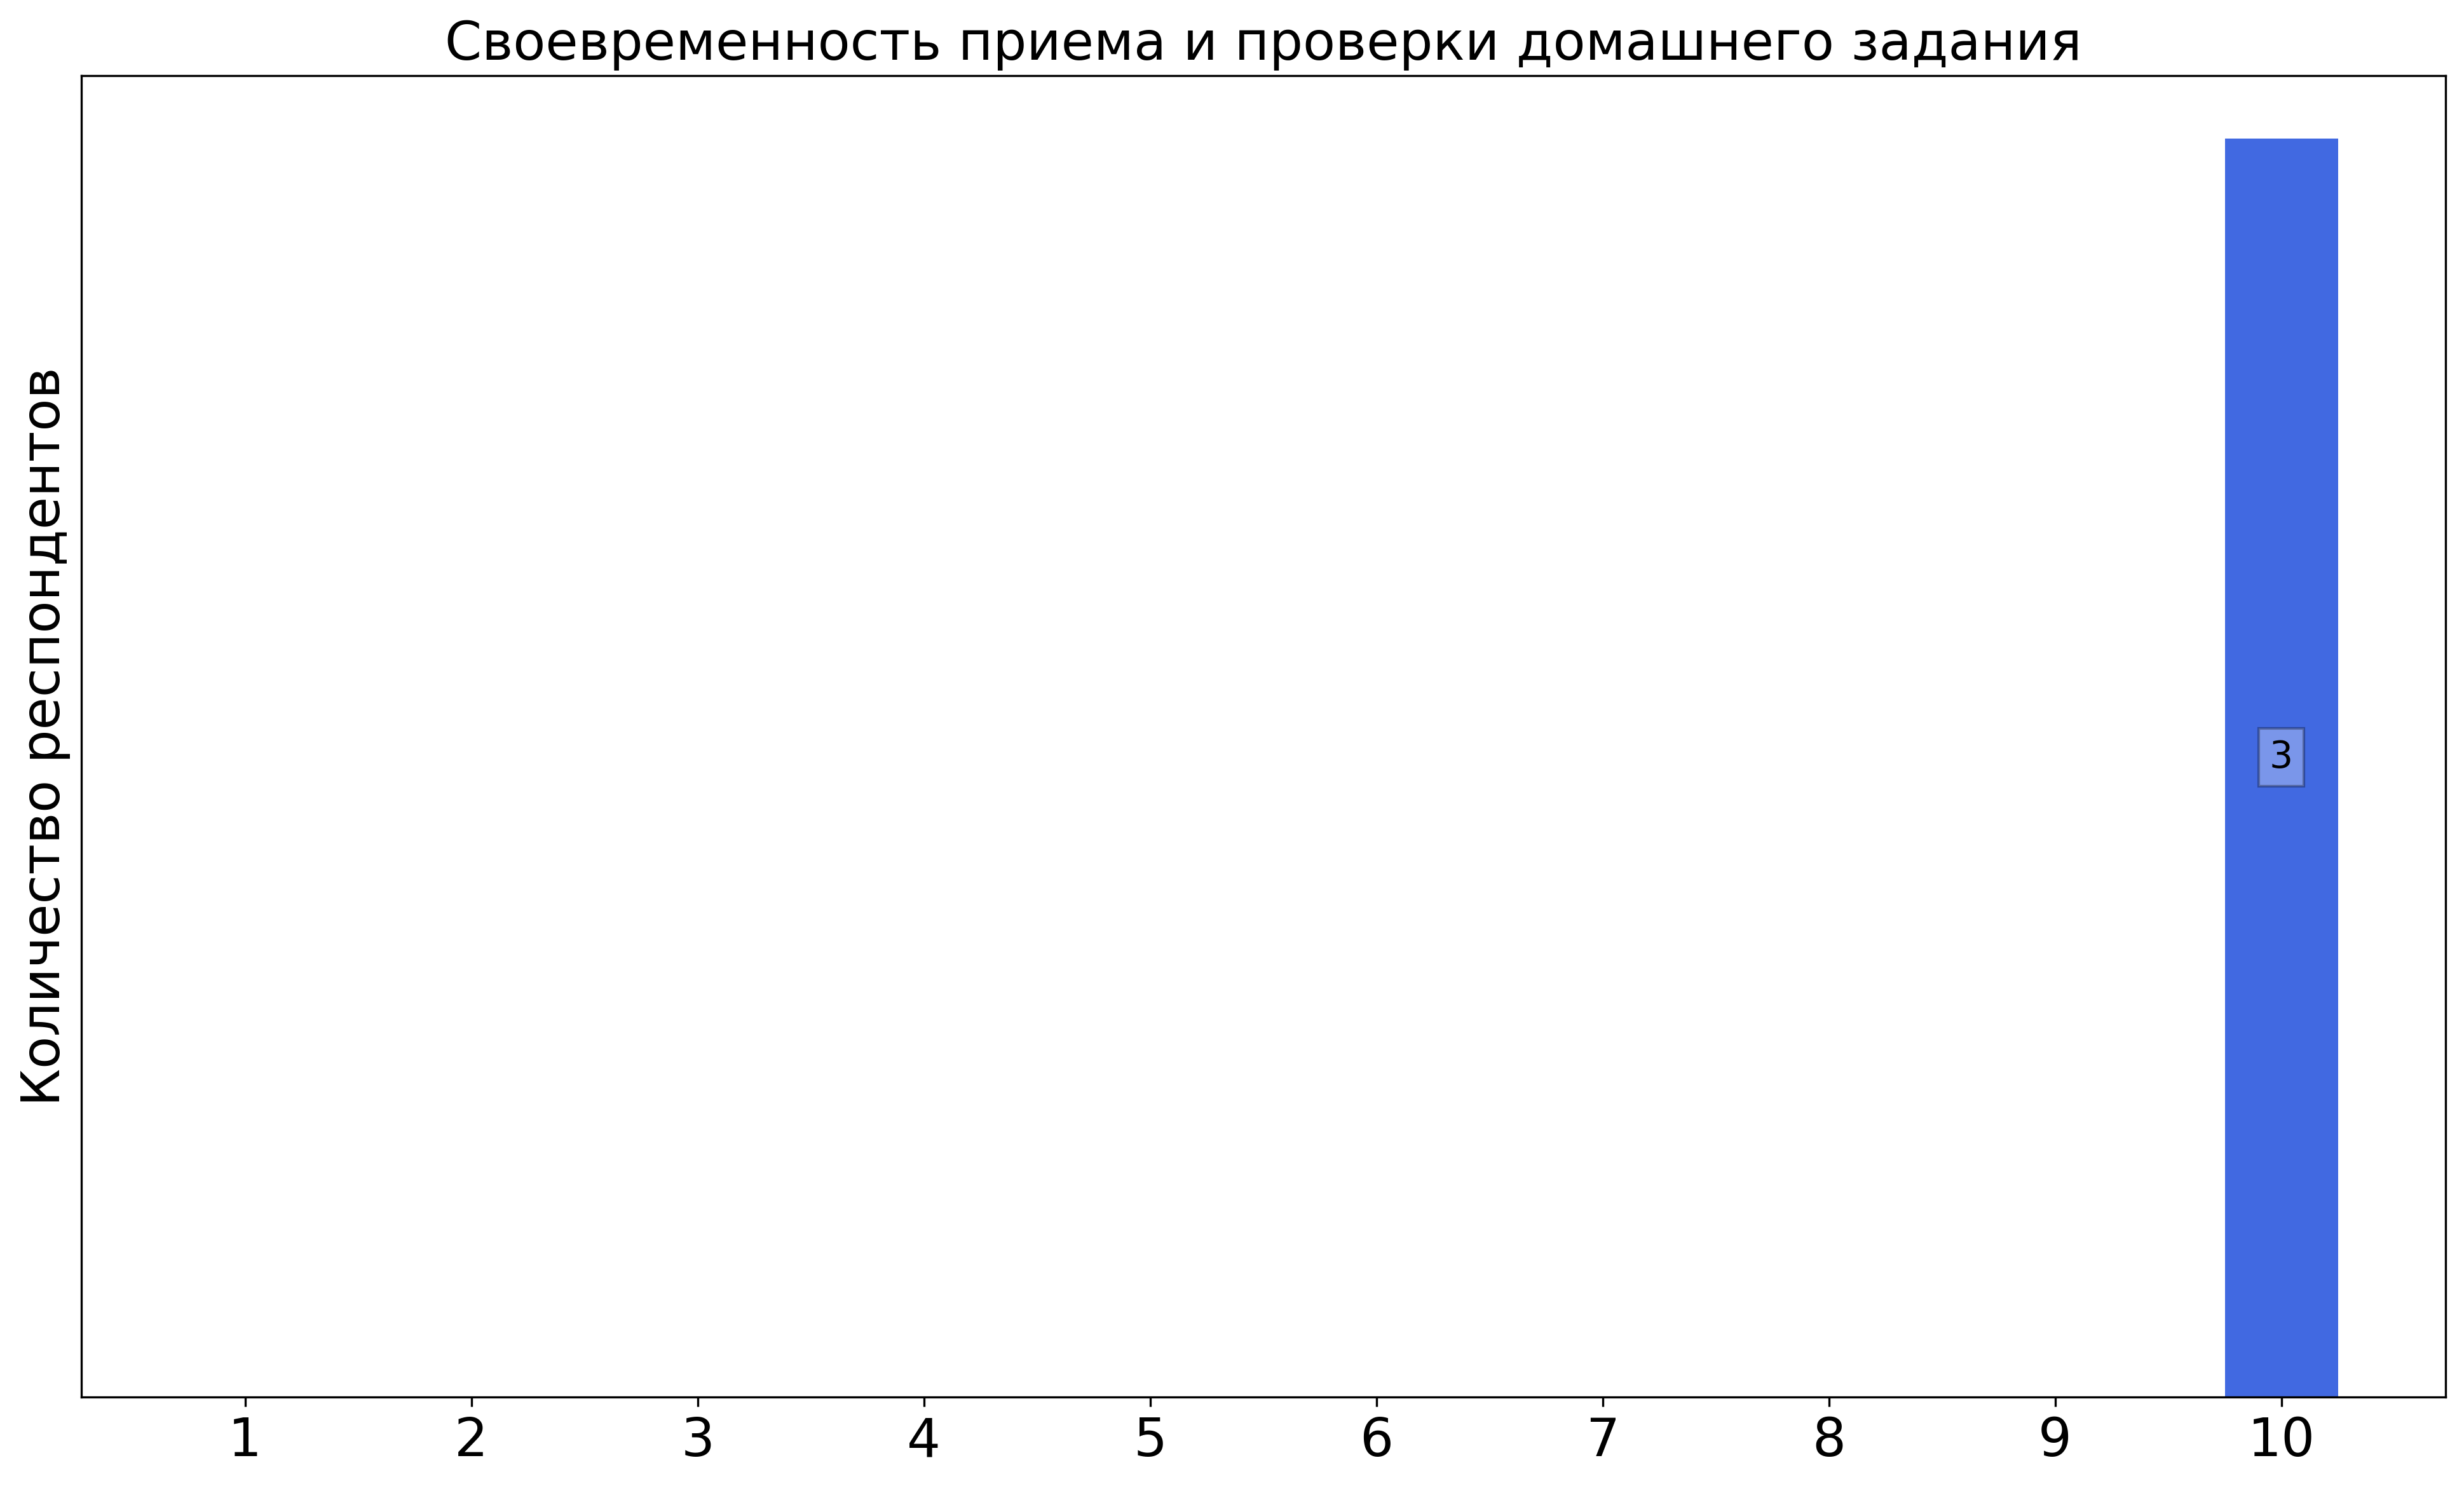
\includegraphics[width=\textwidth]{images/2 course/Дифференциальные уравнения/seminarists-marks-Глухова Е.В.-2.png}
			\end{subfigure}
			\begin{subfigure}[b]{0.45\textwidth}
				\centering
				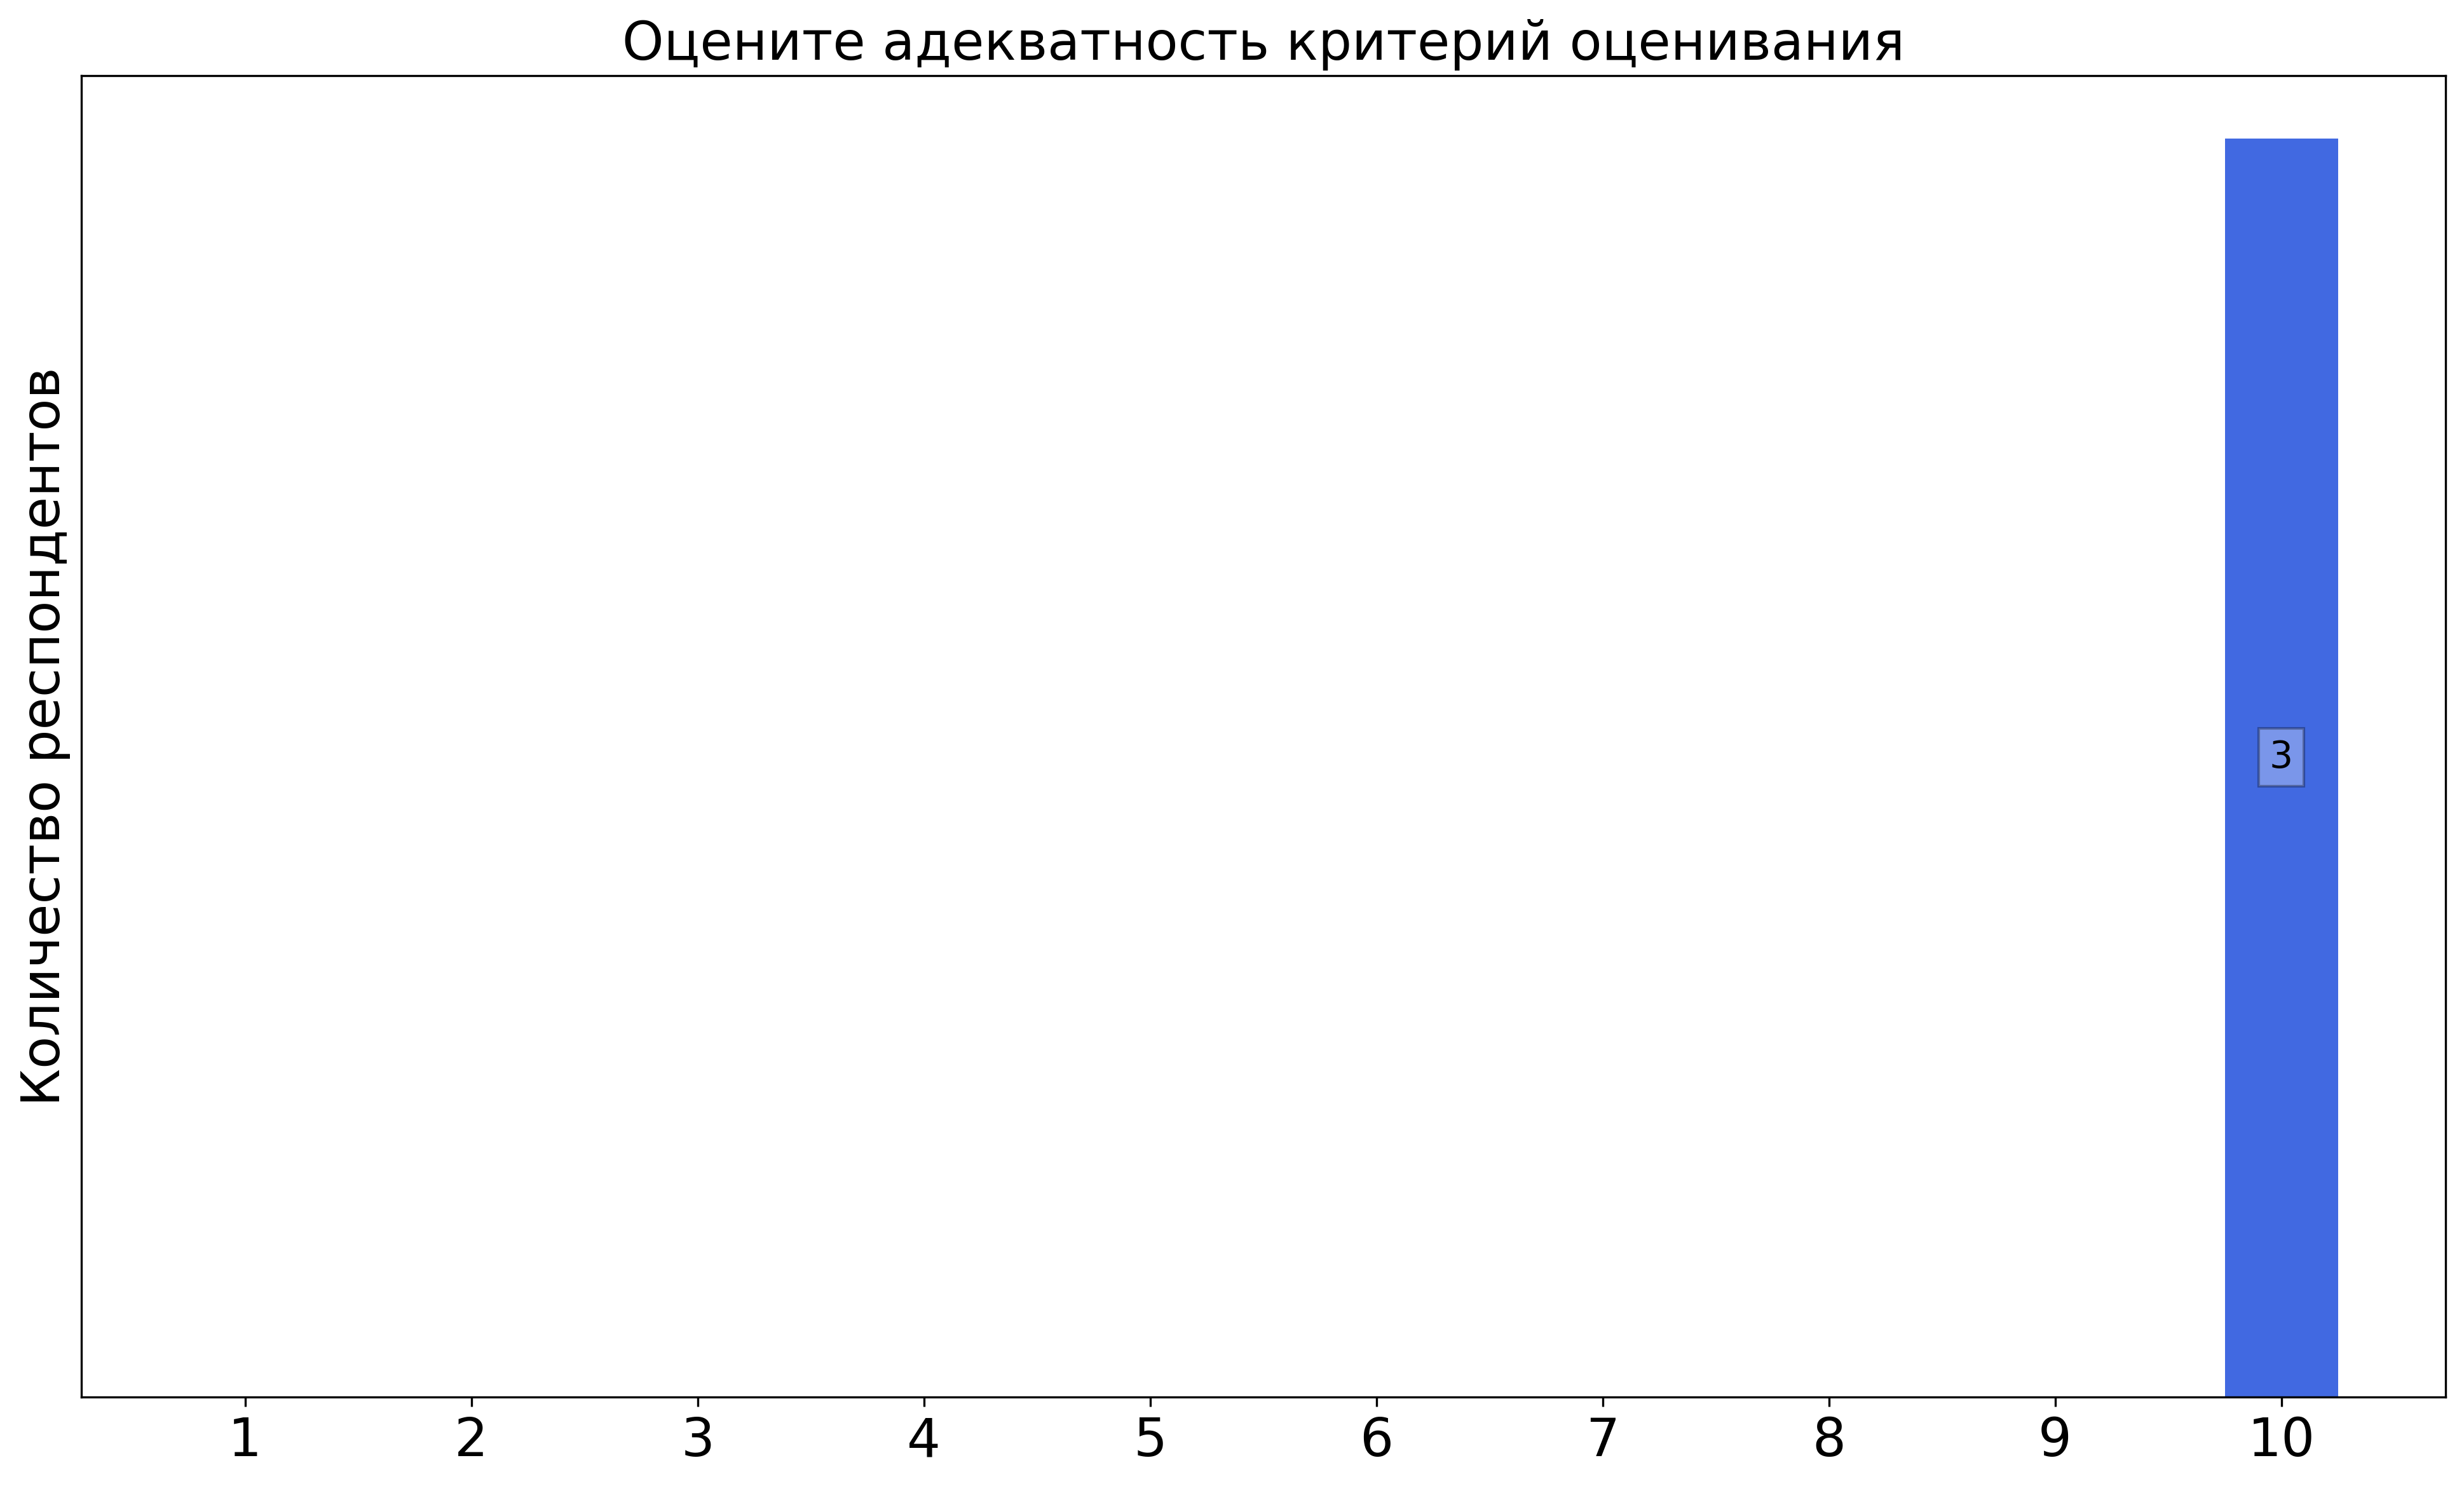
\includegraphics[width=\textwidth]{images/2 course/Дифференциальные уравнения/seminarists-marks-Глухова Е.В.-3.png}
			\end{subfigure}	
			\caption{Оценки респондентов о качестве преподавания семинаров}
		\end{figure}

            
    \subsubsection{Отзыв студентов о семинарах. Семинарист: Петрович А.Ю.}
		\begin{figure}[H]
			\centering
			\begin{subfigure}[b]{0.45\textwidth}
				\centering
				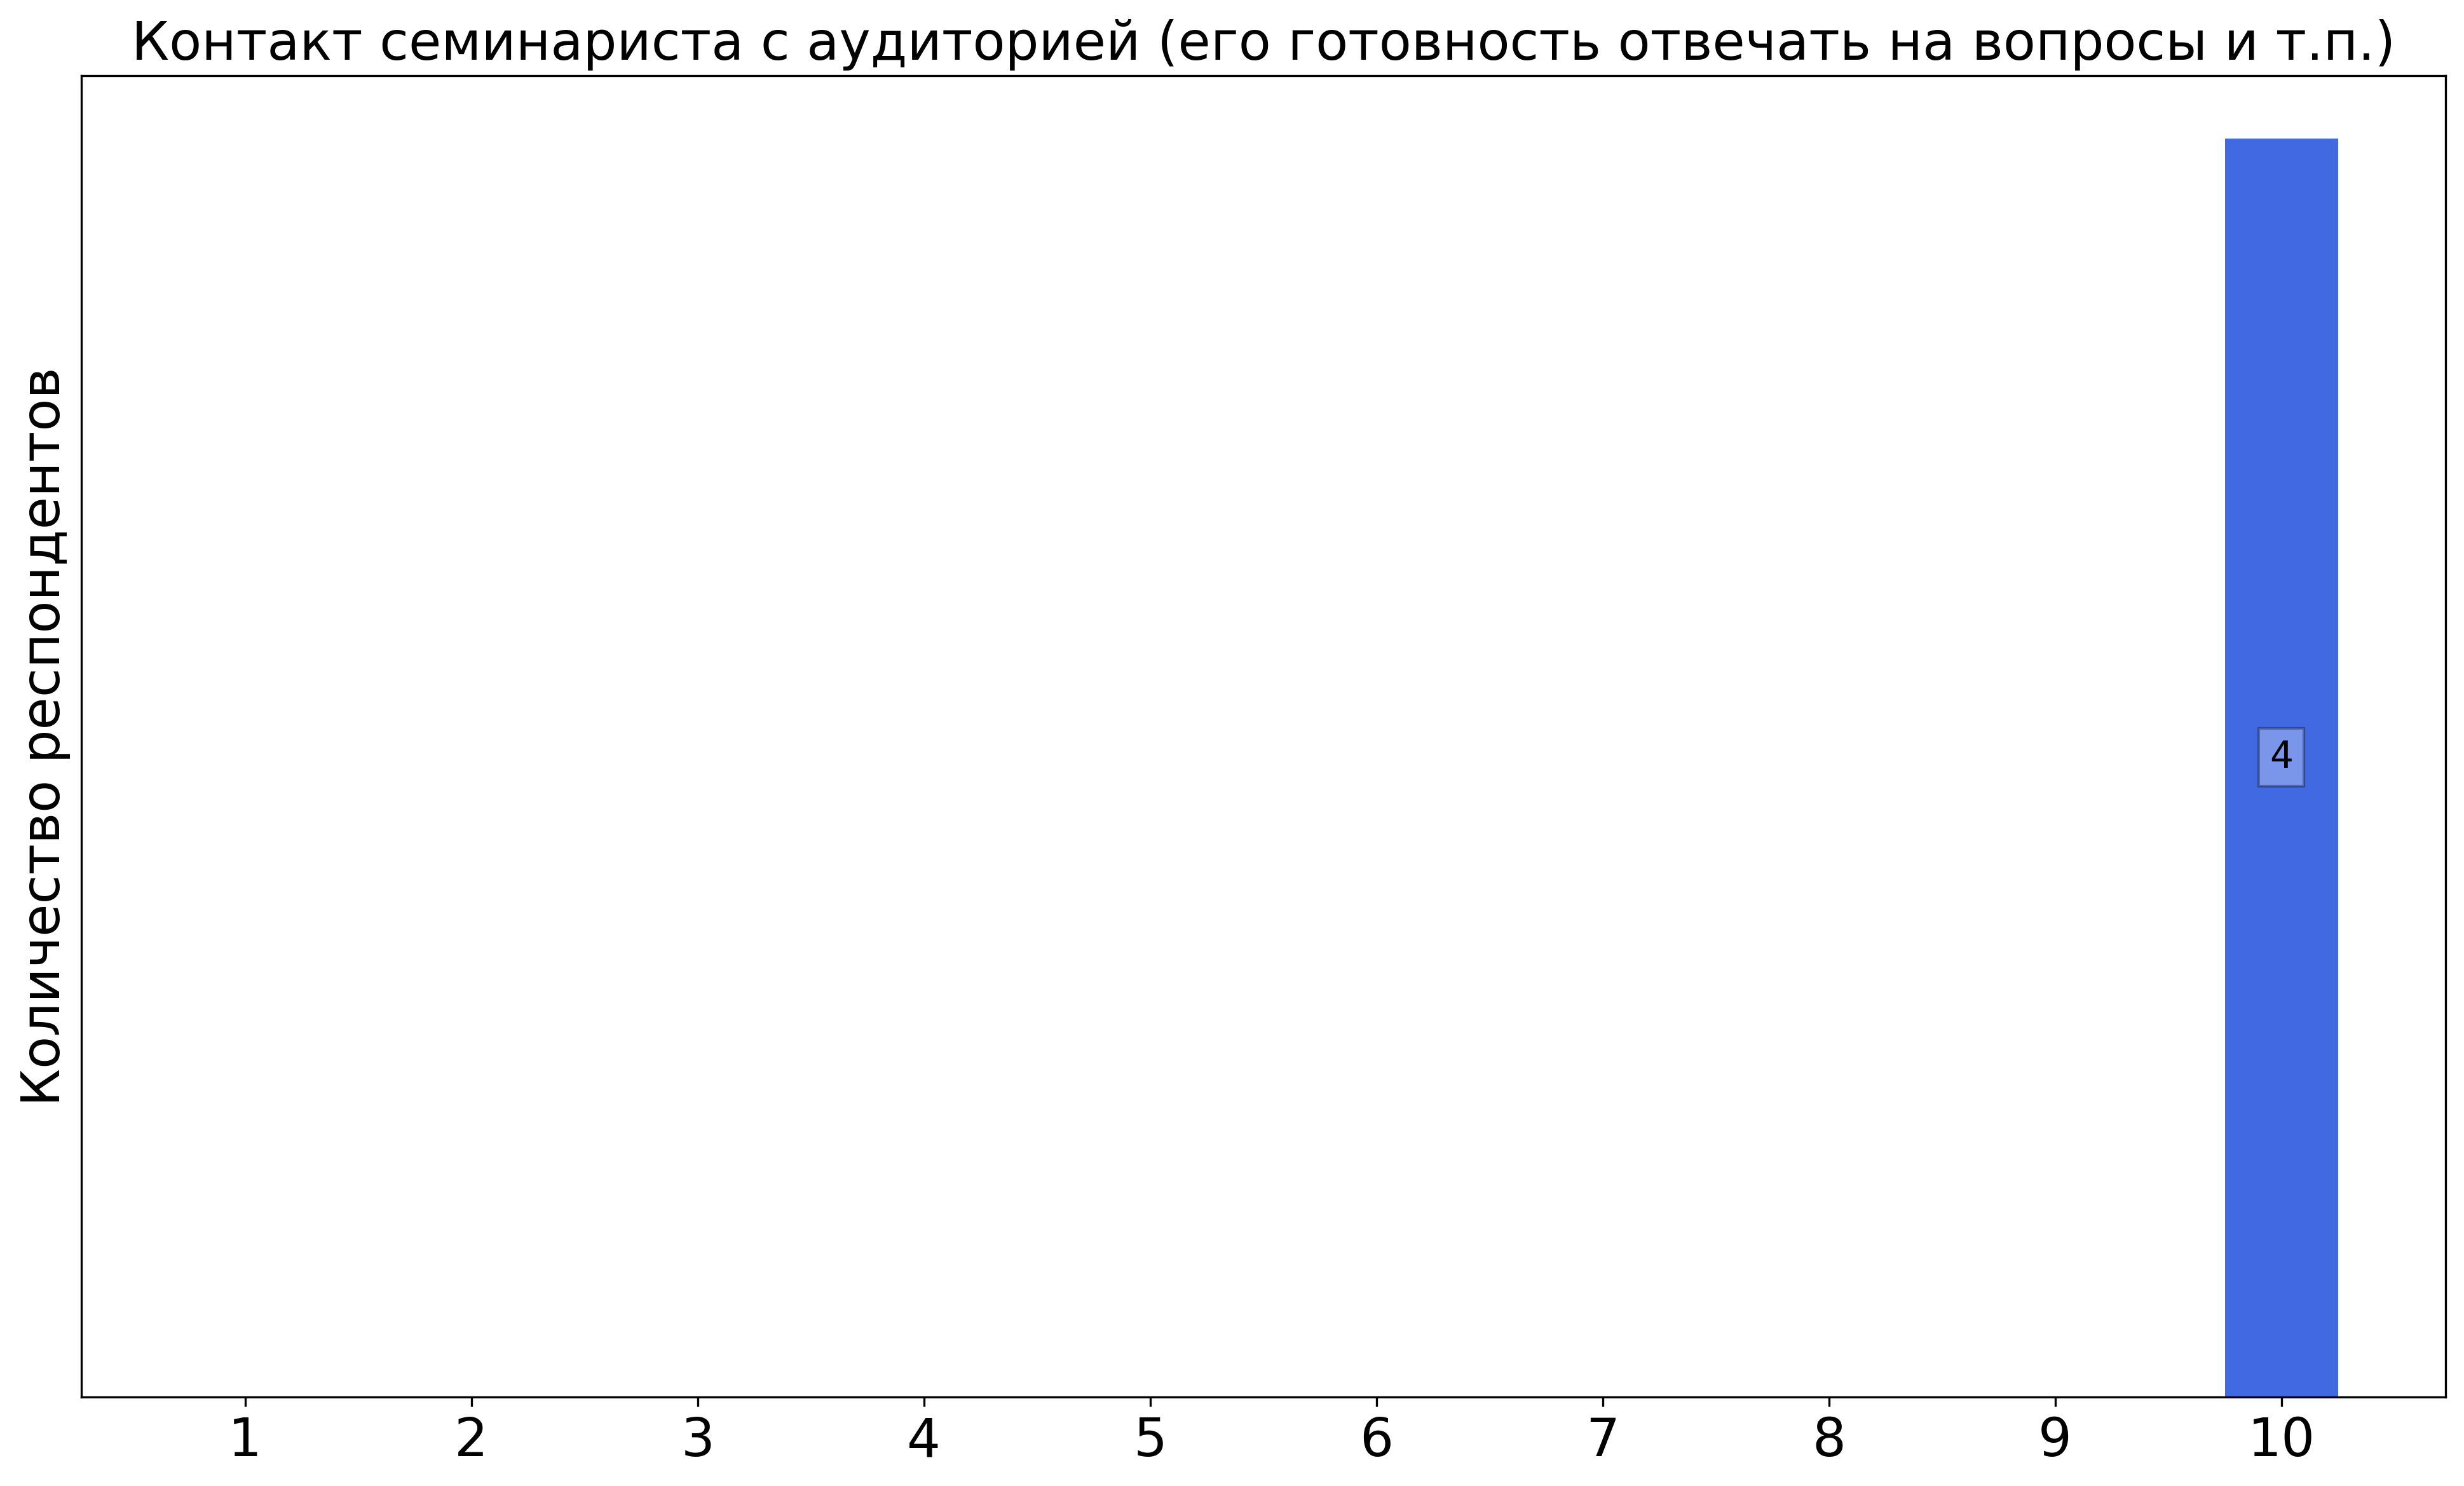
\includegraphics[width=\textwidth]{images/2 course/Дифференциальные уравнения/seminarists-marks-Петрович А.Ю.-0.png}
			\end{subfigure}
			\begin{subfigure}[b]{0.45\textwidth}
				\centering
				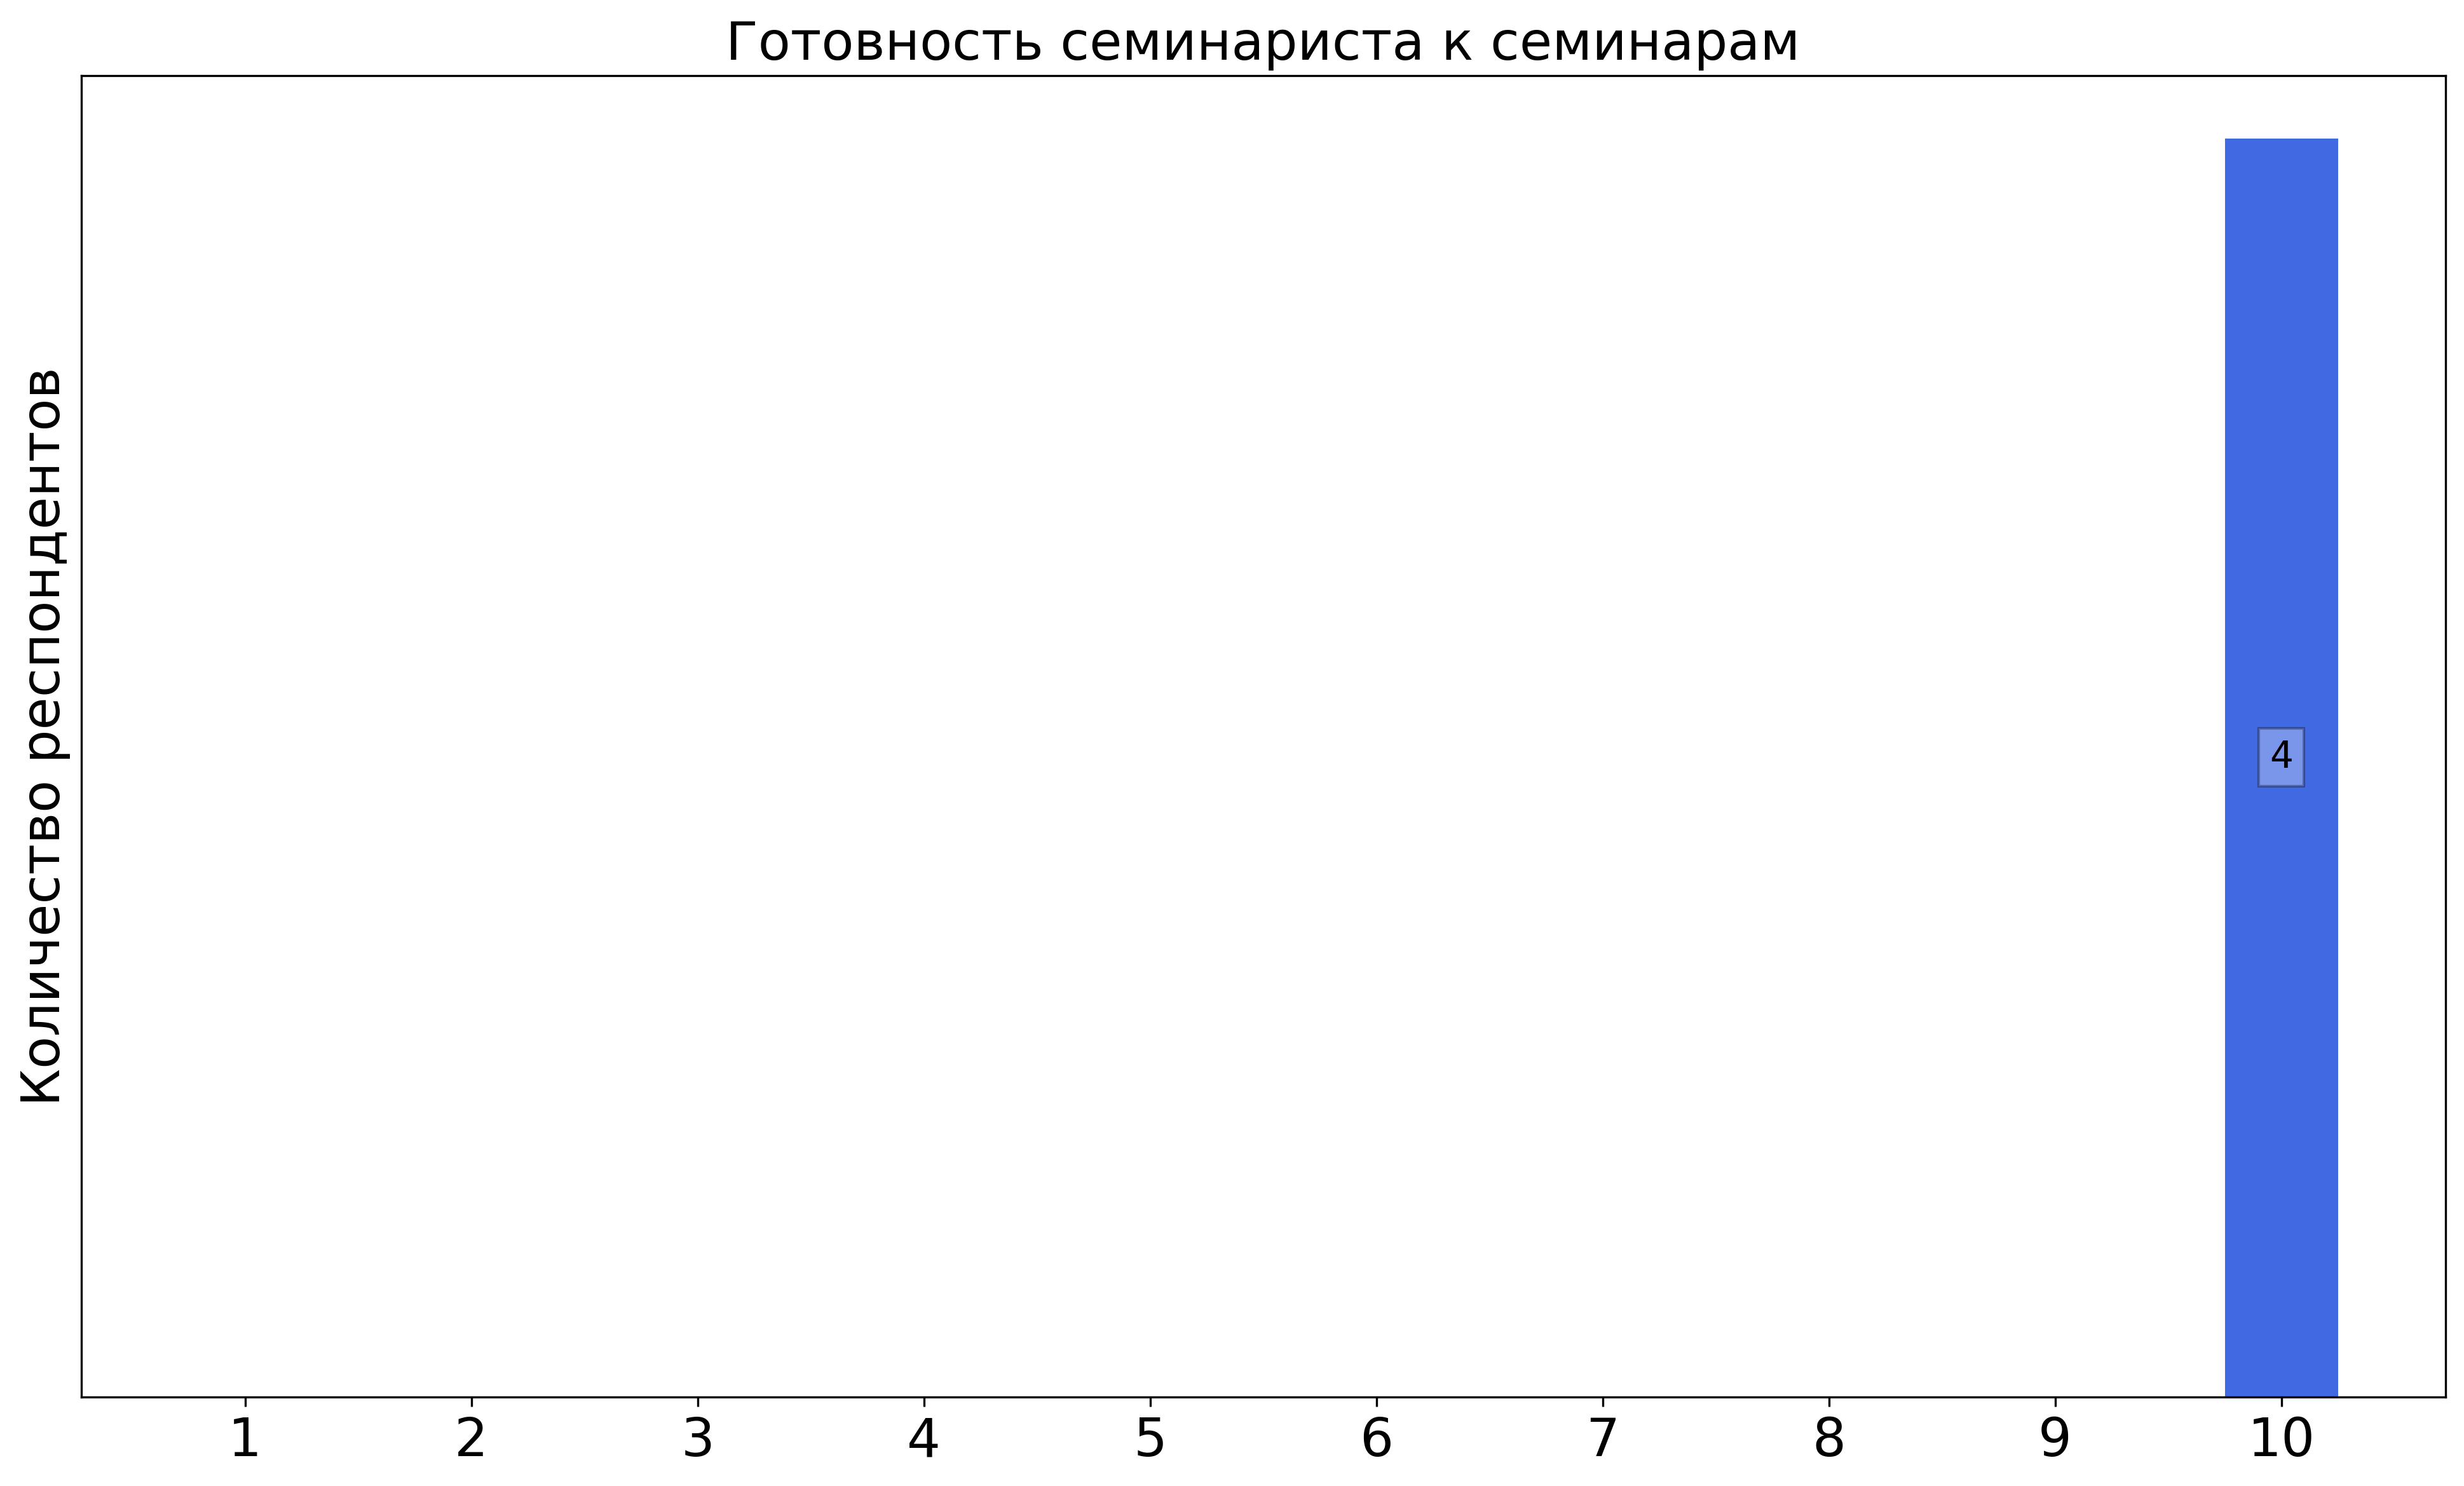
\includegraphics[width=\textwidth]{images/2 course/Дифференциальные уравнения/seminarists-marks-Петрович А.Ю.-1.png}
			\end{subfigure}
			\begin{subfigure}[b]{0.45\textwidth}
				\centering
				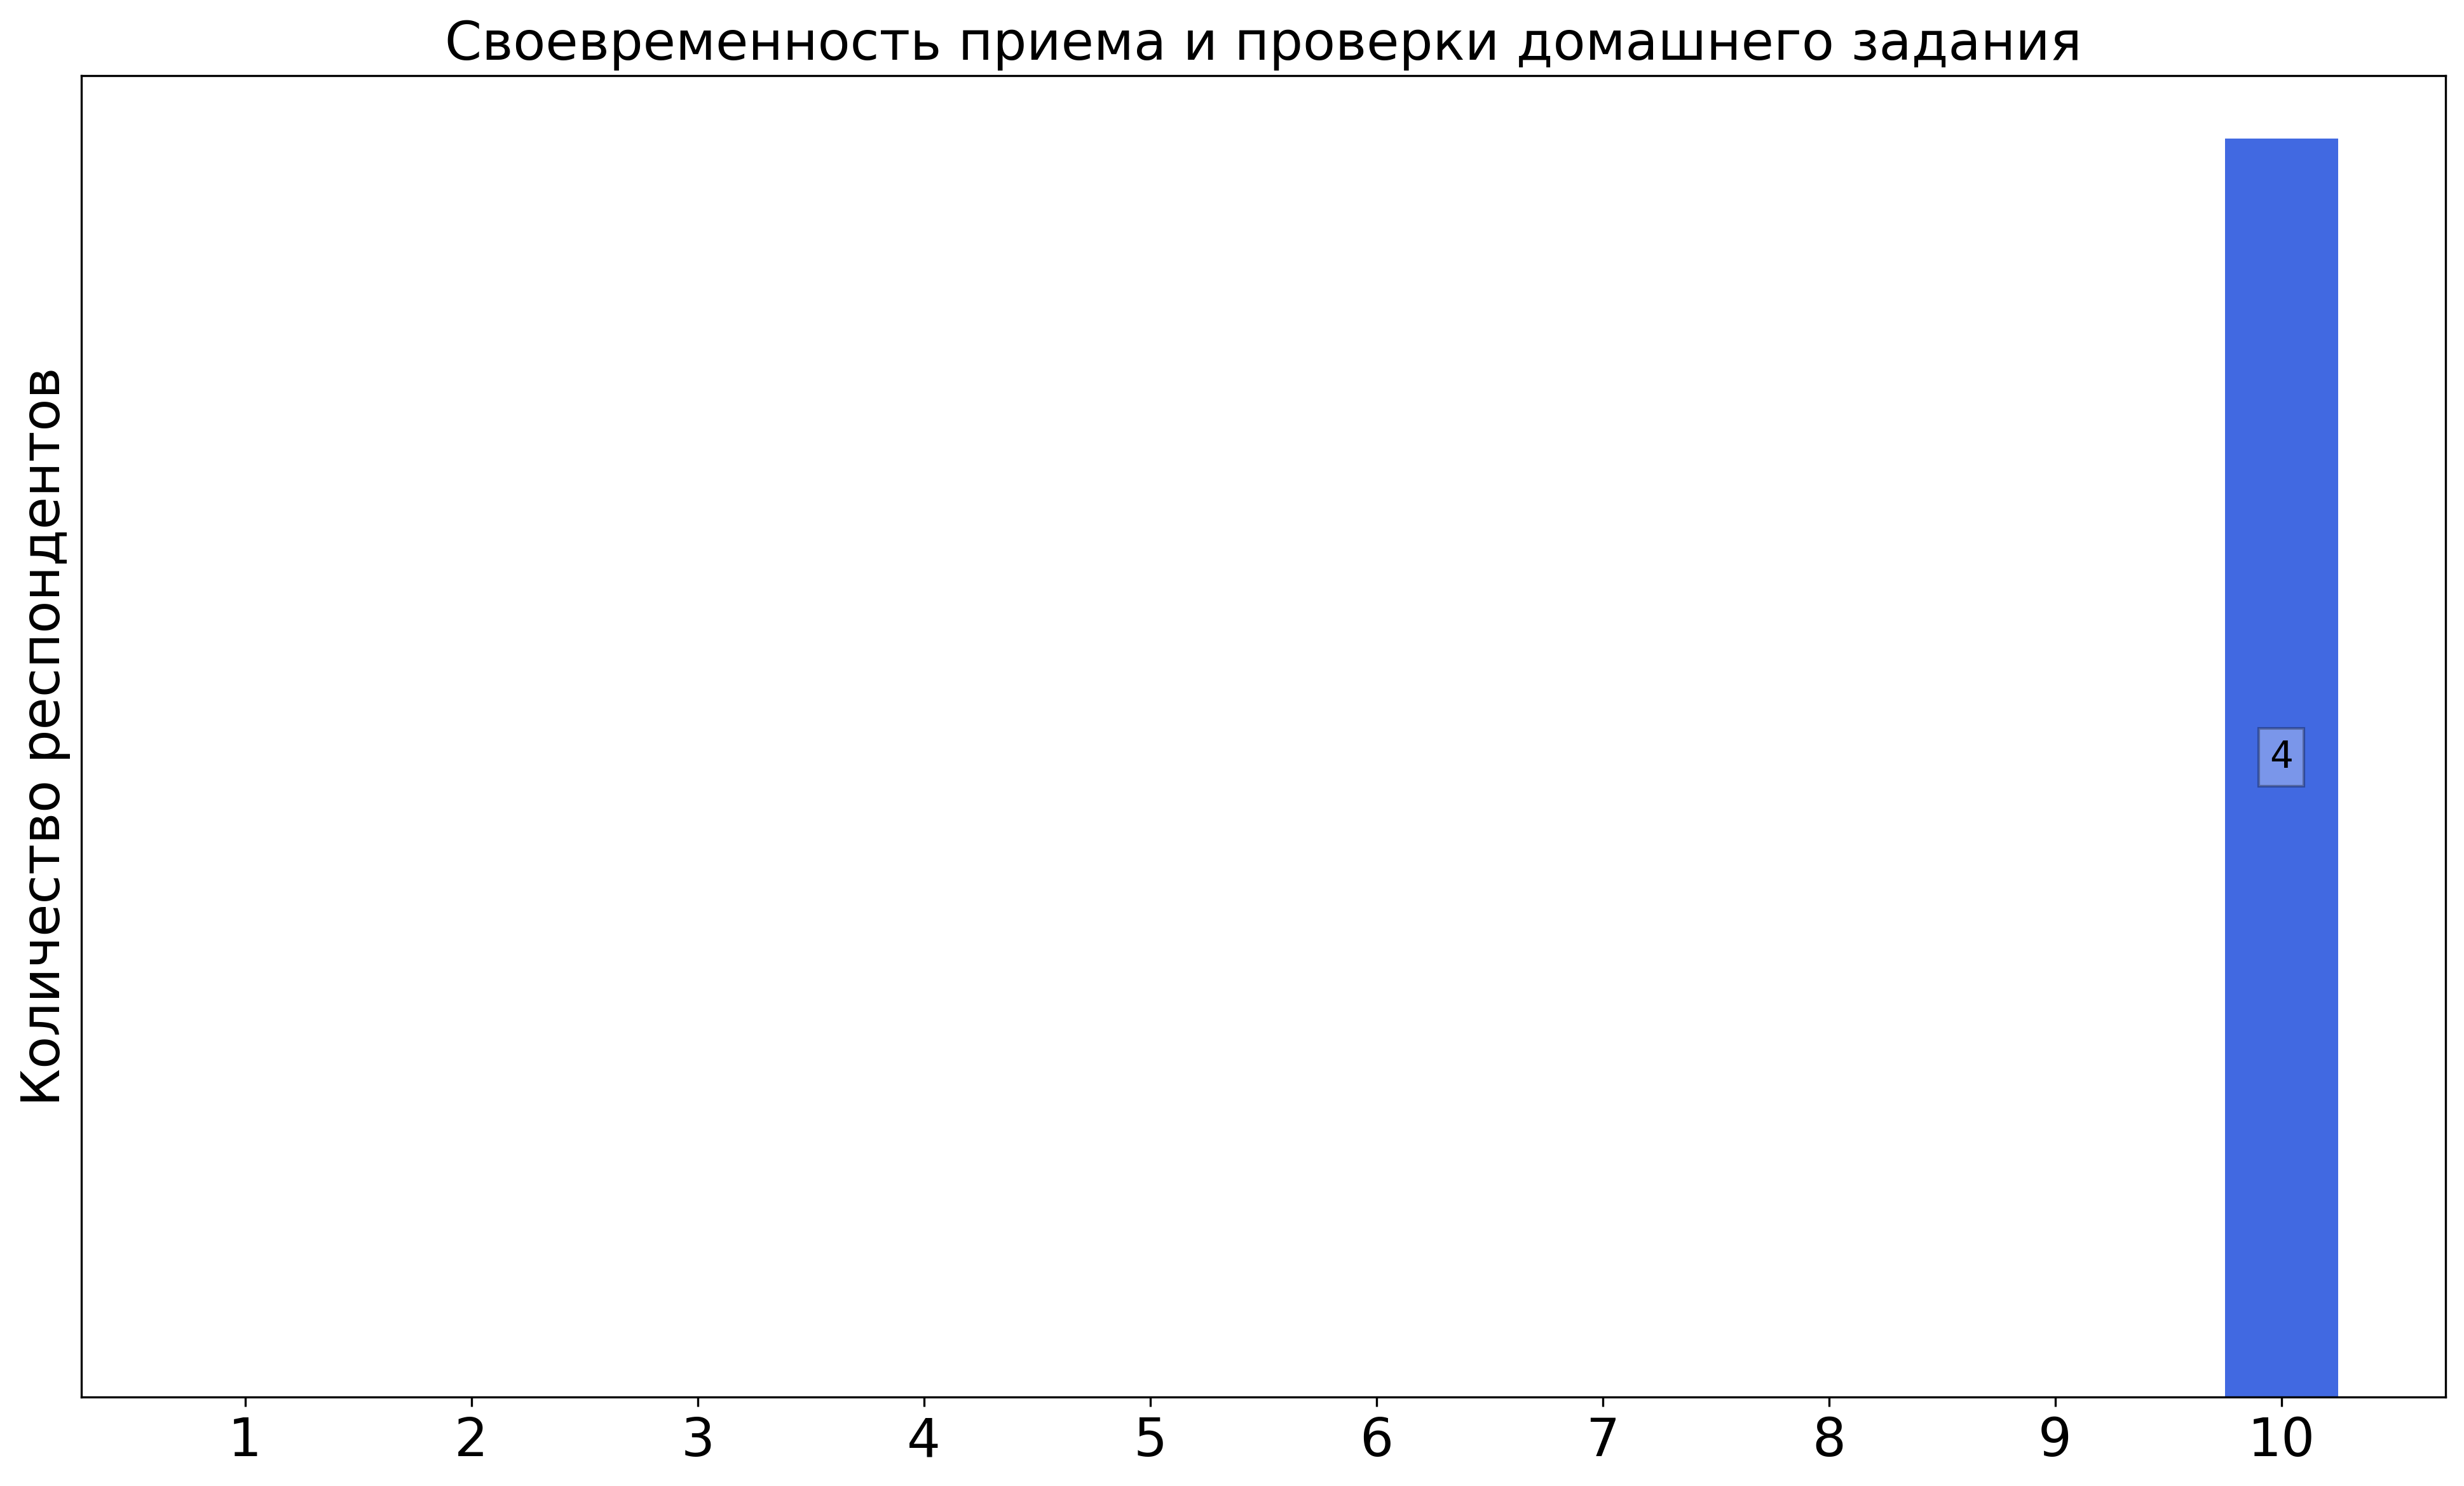
\includegraphics[width=\textwidth]{images/2 course/Дифференциальные уравнения/seminarists-marks-Петрович А.Ю.-2.png}
			\end{subfigure}
			\begin{subfigure}[b]{0.45\textwidth}
				\centering
				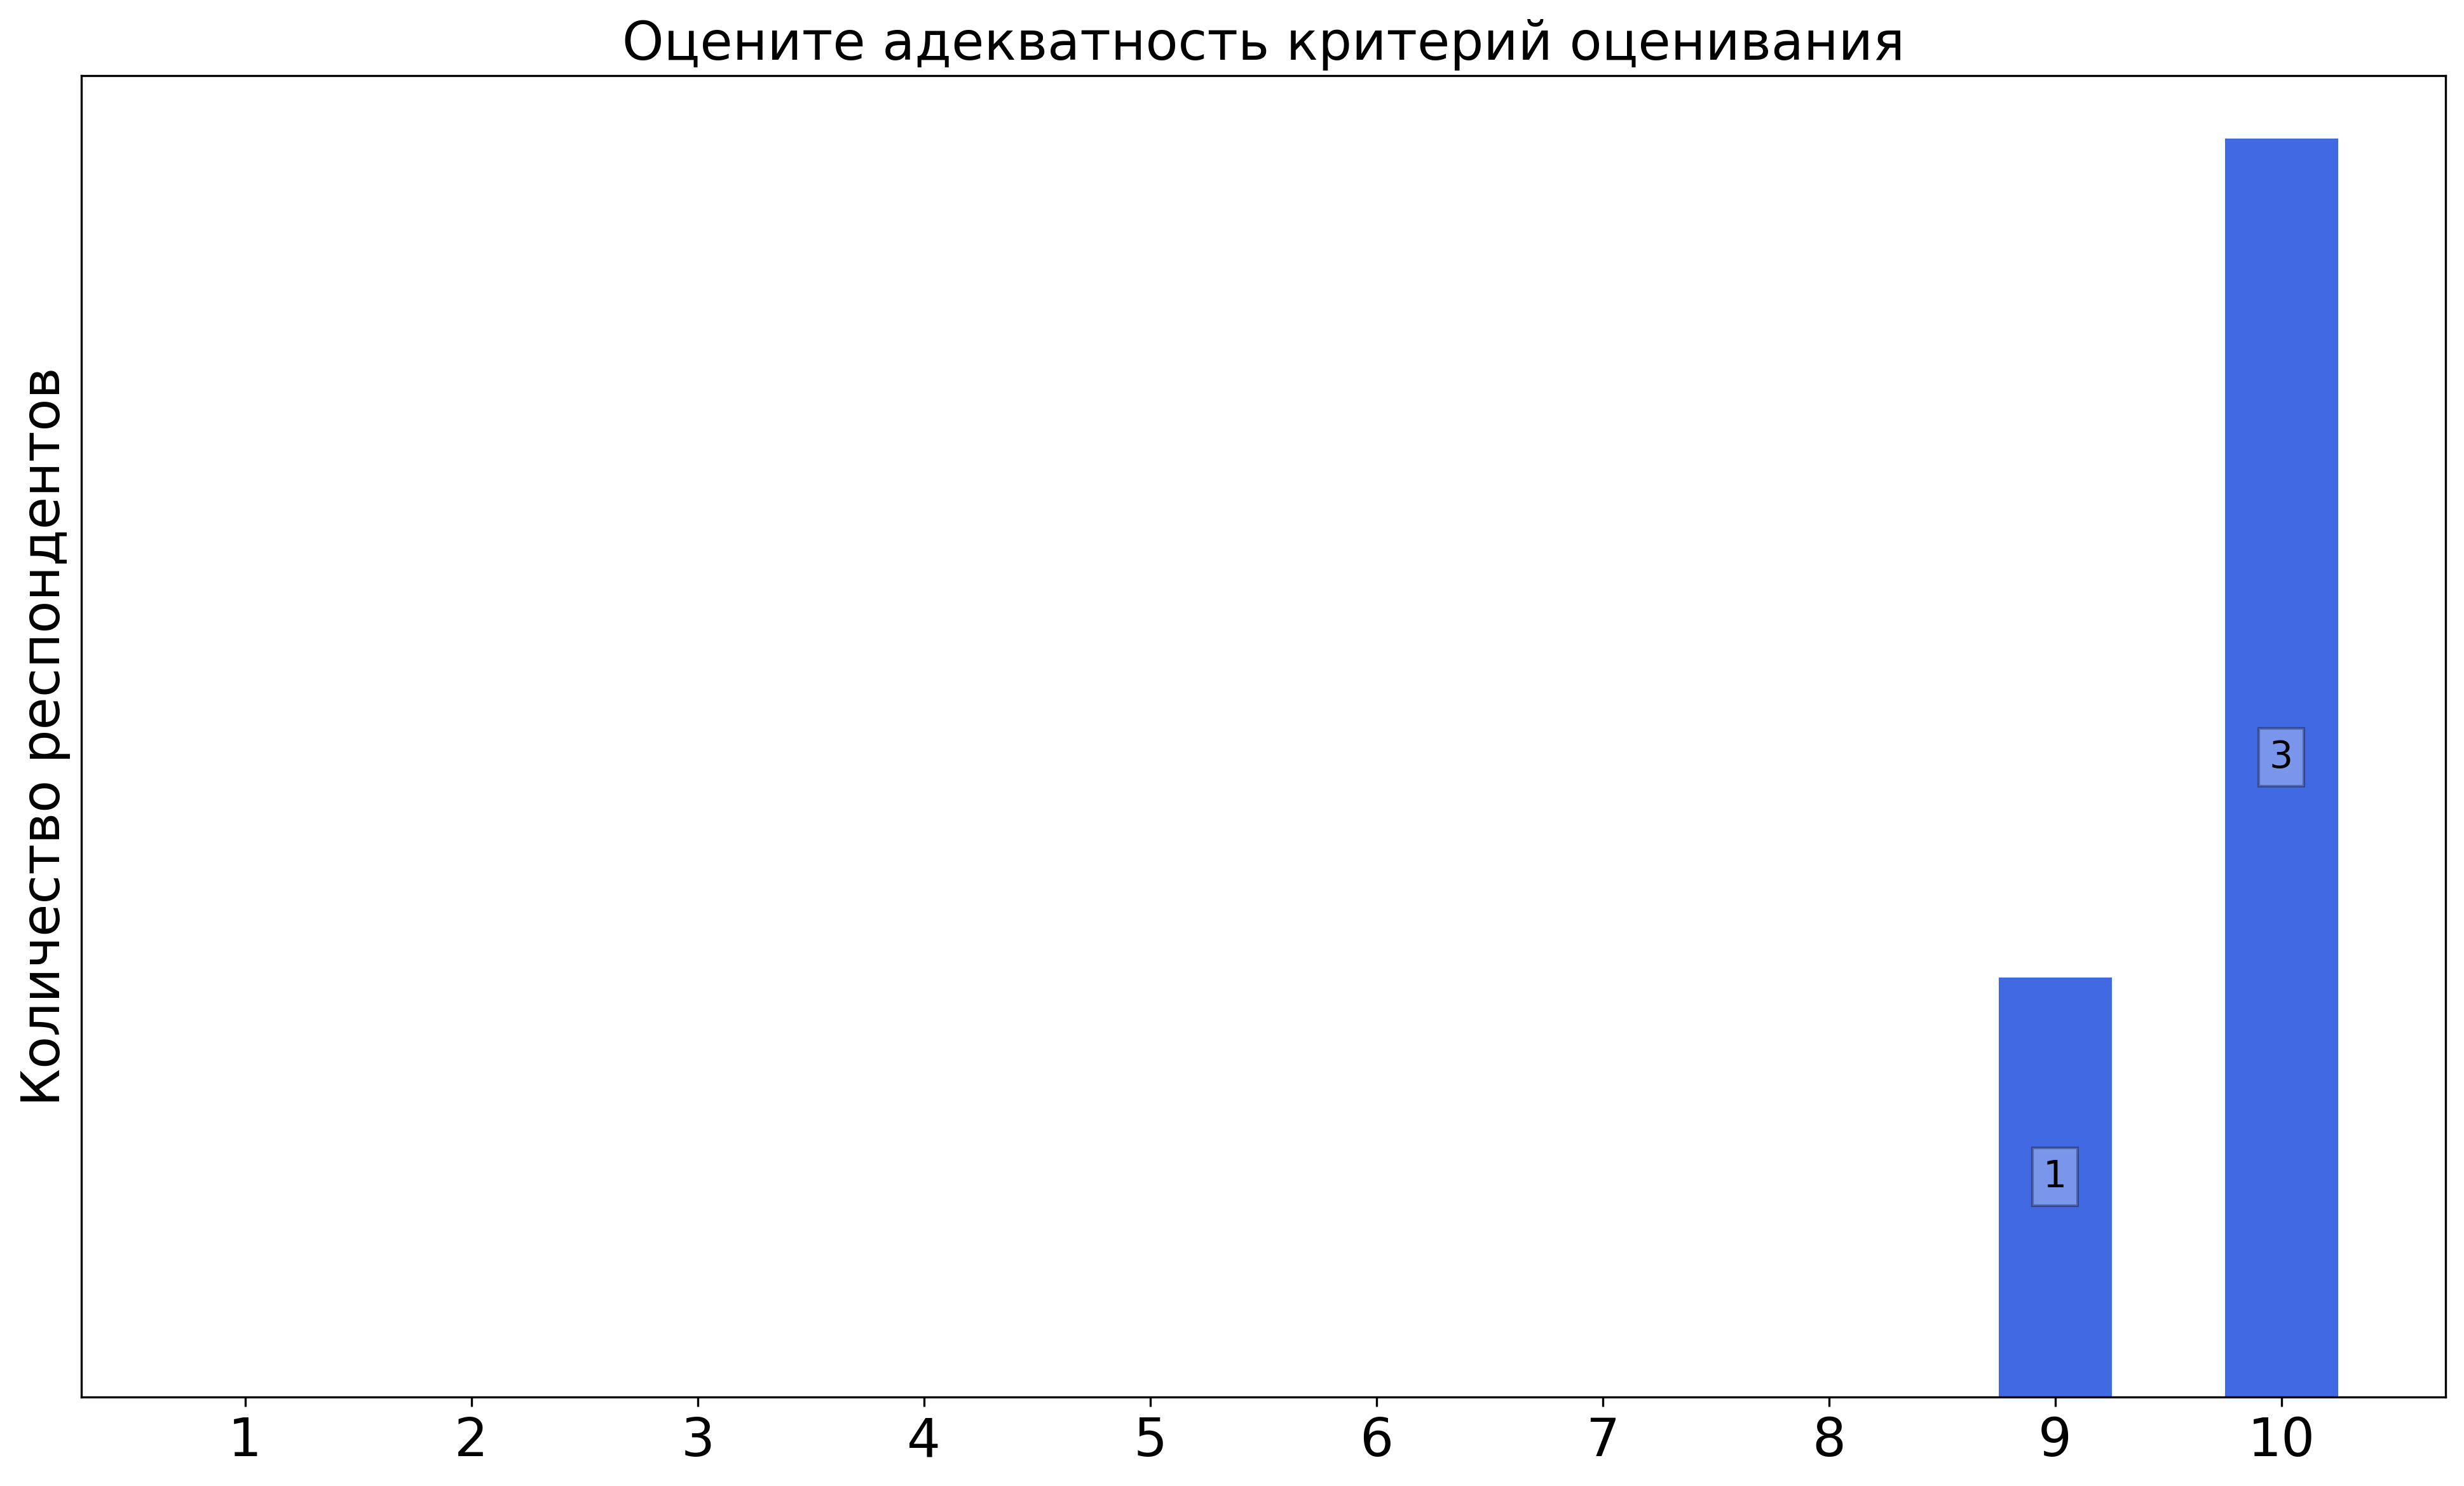
\includegraphics[width=\textwidth]{images/2 course/Дифференциальные уравнения/seminarists-marks-Петрович А.Ю.-3.png}
			\end{subfigure}	
			\caption{Оценки респондентов о качестве преподавания семинаров}
		\end{figure}

        
    \subsubsection{Отзыв студентов о семинарах. Семинарист: Родин М.М.}
        \begin{figure}[H]
            \centering
            \begin{subfigure}[b]{0.45\textwidth}
                \centering
                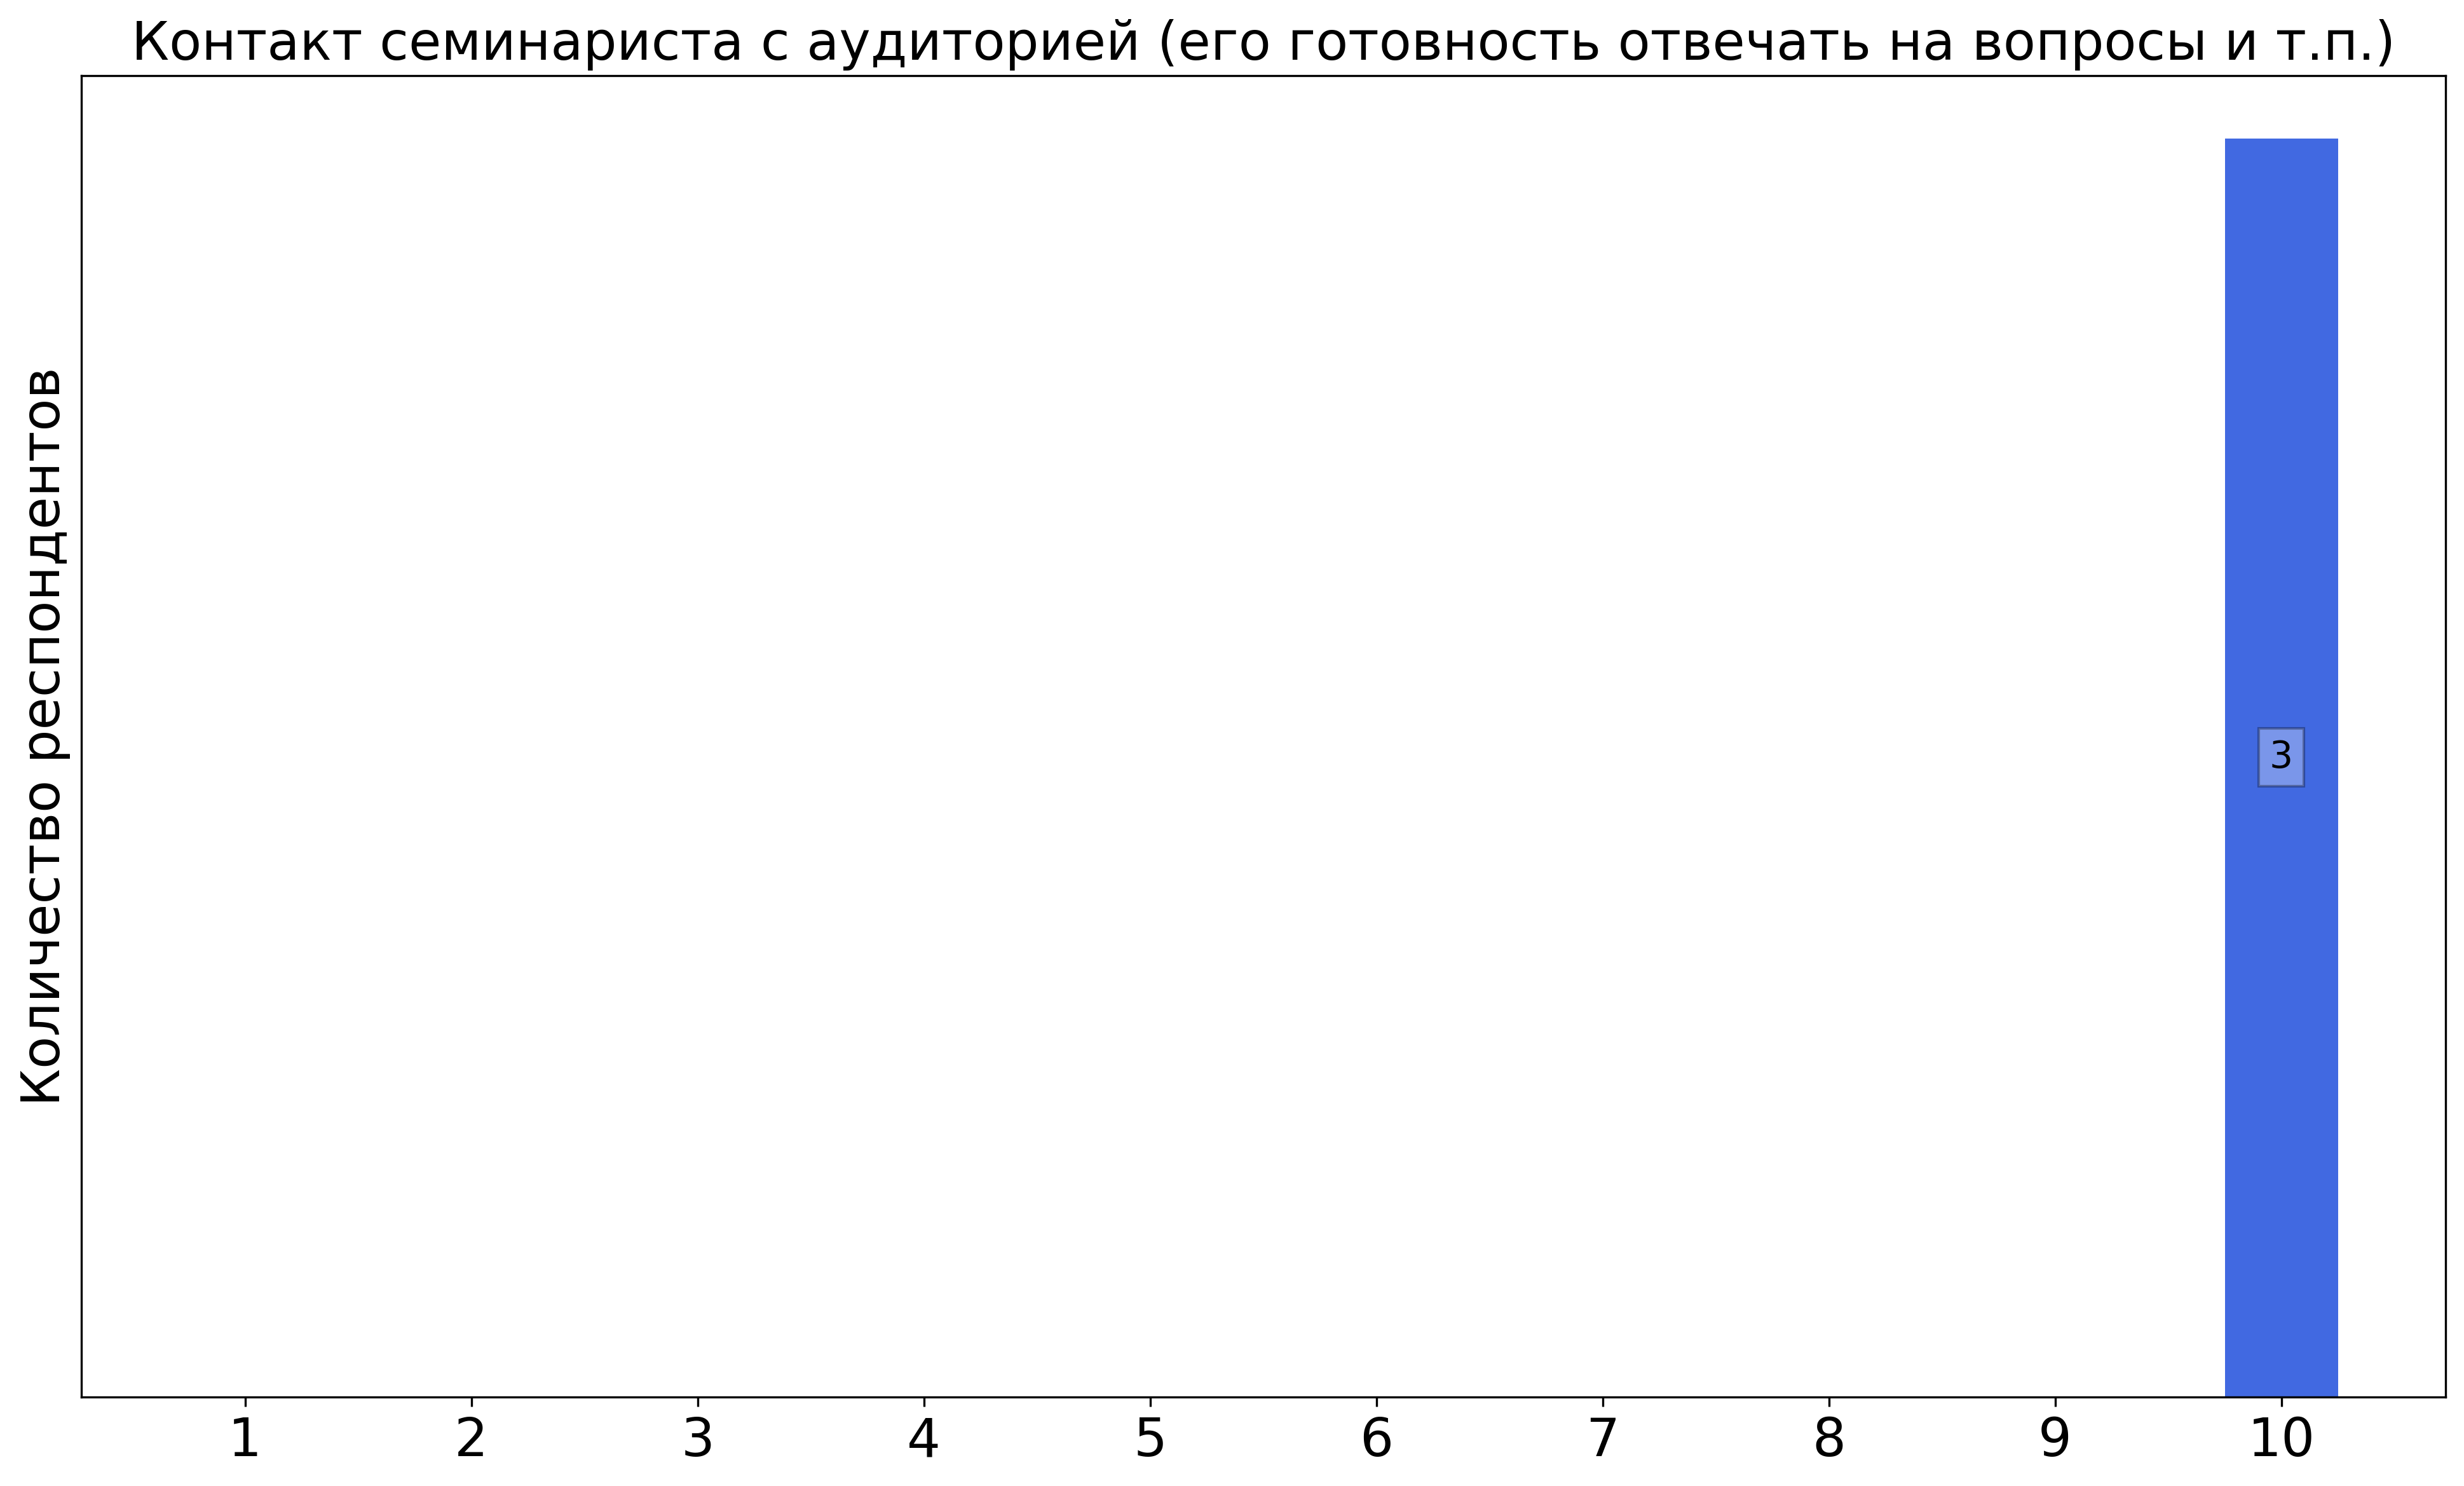
\includegraphics[width=\textwidth]{images/2 course/Дифференциальные уравнения/seminarists-marks-Родин М.М.-0.png}
            \end{subfigure}
            \begin{subfigure}[b]{0.45\textwidth}
                \centering
                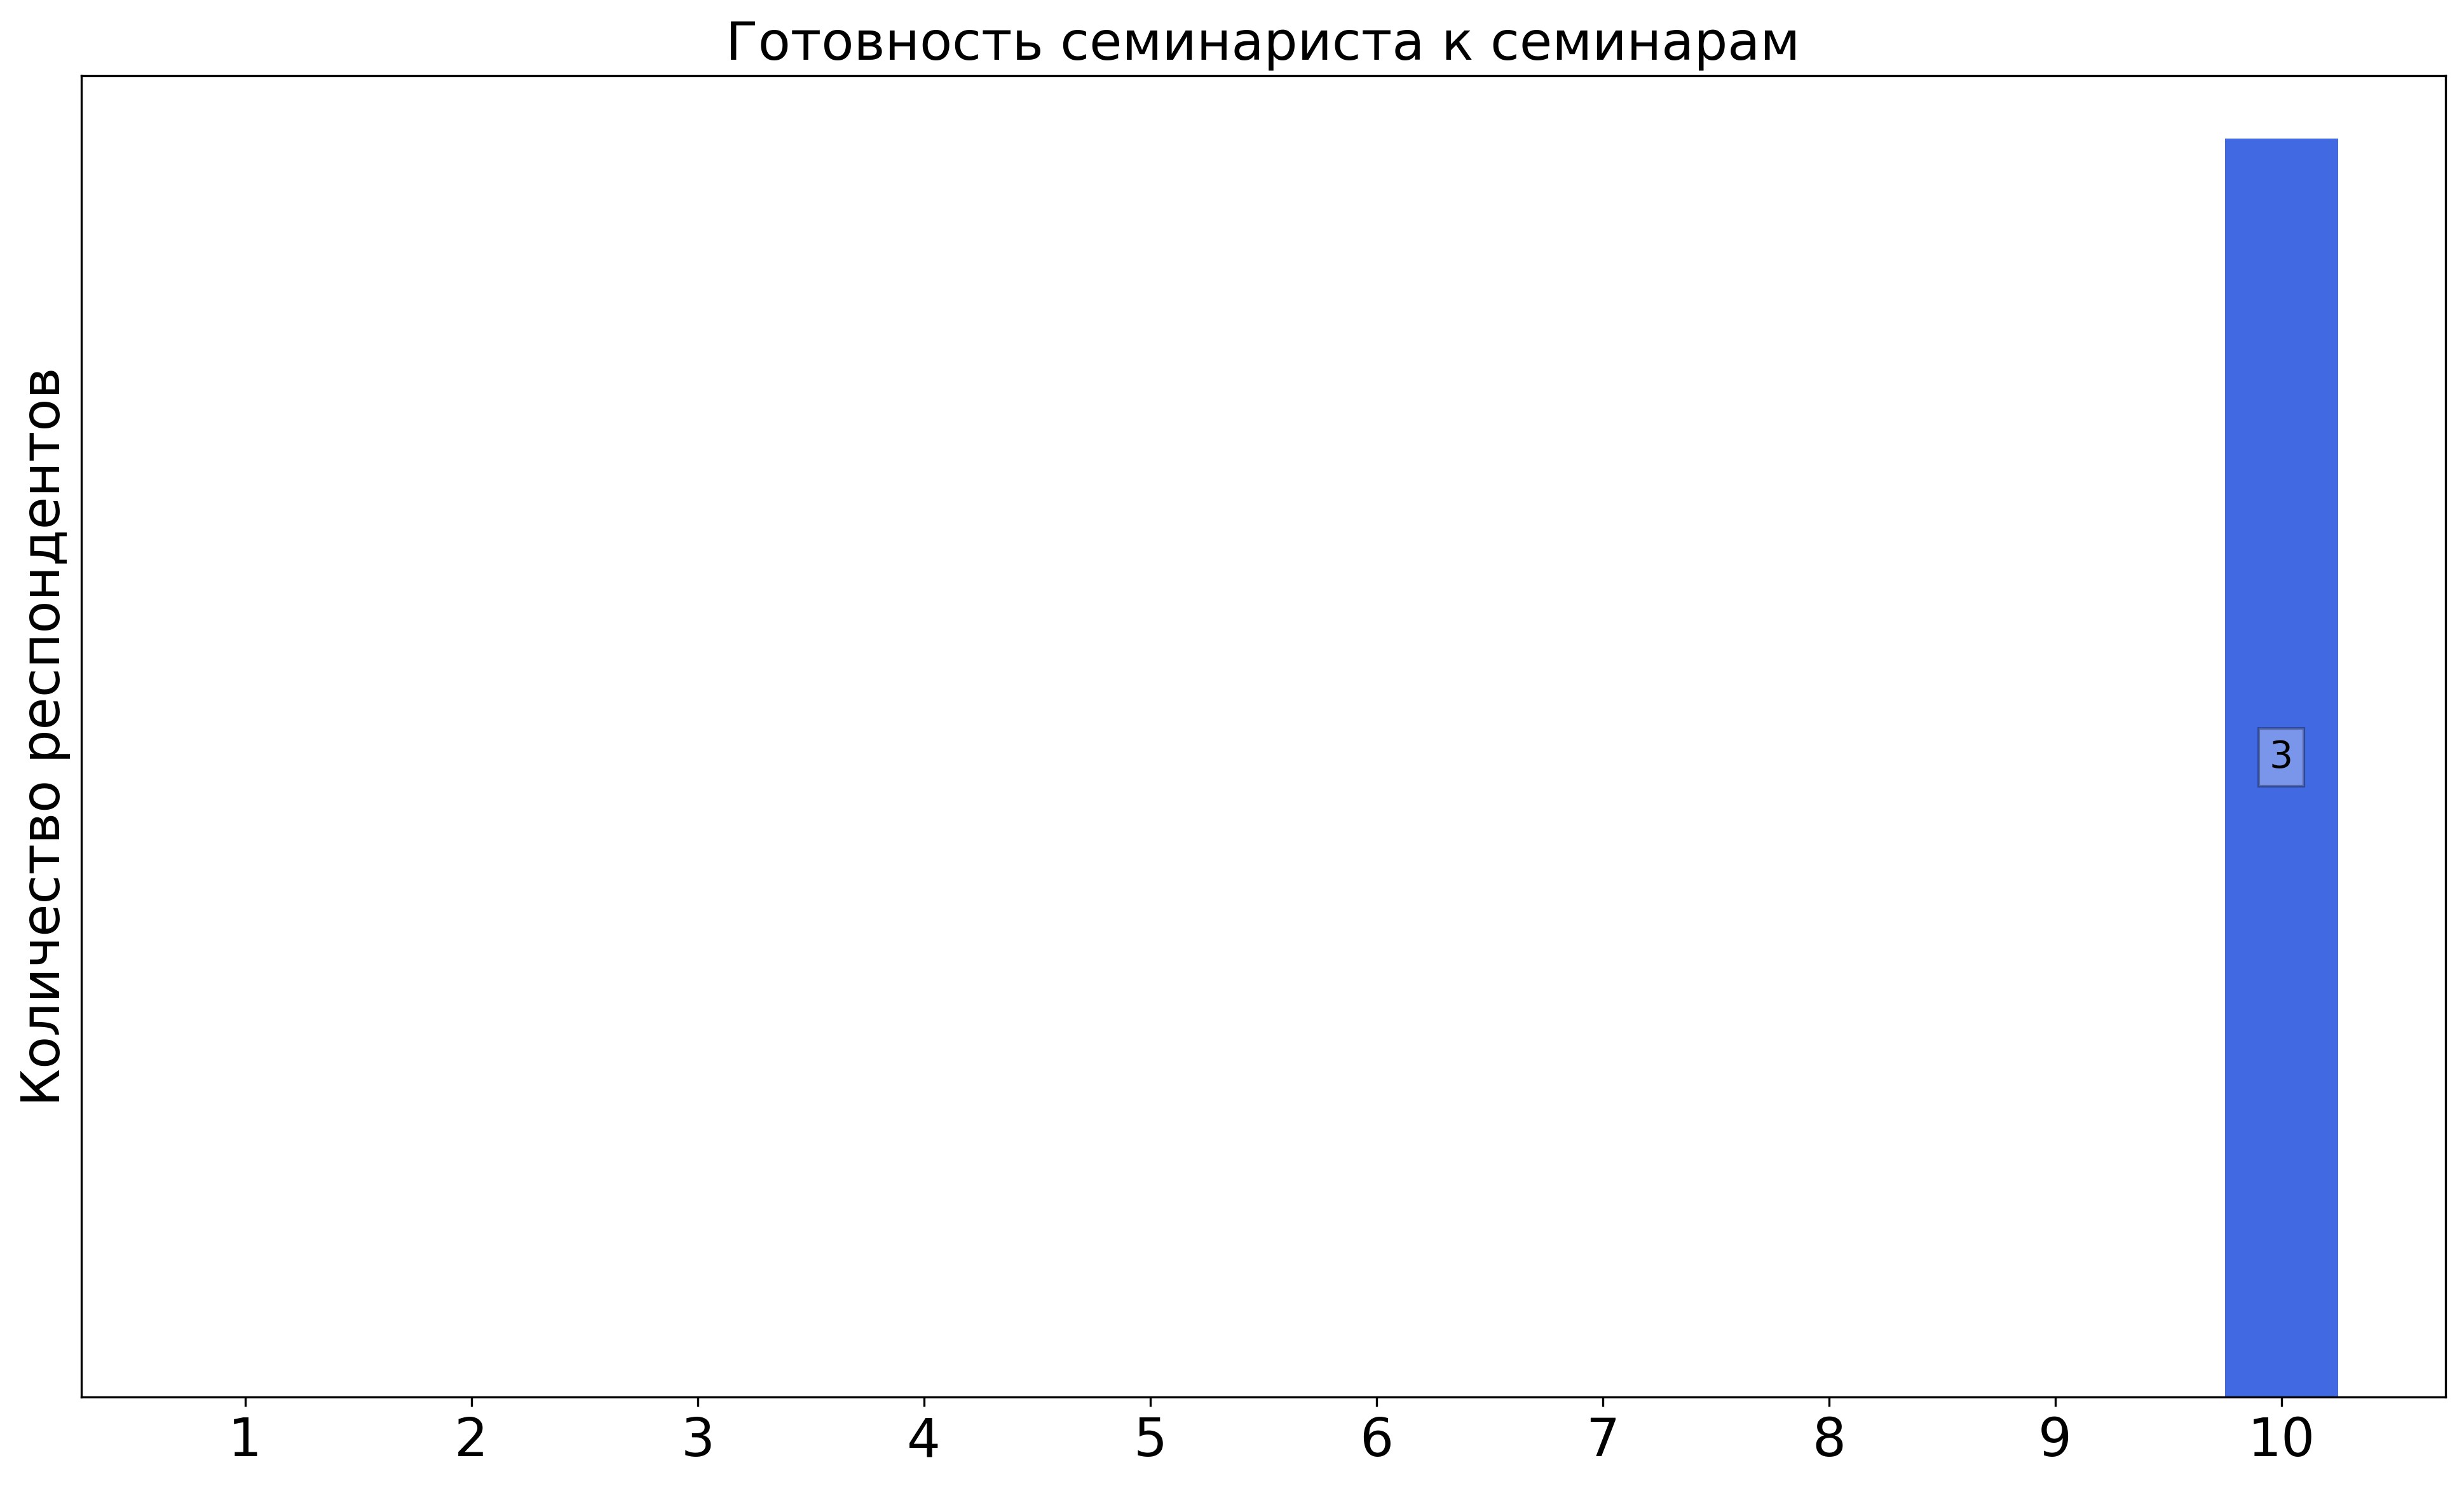
\includegraphics[width=\textwidth]{images/2 course/Дифференциальные уравнения/seminarists-marks-Родин М.М.-1.png}
            \end{subfigure}
            \begin{subfigure}[b]{0.45\textwidth}
                \centering
                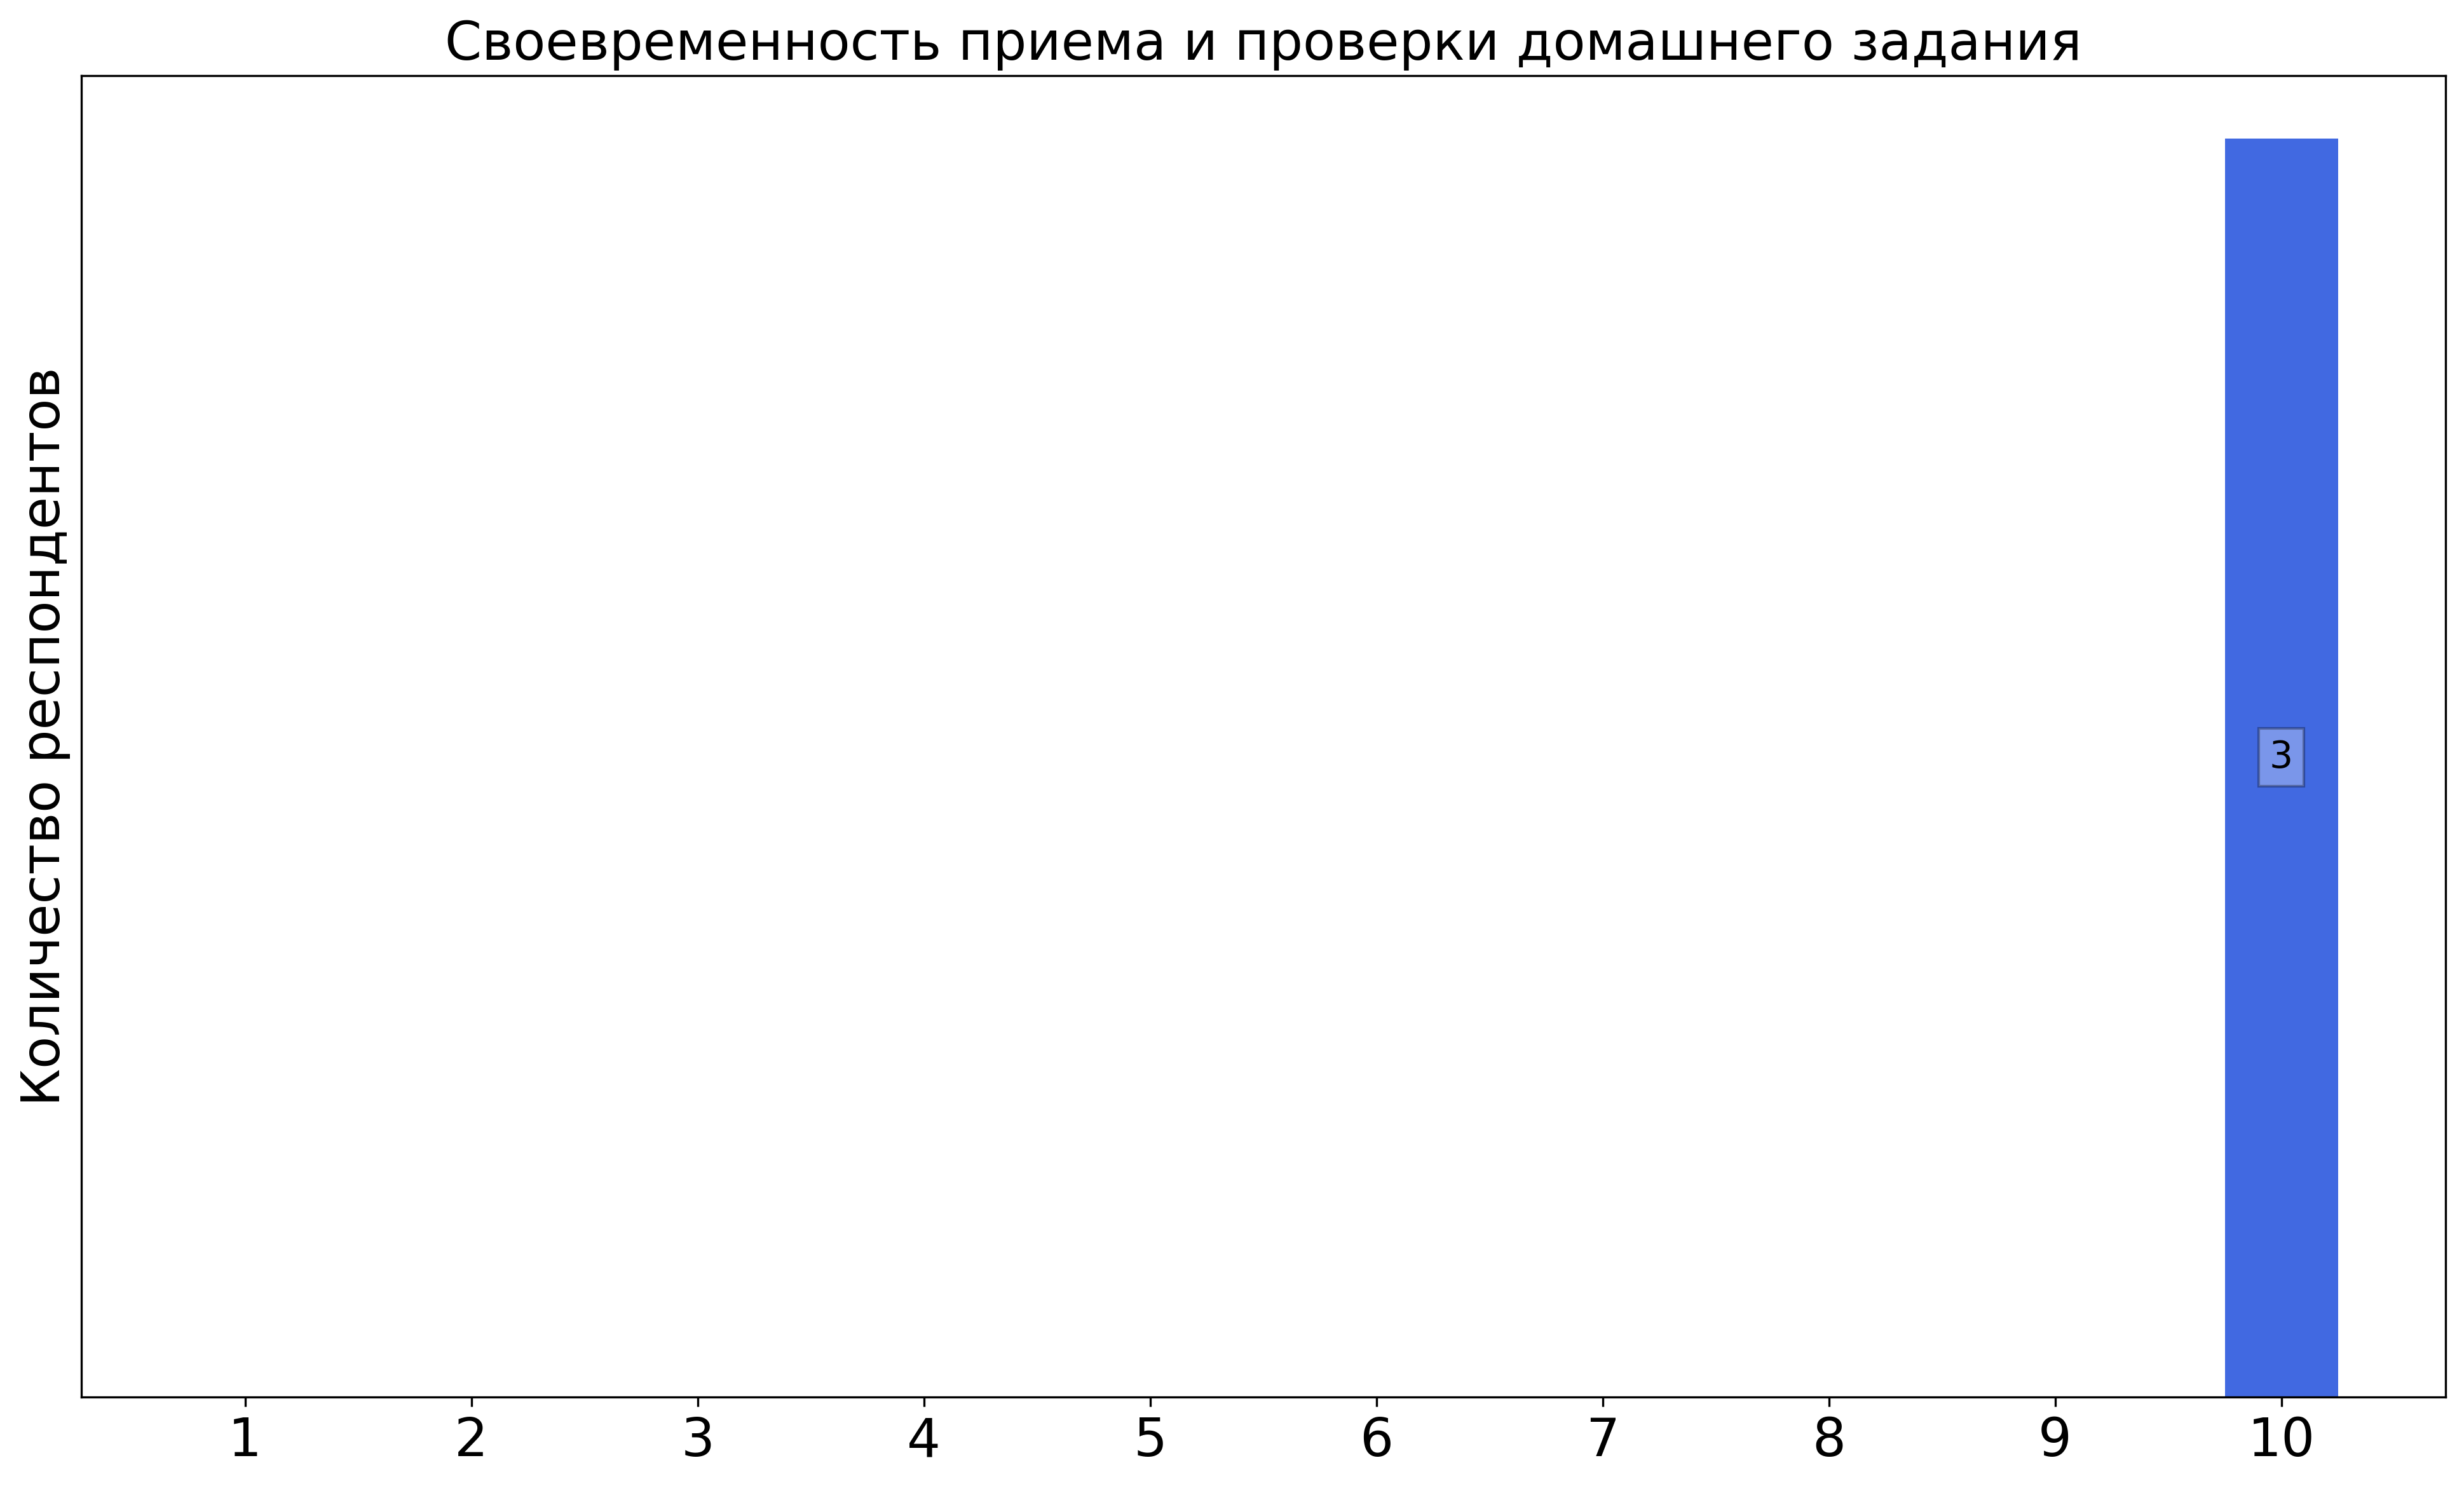
\includegraphics[width=\textwidth]{images/2 course/Дифференциальные уравнения/seminarists-marks-Родин М.М.-2.png}
            \end{subfigure}
            \begin{subfigure}[b]{0.45\textwidth}
                \centering
                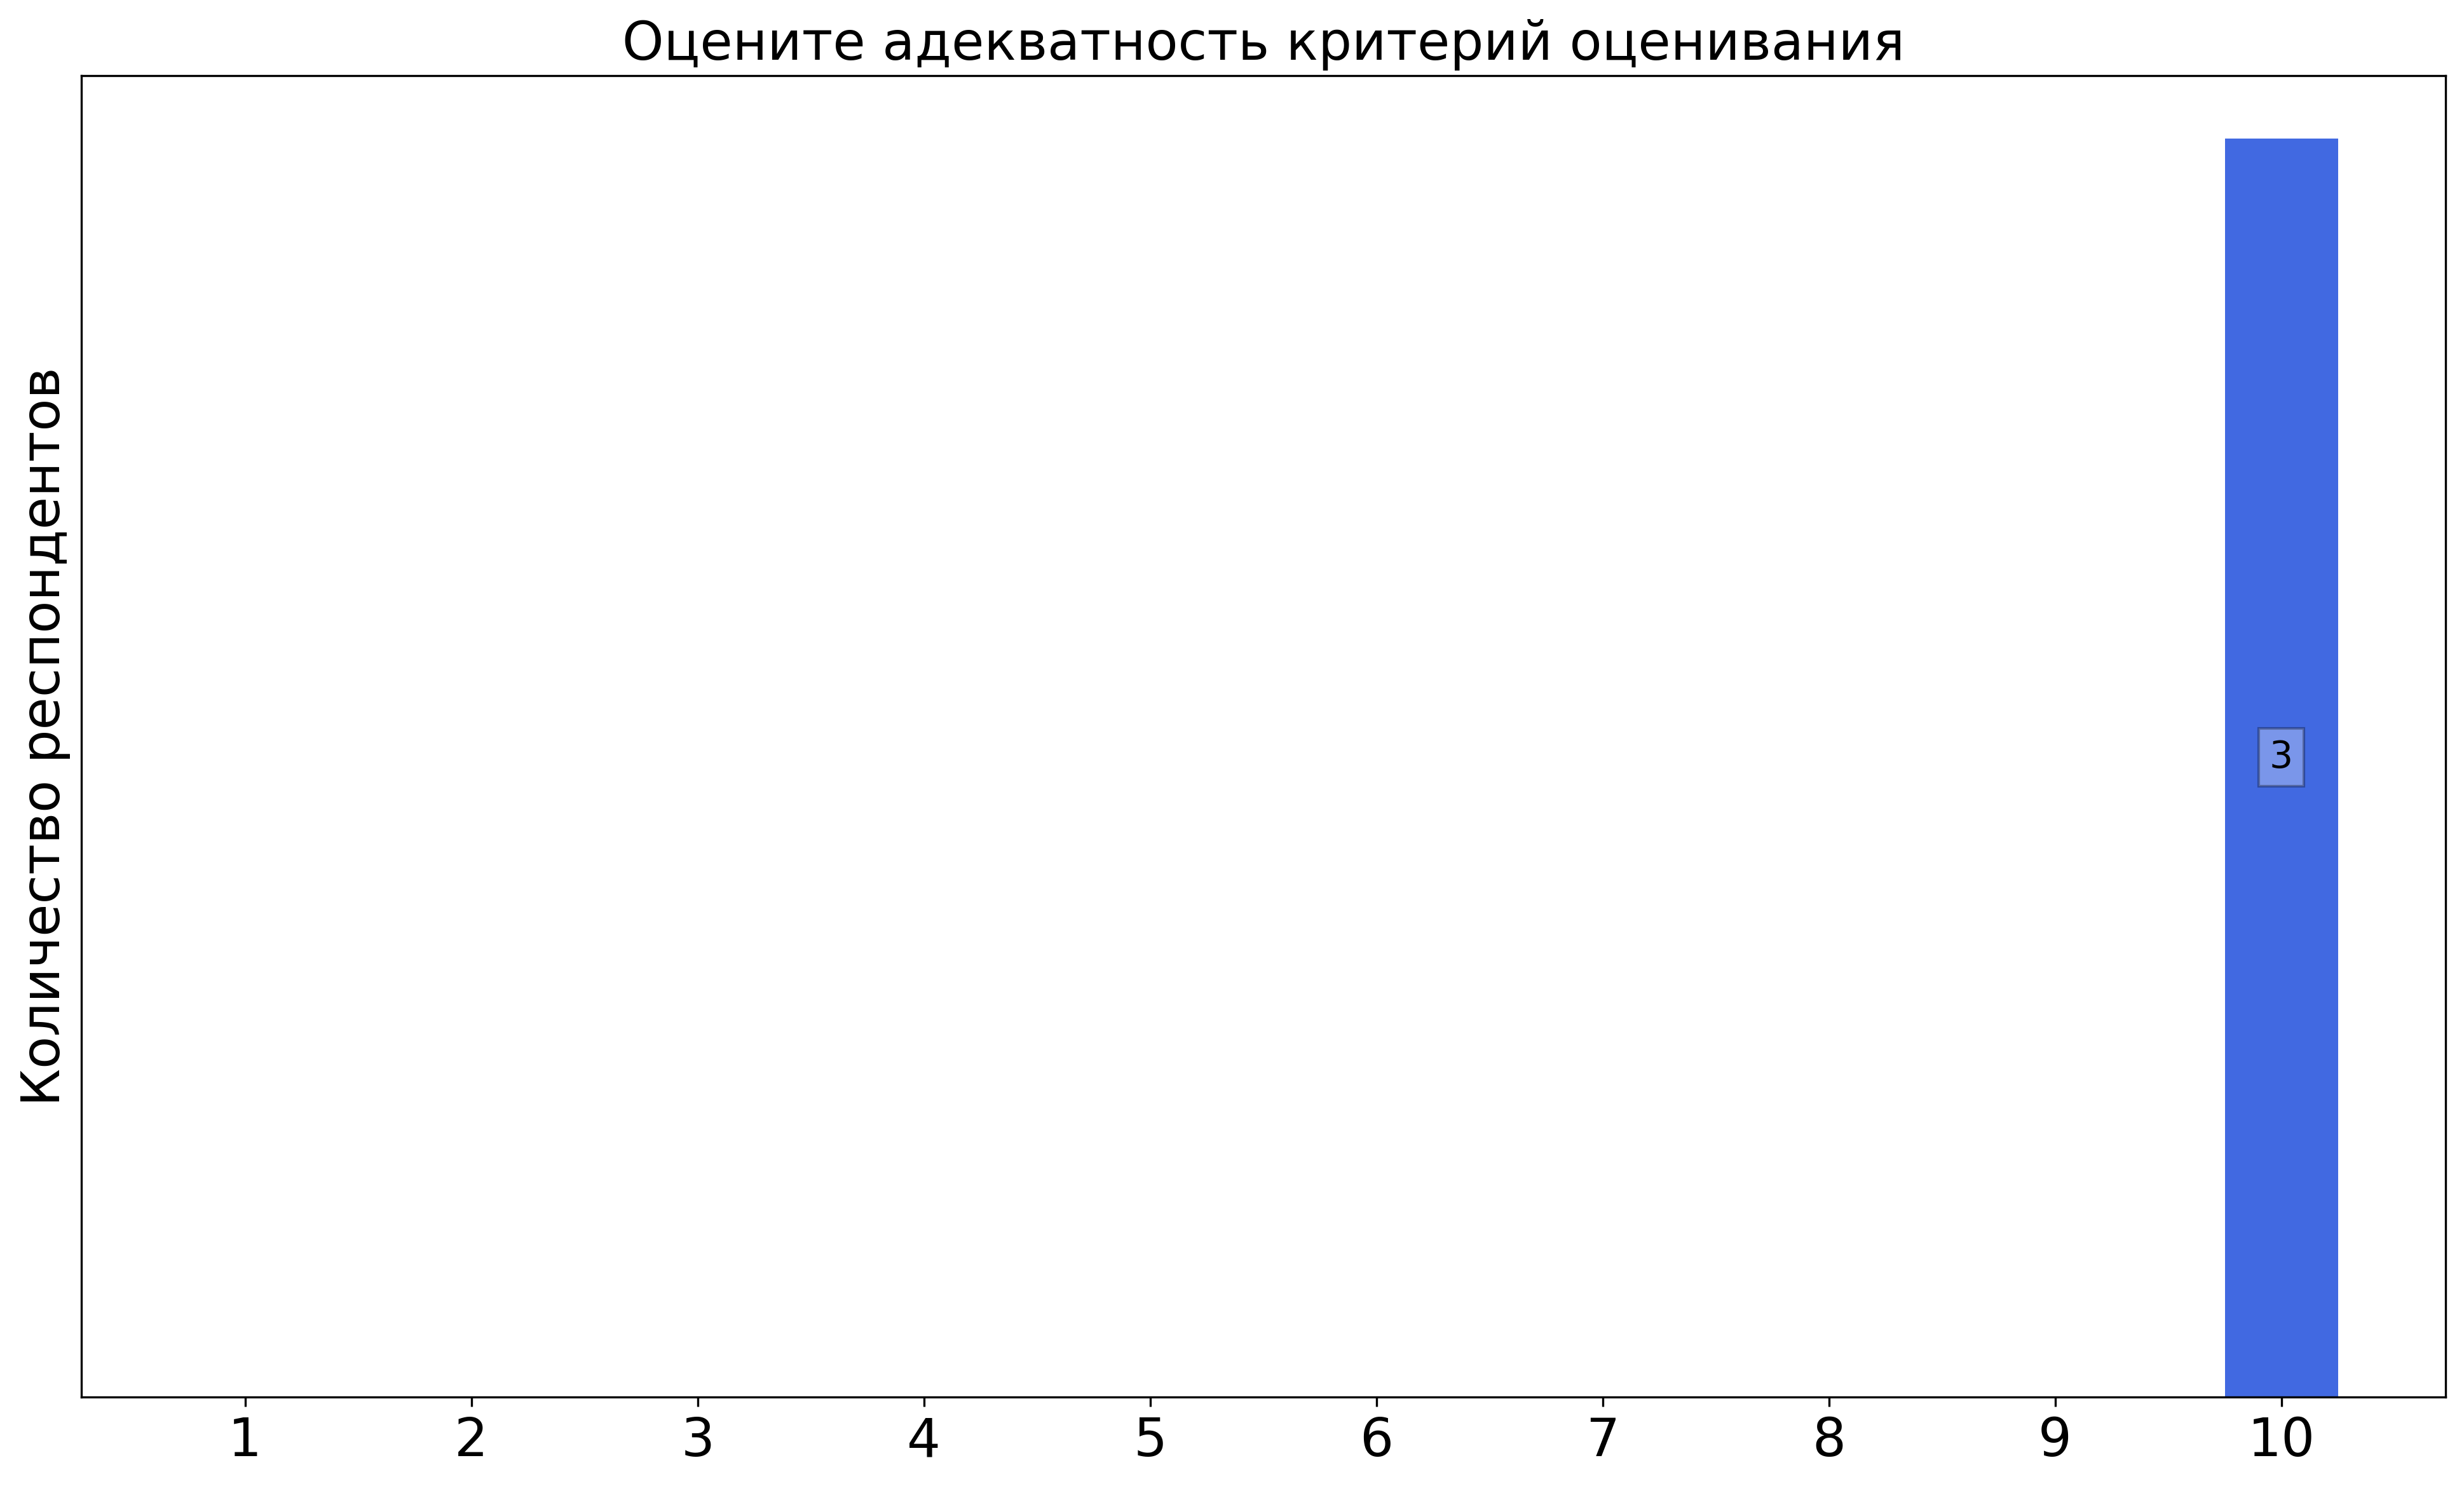
\includegraphics[width=\textwidth]{images/2 course/Дифференциальные уравнения/seminarists-marks-Родин М.М.-3.png}
            \end{subfigure}	
            \caption{Оценки респондентов о качестве преподавания семинаров}
        \end{figure}
        

    \subsubsection{Прочие комментарии и предложения по улучшению курса}
        \begin{commentbox}
            Не делать один экзамен по двум семестрам; всем как будто будет лучше, если разбить материал экзамена на два
        \end{commentbox}